\documentclass[twoside]{book}

% Packages required by doxygen
\usepackage{calc}
\usepackage{doxygen}
\usepackage{graphicx}
\usepackage[utf8]{inputenc}
\usepackage{makeidx}
\usepackage{multicol}
\usepackage{multirow}
\usepackage{textcomp}
\usepackage[table]{xcolor}

% Font selection
\usepackage[T1]{fontenc}
\usepackage{mathptmx}
\usepackage[scaled=.90]{helvet}
\usepackage{courier}
\usepackage{amssymb}
\usepackage{sectsty}
\renewcommand{\familydefault}{\sfdefault}
\allsectionsfont{%
  \fontseries{bc}\selectfont%
  \color{darkgray}%
}
\renewcommand{\DoxyLabelFont}{%
  \fontseries{bc}\selectfont%
  \color{darkgray}%
}

% Page & text layout
\usepackage{geometry}
\geometry{%
  a4paper,%
  top=2.5cm,%
  bottom=2.5cm,%
  left=2.5cm,%
  right=2.5cm%
}
\tolerance=750
\hfuzz=15pt
\hbadness=750
\setlength{\emergencystretch}{15pt}
\setlength{\parindent}{0cm}
\setlength{\parskip}{0.2cm}
\makeatletter
\renewcommand{\paragraph}{%
  \@startsection{paragraph}{4}{0ex}{-1.0ex}{1.0ex}{%
    \normalfont\normalsize\bfseries\SS@parafont%
  }%
}
\renewcommand{\subparagraph}{%
  \@startsection{subparagraph}{5}{0ex}{-1.0ex}{1.0ex}{%
    \normalfont\normalsize\bfseries\SS@subparafont%
  }%
}
\makeatother

% Headers & footers
\usepackage{fancyhdr}
\pagestyle{fancyplain}
\fancyhead[LE]{\fancyplain{}{\bfseries\thepage}}
\fancyhead[CE]{\fancyplain{}{}}
\fancyhead[RE]{\fancyplain{}{\bfseries\leftmark}}
\fancyhead[LO]{\fancyplain{}{\bfseries\rightmark}}
\fancyhead[CO]{\fancyplain{}{}}
\fancyhead[RO]{\fancyplain{}{\bfseries\thepage}}
\fancyfoot[LE]{\fancyplain{}{}}
\fancyfoot[CE]{\fancyplain{}{}}
\fancyfoot[RE]{\fancyplain{}{\bfseries\scriptsize Generated on Tue Jan 6 2015 05\-:27\-:10 for Starcheese\-\_\-\-Trooper by Doxygen }}
\fancyfoot[LO]{\fancyplain{}{\bfseries\scriptsize Generated on Tue Jan 6 2015 05\-:27\-:10 for Starcheese\-\_\-\-Trooper by Doxygen }}
\fancyfoot[CO]{\fancyplain{}{}}
\fancyfoot[RO]{\fancyplain{}{}}
\renewcommand{\footrulewidth}{0.4pt}
\renewcommand{\chaptermark}[1]{%
  \markboth{#1}{}%
}
\renewcommand{\sectionmark}[1]{%
  \markright{\thesection\ #1}%
}

% Indices & bibliography
\usepackage{natbib}
\usepackage[titles]{tocloft}
\setcounter{tocdepth}{3}
\setcounter{secnumdepth}{5}
\makeindex

% Hyperlinks (required, but should be loaded last)
\usepackage{ifpdf}
\ifpdf
  \usepackage[pdftex,pagebackref=true]{hyperref}
\else
  \usepackage[ps2pdf,pagebackref=true]{hyperref}
\fi
\hypersetup{%
  colorlinks=true,%
  linkcolor=blue,%
  citecolor=blue,%
  unicode%
}

% Custom commands
\newcommand{\clearemptydoublepage}{%
  \newpage{\pagestyle{empty}\cleardoublepage}%
}


%===== C O N T E N T S =====

\begin{document}

% Titlepage & ToC
\hypersetup{pageanchor=false}
\pagenumbering{roman}
\begin{titlepage}
\vspace*{7cm}
\begin{center}%
{\Large Starcheese\-\_\-\-Trooper \\[1ex]\large 1.\-0 }\\
\vspace*{1cm}
{\large Generated by Doxygen 1.8.6}\\
\vspace*{0.5cm}
{\small Tue Jan 6 2015 05:27:10}\\
\end{center}
\end{titlepage}
\clearemptydoublepage
\tableofcontents
\clearemptydoublepage
\pagenumbering{arabic}
\hypersetup{pageanchor=true}

%--- Begin generated contents ---
\chapter{Data Structure Index}
\section{Data Structures}
Here are the data structures with brief descriptions\-:\begin{DoxyCompactList}
\item\contentsline{section}{\hyperlink{struct___salle}{\-\_\-\-Salle} }{\pageref{struct___salle}}{}
\item\contentsline{section}{\hyperlink{struct_fantome}{Fantome} \\*Module image }{\pageref{struct_fantome}}{}
\item\contentsline{section}{\hyperlink{struct_fromage}{Fromage} }{\pageref{struct_fromage}}{}
\item\contentsline{section}{\hyperlink{struct_input}{Input} }{\pageref{struct_input}}{}
\item\contentsline{section}{\hyperlink{struct_jeu}{Jeu} }{\pageref{struct_jeu}}{}
\item\contentsline{section}{\hyperlink{struct_projectile}{Projectile} }{\pageref{struct_projectile}}{}
\item\contentsline{section}{\hyperlink{structsdl_jeu}{sdl\-Jeu} }{\pageref{structsdl_jeu}}{}
\item\contentsline{section}{\hyperlink{structs_tableau_dynamique}{s\-Tableau\-Dynamique} }{\pageref{structs_tableau_dynamique}}{}
\item\contentsline{section}{\hyperlink{struct_terrain}{Terrain} }{\pageref{struct_terrain}}{}
\end{DoxyCompactList}

\chapter{File Index}
\section{File List}
Here is a list of all files with brief descriptions\-:\begin{DoxyCompactList}
\item\contentsline{section}{/home/enzo/projet\-\_\-fluide/src/\hyperlink{_fromage_8c}{Fromage.\-c} }{\pageref{_fromage_8c}}{}
\item\contentsline{section}{/home/enzo/projet\-\_\-fluide/src/\hyperlink{_fromage_8h}{Fromage.\-h} }{\pageref{_fromage_8h}}{}
\item\contentsline{section}{/home/enzo/projet\-\_\-fluide/src/\hyperlink{_jeu_8c}{Jeu.\-c} }{\pageref{_jeu_8c}}{}
\item\contentsline{section}{/home/enzo/projet\-\_\-fluide/src/\hyperlink{_jeu_8h}{Jeu.\-h} }{\pageref{_jeu_8h}}{}
\item\contentsline{section}{/home/enzo/projet\-\_\-fluide/src/\hyperlink{main_8c}{main.\-c} }{\pageref{main_8c}}{}
\item\contentsline{section}{/home/enzo/projet\-\_\-fluide/src/\hyperlink{menu_8c}{menu.\-c} }{\pageref{menu_8c}}{}
\item\contentsline{section}{/home/enzo/projet\-\_\-fluide/src/\hyperlink{sdl_jeu_8c}{sdl\-Jeu.\-c} }{\pageref{sdl_jeu_8c}}{}
\item\contentsline{section}{/home/enzo/projet\-\_\-fluide/src/\hyperlink{sdl_jeu_8h}{sdl\-Jeu.\-h} }{\pageref{sdl_jeu_8h}}{}
\item\contentsline{section}{/home/enzo/projet\-\_\-fluide/src/\hyperlink{_terrain_8c}{Terrain.\-c} }{\pageref{_terrain_8c}}{}
\item\contentsline{section}{/home/enzo/projet\-\_\-fluide/src/\hyperlink{_terrain_8h}{Terrain.\-h} }{\pageref{_terrain_8h}}{}
\end{DoxyCompactList}

\chapter{Data Structure Documentation}
\hypertarget{struct___salle}{\section{\-\_\-\-Salle Struct Reference}
\label{struct___salle}\index{\-\_\-\-Salle@{\-\_\-\-Salle}}
}


{\ttfamily \#include $<$Terrain.\-h$>$}



Collaboration diagram for \-\_\-\-Salle\-:\nopagebreak
\begin{figure}[H]
\begin{center}
\leavevmode
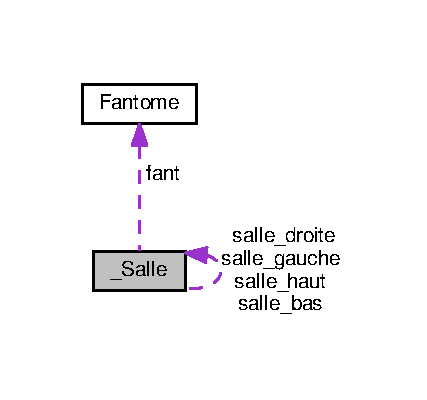
\includegraphics[width=205pt]{struct___salle__coll__graph}
\end{center}
\end{figure}
\subsection*{Data Fields}
\begin{DoxyCompactItemize}
\item 
F\-I\-L\-E $\ast$ \hyperlink{struct___salle_a9b2eab48569631cecdd9c2193f6c0200}{salle\-\_\-actuelle}
\item 
int \hyperlink{struct___salle_a47d84eea0555715068bf00a979b77b27}{nb\-\_\-fantome}
\item 
\hyperlink{struct_fantome}{Fantome} $\ast$ \hyperlink{struct___salle_a569b56072a5a66ebf7db5ab24d371550}{fant}
\item 
struct \hyperlink{struct___salle}{\-\_\-\-Salle} $\ast$ \hyperlink{struct___salle_aa68ee082aa9dcc1ea99c09f46c2b002d}{salle\-\_\-bas}
\item 
struct \hyperlink{struct___salle}{\-\_\-\-Salle} $\ast$ \hyperlink{struct___salle_af393d5336c949f3725154408969f9d32}{salle\-\_\-haut}
\item 
struct \hyperlink{struct___salle}{\-\_\-\-Salle} $\ast$ \hyperlink{struct___salle_abfc5cf6453be9701bad25e9b464e6a63}{salle\-\_\-droite}
\item 
struct \hyperlink{struct___salle}{\-\_\-\-Salle} $\ast$ \hyperlink{struct___salle_af01484c040a5ff15b3f5487acefa31f9}{salle\-\_\-gauche}
\end{DoxyCompactItemize}


\subsection{Detailed Description}


Definition at line 24 of file Terrain.\-h.



\subsection{Field Documentation}
\hypertarget{struct___salle_a569b56072a5a66ebf7db5ab24d371550}{\index{\-\_\-\-Salle@{\-\_\-\-Salle}!fant@{fant}}
\index{fant@{fant}!_Salle@{\-\_\-\-Salle}}
\subsubsection[{fant}]{\setlength{\rightskip}{0pt plus 5cm}{\bf Fantome}$\ast$ fant}}\label{struct___salle_a569b56072a5a66ebf7db5ab24d371550}


Definition at line 30 of file Terrain.\-h.

\hypertarget{struct___salle_a47d84eea0555715068bf00a979b77b27}{\index{\-\_\-\-Salle@{\-\_\-\-Salle}!nb\-\_\-fantome@{nb\-\_\-fantome}}
\index{nb\-\_\-fantome@{nb\-\_\-fantome}!_Salle@{\-\_\-\-Salle}}
\subsubsection[{nb\-\_\-fantome}]{\setlength{\rightskip}{0pt plus 5cm}int nb\-\_\-fantome}}\label{struct___salle_a47d84eea0555715068bf00a979b77b27}


Definition at line 29 of file Terrain.\-h.

\hypertarget{struct___salle_a9b2eab48569631cecdd9c2193f6c0200}{\index{\-\_\-\-Salle@{\-\_\-\-Salle}!salle\-\_\-actuelle@{salle\-\_\-actuelle}}
\index{salle\-\_\-actuelle@{salle\-\_\-actuelle}!_Salle@{\-\_\-\-Salle}}
\subsubsection[{salle\-\_\-actuelle}]{\setlength{\rightskip}{0pt plus 5cm}F\-I\-L\-E$\ast$ salle\-\_\-actuelle}}\label{struct___salle_a9b2eab48569631cecdd9c2193f6c0200}


Definition at line 28 of file Terrain.\-h.

\hypertarget{struct___salle_aa68ee082aa9dcc1ea99c09f46c2b002d}{\index{\-\_\-\-Salle@{\-\_\-\-Salle}!salle\-\_\-bas@{salle\-\_\-bas}}
\index{salle\-\_\-bas@{salle\-\_\-bas}!_Salle@{\-\_\-\-Salle}}
\subsubsection[{salle\-\_\-bas}]{\setlength{\rightskip}{0pt plus 5cm}struct {\bf \-\_\-\-Salle}$\ast$ salle\-\_\-bas}}\label{struct___salle_aa68ee082aa9dcc1ea99c09f46c2b002d}


Definition at line 31 of file Terrain.\-h.

\hypertarget{struct___salle_abfc5cf6453be9701bad25e9b464e6a63}{\index{\-\_\-\-Salle@{\-\_\-\-Salle}!salle\-\_\-droite@{salle\-\_\-droite}}
\index{salle\-\_\-droite@{salle\-\_\-droite}!_Salle@{\-\_\-\-Salle}}
\subsubsection[{salle\-\_\-droite}]{\setlength{\rightskip}{0pt plus 5cm}struct {\bf \-\_\-\-Salle}$\ast$ salle\-\_\-droite}}\label{struct___salle_abfc5cf6453be9701bad25e9b464e6a63}


Definition at line 33 of file Terrain.\-h.

\hypertarget{struct___salle_af01484c040a5ff15b3f5487acefa31f9}{\index{\-\_\-\-Salle@{\-\_\-\-Salle}!salle\-\_\-gauche@{salle\-\_\-gauche}}
\index{salle\-\_\-gauche@{salle\-\_\-gauche}!_Salle@{\-\_\-\-Salle}}
\subsubsection[{salle\-\_\-gauche}]{\setlength{\rightskip}{0pt plus 5cm}struct {\bf \-\_\-\-Salle}$\ast$ salle\-\_\-gauche}}\label{struct___salle_af01484c040a5ff15b3f5487acefa31f9}


Definition at line 34 of file Terrain.\-h.

\hypertarget{struct___salle_af393d5336c949f3725154408969f9d32}{\index{\-\_\-\-Salle@{\-\_\-\-Salle}!salle\-\_\-haut@{salle\-\_\-haut}}
\index{salle\-\_\-haut@{salle\-\_\-haut}!_Salle@{\-\_\-\-Salle}}
\subsubsection[{salle\-\_\-haut}]{\setlength{\rightskip}{0pt plus 5cm}struct {\bf \-\_\-\-Salle}$\ast$ salle\-\_\-haut}}\label{struct___salle_af393d5336c949f3725154408969f9d32}


Definition at line 32 of file Terrain.\-h.



The documentation for this struct was generated from the following file\-:\begin{DoxyCompactItemize}
\item 
/home/enzo/projet\-\_\-fluide/src/\hyperlink{_terrain_8h}{Terrain.\-h}\end{DoxyCompactItemize}

\hypertarget{struct_fantome}{\section{Fantome Struct Reference}
\label{struct_fantome}\index{Fantome@{Fantome}}
}


Module image.  




{\ttfamily \#include $<$Terrain.\-h$>$}

\subsection*{Public Types}
\begin{DoxyCompactItemize}
\item 
enum \{ \hyperlink{struct_fantome_a06fc87d81c62e9abb8790b6e5713c55ba79f680205087956546ae263797bd1343}{D\-R\-O\-I\-T\-E}, 
\hyperlink{struct_fantome_a06fc87d81c62e9abb8790b6e5713c55ba4ee960d97b04a1f22ed7ff81c7aa2e86}{G\-A\-U\-C\-H\-E}, 
\hyperlink{struct_fantome_a06fc87d81c62e9abb8790b6e5713c55ba5c97701a87d36c8f2c0de80c5865b8e2}{H\-A\-U\-T}, 
\hyperlink{struct_fantome_a06fc87d81c62e9abb8790b6e5713c55ba4b07baad9e862178efeac3e522475caa}{B\-A\-S}
 \}
\end{DoxyCompactItemize}
\subsection*{Data Fields}
\begin{DoxyCompactItemize}
\item 
int \hyperlink{struct_fantome_a6150e0515f7202e2fb518f7206ed97dc}{x}
\item 
int \hyperlink{struct_fantome_a0a2f84ed7838f07779ae24c5a9086d33}{y}
\item 
int \hyperlink{struct_fantome_a80e06e27760b1b0623a2aac7dc1bc191}{mort}
\item 
int \hyperlink{struct_fantome_ae8ffd4287a5e2d2b9c8a268be76a8b89}{proche}
\item 
enum Fantome\-:: \{ ... \}  \hyperlink{struct_fantome_a3b781c6f2ff99911d58614aedbf40c2a}{direction}
\end{DoxyCompactItemize}


\subsection{Detailed Description}
Module image. 

\begin{DoxyAuthor}{Author}
Ambrosino Gwenaël Lebrun Enzo 
\end{DoxyAuthor}
\begin{DoxyVersion}{Version}
1.\-0 
\end{DoxyVersion}
\begin{DoxyDate}{Date}
2014/01/06 
\end{DoxyDate}


Definition at line 15 of file Terrain.\-h.



\subsection{Member Enumeration Documentation}
\hypertarget{struct_fantome_a06fc87d81c62e9abb8790b6e5713c55b}{\subsubsection[{anonymous enum}]{\setlength{\rightskip}{0pt plus 5cm}anonymous enum}}\label{struct_fantome_a06fc87d81c62e9abb8790b6e5713c55b}
\begin{Desc}
\item[Enumerator]\par
\begin{description}
\index{D\-R\-O\-I\-T\-E@{D\-R\-O\-I\-T\-E}!Fantome@{Fantome}}\index{Fantome@{Fantome}!D\-R\-O\-I\-T\-E@{D\-R\-O\-I\-T\-E}}\item[{\em 
\hypertarget{struct_fantome_a06fc87d81c62e9abb8790b6e5713c55ba79f680205087956546ae263797bd1343}{D\-R\-O\-I\-T\-E}\label{struct_fantome_a06fc87d81c62e9abb8790b6e5713c55ba79f680205087956546ae263797bd1343}
}]\index{G\-A\-U\-C\-H\-E@{G\-A\-U\-C\-H\-E}!Fantome@{Fantome}}\index{Fantome@{Fantome}!G\-A\-U\-C\-H\-E@{G\-A\-U\-C\-H\-E}}\item[{\em 
\hypertarget{struct_fantome_a06fc87d81c62e9abb8790b6e5713c55ba4ee960d97b04a1f22ed7ff81c7aa2e86}{G\-A\-U\-C\-H\-E}\label{struct_fantome_a06fc87d81c62e9abb8790b6e5713c55ba4ee960d97b04a1f22ed7ff81c7aa2e86}
}]\index{H\-A\-U\-T@{H\-A\-U\-T}!Fantome@{Fantome}}\index{Fantome@{Fantome}!H\-A\-U\-T@{H\-A\-U\-T}}\item[{\em 
\hypertarget{struct_fantome_a06fc87d81c62e9abb8790b6e5713c55ba5c97701a87d36c8f2c0de80c5865b8e2}{H\-A\-U\-T}\label{struct_fantome_a06fc87d81c62e9abb8790b6e5713c55ba5c97701a87d36c8f2c0de80c5865b8e2}
}]\index{B\-A\-S@{B\-A\-S}!Fantome@{Fantome}}\index{Fantome@{Fantome}!B\-A\-S@{B\-A\-S}}\item[{\em 
\hypertarget{struct_fantome_a06fc87d81c62e9abb8790b6e5713c55ba4b07baad9e862178efeac3e522475caa}{B\-A\-S}\label{struct_fantome_a06fc87d81c62e9abb8790b6e5713c55ba4b07baad9e862178efeac3e522475caa}
}]\end{description}
\end{Desc}


Definition at line 20 of file Terrain.\-h.



\subsection{Field Documentation}
\hypertarget{struct_fantome_a3b781c6f2ff99911d58614aedbf40c2a}{\index{Fantome@{Fantome}!direction@{direction}}
\index{direction@{direction}!Fantome@{Fantome}}
\subsubsection[{direction}]{\setlength{\rightskip}{0pt plus 5cm}enum \{ ... \}   direction}}\label{struct_fantome_a3b781c6f2ff99911d58614aedbf40c2a}
\hypertarget{struct_fantome_a80e06e27760b1b0623a2aac7dc1bc191}{\index{Fantome@{Fantome}!mort@{mort}}
\index{mort@{mort}!Fantome@{Fantome}}
\subsubsection[{mort}]{\setlength{\rightskip}{0pt plus 5cm}int mort}}\label{struct_fantome_a80e06e27760b1b0623a2aac7dc1bc191}


Definition at line 18 of file Terrain.\-h.

\hypertarget{struct_fantome_ae8ffd4287a5e2d2b9c8a268be76a8b89}{\index{Fantome@{Fantome}!proche@{proche}}
\index{proche@{proche}!Fantome@{Fantome}}
\subsubsection[{proche}]{\setlength{\rightskip}{0pt plus 5cm}int proche}}\label{struct_fantome_ae8ffd4287a5e2d2b9c8a268be76a8b89}


Definition at line 19 of file Terrain.\-h.

\hypertarget{struct_fantome_a6150e0515f7202e2fb518f7206ed97dc}{\index{Fantome@{Fantome}!x@{x}}
\index{x@{x}!Fantome@{Fantome}}
\subsubsection[{x}]{\setlength{\rightskip}{0pt plus 5cm}int x}}\label{struct_fantome_a6150e0515f7202e2fb518f7206ed97dc}


Definition at line 17 of file Terrain.\-h.

\hypertarget{struct_fantome_a0a2f84ed7838f07779ae24c5a9086d33}{\index{Fantome@{Fantome}!y@{y}}
\index{y@{y}!Fantome@{Fantome}}
\subsubsection[{y}]{\setlength{\rightskip}{0pt plus 5cm}int y}}\label{struct_fantome_a0a2f84ed7838f07779ae24c5a9086d33}


Definition at line 17 of file Terrain.\-h.



The documentation for this struct was generated from the following file\-:\begin{DoxyCompactItemize}
\item 
/home/enzo/projet\-\_\-fluide/src/\hyperlink{_terrain_8h}{Terrain.\-h}\end{DoxyCompactItemize}

\hypertarget{struct_fromage}{\section{Fromage Struct Reference}
\label{struct_fromage}\index{Fromage@{Fromage}}
}


{\ttfamily \#include $<$Fromage.\-h$>$}

\subsection*{Data Fields}
\begin{DoxyCompactItemize}
\item 
S\-D\-L\-\_\-\-Rect \hyperlink{struct_fromage_a4b36eb370ba51290847183a8da37db31}{source}
\item 
S\-D\-L\-\_\-\-Rect \hyperlink{struct_fromage_a1d4c1bb15892e31b9af1f4fcf5d31fab}{dest}
\item 
S\-D\-L\-\_\-\-Rect \hyperlink{struct_fromage_a0fcd2fb6981b924459a467441bf99419}{posfrom}
\item 
int \hyperlink{struct_fromage_a74f0f2591e5f65bf792b2c3c67817d78}{largeur}
\item 
int \hyperlink{struct_fromage_a5e94a2f98c16e8b6860f95c99da1c0d3}{hauteur}
\item 
float \hyperlink{struct_fromage_ad0da36b2558901e21e7a30f6c227a45e}{x}
\item 
float \hyperlink{struct_fromage_aa4f0d3eebc3c443f9be81bf48561a217}{y}
\item 
float \hyperlink{struct_fromage_a4a1cf9110d6aeb65343be53dbfb5f5e9}{c\-\_\-x}
\item 
float \hyperlink{struct_fromage_a948ae6c4d8e4618590ebc2c1b13d0451}{c\-\_\-y}
\item 
float \hyperlink{struct_fromage_acc9793492dfac2fbf5259cf46e4d6067}{c\-\_\-max\-\_\-x}
\item 
float \hyperlink{struct_fromage_a6fc56c58b8aa8a676f9d3c473b35dbe0}{c\-\_\-max\-\_\-y}
\item 
float \hyperlink{struct_fromage_ab3ac8e1dc34f396339f93c01d2782044}{acc\-\_\-x}
\item 
float \hyperlink{struct_fromage_a781272f25ca67525c9902c98577122e3}{acc\-\_\-y}
\item 
int \hyperlink{struct_fromage_a886d551d5381dc3e53f17825ffc51641}{direction}
\item 
int \hyperlink{struct_fromage_a528d22a2a1651a4831eb643884a3c718}{orientation}
\item 
int \hyperlink{struct_fromage_a9aa790f93d2d067a4f5608fdb8409f94}{hp}
\item 
float \hyperlink{struct_fromage_aef55e1775d611bfea0196692da1a0bc5}{vitesse}
\item 
int \hyperlink{struct_fromage_a63c99fe1f6b99dd1d4a139352023459a}{anim}
\item 
int \hyperlink{struct_fromage_a7a1d95344655c2e0df3ebbc6a282ae1f}{anim\-\_\-courante}
\item 
int \hyperlink{struct_fromage_a9f94aff026d82b8ba1067a997eb23102}{temps\-\_\-anim}
\item 
int \hyperlink{struct_fromage_af6c2caeb693a1e84b84beecae50891b4}{temps\-\_\-anim\-\_\-courante}
\item 
int \hyperlink{struct_fromage_a261ecb9a33ea9b7faaefeb6a4be47f5b}{total\-\_\-anims}
\end{DoxyCompactItemize}


\subsection{Detailed Description}


Definition at line 6 of file Fromage.\-h.



\subsection{Field Documentation}
\hypertarget{struct_fromage_ab3ac8e1dc34f396339f93c01d2782044}{\index{Fromage@{Fromage}!acc\-\_\-x@{acc\-\_\-x}}
\index{acc\-\_\-x@{acc\-\_\-x}!Fromage@{Fromage}}
\subsubsection[{acc\-\_\-x}]{\setlength{\rightskip}{0pt plus 5cm}float acc\-\_\-x}}\label{struct_fromage_ab3ac8e1dc34f396339f93c01d2782044}


Definition at line 15 of file Fromage.\-h.

\hypertarget{struct_fromage_a781272f25ca67525c9902c98577122e3}{\index{Fromage@{Fromage}!acc\-\_\-y@{acc\-\_\-y}}
\index{acc\-\_\-y@{acc\-\_\-y}!Fromage@{Fromage}}
\subsubsection[{acc\-\_\-y}]{\setlength{\rightskip}{0pt plus 5cm}float acc\-\_\-y}}\label{struct_fromage_a781272f25ca67525c9902c98577122e3}


Definition at line 15 of file Fromage.\-h.

\hypertarget{struct_fromage_a63c99fe1f6b99dd1d4a139352023459a}{\index{Fromage@{Fromage}!anim@{anim}}
\index{anim@{anim}!Fromage@{Fromage}}
\subsubsection[{anim}]{\setlength{\rightskip}{0pt plus 5cm}int anim}}\label{struct_fromage_a63c99fe1f6b99dd1d4a139352023459a}


Definition at line 20 of file Fromage.\-h.

\hypertarget{struct_fromage_a7a1d95344655c2e0df3ebbc6a282ae1f}{\index{Fromage@{Fromage}!anim\-\_\-courante@{anim\-\_\-courante}}
\index{anim\-\_\-courante@{anim\-\_\-courante}!Fromage@{Fromage}}
\subsubsection[{anim\-\_\-courante}]{\setlength{\rightskip}{0pt plus 5cm}int anim\-\_\-courante}}\label{struct_fromage_a7a1d95344655c2e0df3ebbc6a282ae1f}


Definition at line 21 of file Fromage.\-h.

\hypertarget{struct_fromage_acc9793492dfac2fbf5259cf46e4d6067}{\index{Fromage@{Fromage}!c\-\_\-max\-\_\-x@{c\-\_\-max\-\_\-x}}
\index{c\-\_\-max\-\_\-x@{c\-\_\-max\-\_\-x}!Fromage@{Fromage}}
\subsubsection[{c\-\_\-max\-\_\-x}]{\setlength{\rightskip}{0pt plus 5cm}float c\-\_\-max\-\_\-x}}\label{struct_fromage_acc9793492dfac2fbf5259cf46e4d6067}


Definition at line 14 of file Fromage.\-h.

\hypertarget{struct_fromage_a6fc56c58b8aa8a676f9d3c473b35dbe0}{\index{Fromage@{Fromage}!c\-\_\-max\-\_\-y@{c\-\_\-max\-\_\-y}}
\index{c\-\_\-max\-\_\-y@{c\-\_\-max\-\_\-y}!Fromage@{Fromage}}
\subsubsection[{c\-\_\-max\-\_\-y}]{\setlength{\rightskip}{0pt plus 5cm}float c\-\_\-max\-\_\-y}}\label{struct_fromage_a6fc56c58b8aa8a676f9d3c473b35dbe0}


Definition at line 14 of file Fromage.\-h.

\hypertarget{struct_fromage_a4a1cf9110d6aeb65343be53dbfb5f5e9}{\index{Fromage@{Fromage}!c\-\_\-x@{c\-\_\-x}}
\index{c\-\_\-x@{c\-\_\-x}!Fromage@{Fromage}}
\subsubsection[{c\-\_\-x}]{\setlength{\rightskip}{0pt plus 5cm}float c\-\_\-x}}\label{struct_fromage_a4a1cf9110d6aeb65343be53dbfb5f5e9}


Definition at line 14 of file Fromage.\-h.

\hypertarget{struct_fromage_a948ae6c4d8e4618590ebc2c1b13d0451}{\index{Fromage@{Fromage}!c\-\_\-y@{c\-\_\-y}}
\index{c\-\_\-y@{c\-\_\-y}!Fromage@{Fromage}}
\subsubsection[{c\-\_\-y}]{\setlength{\rightskip}{0pt plus 5cm}float c\-\_\-y}}\label{struct_fromage_a948ae6c4d8e4618590ebc2c1b13d0451}


Definition at line 14 of file Fromage.\-h.

\hypertarget{struct_fromage_a1d4c1bb15892e31b9af1f4fcf5d31fab}{\index{Fromage@{Fromage}!dest@{dest}}
\index{dest@{dest}!Fromage@{Fromage}}
\subsubsection[{dest}]{\setlength{\rightskip}{0pt plus 5cm}S\-D\-L\-\_\-\-Rect dest}}\label{struct_fromage_a1d4c1bb15892e31b9af1f4fcf5d31fab}


Definition at line 9 of file Fromage.\-h.

\hypertarget{struct_fromage_a886d551d5381dc3e53f17825ffc51641}{\index{Fromage@{Fromage}!direction@{direction}}
\index{direction@{direction}!Fromage@{Fromage}}
\subsubsection[{direction}]{\setlength{\rightskip}{0pt plus 5cm}int direction}}\label{struct_fromage_a886d551d5381dc3e53f17825ffc51641}


Definition at line 16 of file Fromage.\-h.

\hypertarget{struct_fromage_a5e94a2f98c16e8b6860f95c99da1c0d3}{\index{Fromage@{Fromage}!hauteur@{hauteur}}
\index{hauteur@{hauteur}!Fromage@{Fromage}}
\subsubsection[{hauteur}]{\setlength{\rightskip}{0pt plus 5cm}int hauteur}}\label{struct_fromage_a5e94a2f98c16e8b6860f95c99da1c0d3}


Definition at line 11 of file Fromage.\-h.

\hypertarget{struct_fromage_a9aa790f93d2d067a4f5608fdb8409f94}{\index{Fromage@{Fromage}!hp@{hp}}
\index{hp@{hp}!Fromage@{Fromage}}
\subsubsection[{hp}]{\setlength{\rightskip}{0pt plus 5cm}int hp}}\label{struct_fromage_a9aa790f93d2d067a4f5608fdb8409f94}


Definition at line 18 of file Fromage.\-h.

\hypertarget{struct_fromage_a74f0f2591e5f65bf792b2c3c67817d78}{\index{Fromage@{Fromage}!largeur@{largeur}}
\index{largeur@{largeur}!Fromage@{Fromage}}
\subsubsection[{largeur}]{\setlength{\rightskip}{0pt plus 5cm}int largeur}}\label{struct_fromage_a74f0f2591e5f65bf792b2c3c67817d78}


Definition at line 11 of file Fromage.\-h.

\hypertarget{struct_fromage_a528d22a2a1651a4831eb643884a3c718}{\index{Fromage@{Fromage}!orientation@{orientation}}
\index{orientation@{orientation}!Fromage@{Fromage}}
\subsubsection[{orientation}]{\setlength{\rightskip}{0pt plus 5cm}int orientation}}\label{struct_fromage_a528d22a2a1651a4831eb643884a3c718}


Definition at line 17 of file Fromage.\-h.

\hypertarget{struct_fromage_a0fcd2fb6981b924459a467441bf99419}{\index{Fromage@{Fromage}!posfrom@{posfrom}}
\index{posfrom@{posfrom}!Fromage@{Fromage}}
\subsubsection[{posfrom}]{\setlength{\rightskip}{0pt plus 5cm}S\-D\-L\-\_\-\-Rect posfrom}}\label{struct_fromage_a0fcd2fb6981b924459a467441bf99419}


Definition at line 10 of file Fromage.\-h.

\hypertarget{struct_fromage_a4b36eb370ba51290847183a8da37db31}{\index{Fromage@{Fromage}!source@{source}}
\index{source@{source}!Fromage@{Fromage}}
\subsubsection[{source}]{\setlength{\rightskip}{0pt plus 5cm}S\-D\-L\-\_\-\-Rect source}}\label{struct_fromage_a4b36eb370ba51290847183a8da37db31}


Definition at line 8 of file Fromage.\-h.

\hypertarget{struct_fromage_a9f94aff026d82b8ba1067a997eb23102}{\index{Fromage@{Fromage}!temps\-\_\-anim@{temps\-\_\-anim}}
\index{temps\-\_\-anim@{temps\-\_\-anim}!Fromage@{Fromage}}
\subsubsection[{temps\-\_\-anim}]{\setlength{\rightskip}{0pt plus 5cm}int temps\-\_\-anim}}\label{struct_fromage_a9f94aff026d82b8ba1067a997eb23102}


Definition at line 22 of file Fromage.\-h.

\hypertarget{struct_fromage_af6c2caeb693a1e84b84beecae50891b4}{\index{Fromage@{Fromage}!temps\-\_\-anim\-\_\-courante@{temps\-\_\-anim\-\_\-courante}}
\index{temps\-\_\-anim\-\_\-courante@{temps\-\_\-anim\-\_\-courante}!Fromage@{Fromage}}
\subsubsection[{temps\-\_\-anim\-\_\-courante}]{\setlength{\rightskip}{0pt plus 5cm}int temps\-\_\-anim\-\_\-courante}}\label{struct_fromage_af6c2caeb693a1e84b84beecae50891b4}


Definition at line 23 of file Fromage.\-h.

\hypertarget{struct_fromage_a261ecb9a33ea9b7faaefeb6a4be47f5b}{\index{Fromage@{Fromage}!total\-\_\-anims@{total\-\_\-anims}}
\index{total\-\_\-anims@{total\-\_\-anims}!Fromage@{Fromage}}
\subsubsection[{total\-\_\-anims}]{\setlength{\rightskip}{0pt plus 5cm}int total\-\_\-anims}}\label{struct_fromage_a261ecb9a33ea9b7faaefeb6a4be47f5b}


Definition at line 24 of file Fromage.\-h.

\hypertarget{struct_fromage_aef55e1775d611bfea0196692da1a0bc5}{\index{Fromage@{Fromage}!vitesse@{vitesse}}
\index{vitesse@{vitesse}!Fromage@{Fromage}}
\subsubsection[{vitesse}]{\setlength{\rightskip}{0pt plus 5cm}float vitesse}}\label{struct_fromage_aef55e1775d611bfea0196692da1a0bc5}


Definition at line 19 of file Fromage.\-h.

\hypertarget{struct_fromage_ad0da36b2558901e21e7a30f6c227a45e}{\index{Fromage@{Fromage}!x@{x}}
\index{x@{x}!Fromage@{Fromage}}
\subsubsection[{x}]{\setlength{\rightskip}{0pt plus 5cm}float x}}\label{struct_fromage_ad0da36b2558901e21e7a30f6c227a45e}


Definition at line 13 of file Fromage.\-h.

\hypertarget{struct_fromage_aa4f0d3eebc3c443f9be81bf48561a217}{\index{Fromage@{Fromage}!y@{y}}
\index{y@{y}!Fromage@{Fromage}}
\subsubsection[{y}]{\setlength{\rightskip}{0pt plus 5cm}float y}}\label{struct_fromage_aa4f0d3eebc3c443f9be81bf48561a217}


Definition at line 13 of file Fromage.\-h.



The documentation for this struct was generated from the following file\-:\begin{DoxyCompactItemize}
\item 
/home/enzo/projet\-\_\-fluide/src/\hyperlink{_fromage_8h}{Fromage.\-h}\end{DoxyCompactItemize}

\hypertarget{struct_input}{\section{Input Struct Reference}
\label{struct_input}\index{Input@{Input}}
}


{\ttfamily \#include $<$sdl\-Jeu.\-h$>$}

\subsection*{Data Fields}
\begin{DoxyCompactItemize}
\item 
char \hyperlink{struct_input_afc4eabd057bd0061b56de4005f5ecbb8}{key} \mbox{[}S\-D\-L\-K\-\_\-\-L\-A\-S\-T\mbox{]}
\end{DoxyCompactItemize}


\subsection{Detailed Description}


Definition at line 10 of file sdl\-Jeu.\-h.



\subsection{Field Documentation}
\hypertarget{struct_input_afc4eabd057bd0061b56de4005f5ecbb8}{\index{Input@{Input}!key@{key}}
\index{key@{key}!Input@{Input}}
\subsubsection[{key}]{\setlength{\rightskip}{0pt plus 5cm}char key\mbox{[}S\-D\-L\-K\-\_\-\-L\-A\-S\-T\mbox{]}}}\label{struct_input_afc4eabd057bd0061b56de4005f5ecbb8}


Definition at line 12 of file sdl\-Jeu.\-h.



The documentation for this struct was generated from the following file\-:\begin{DoxyCompactItemize}
\item 
/home/enzo/projet\-\_\-fluide/src/\hyperlink{sdl_jeu_8h}{sdl\-Jeu.\-h}\end{DoxyCompactItemize}

\hypertarget{struct_jeu}{\section{Jeu Struct Reference}
\label{struct_jeu}\index{Jeu@{Jeu}}
}


{\ttfamily \#include $<$Jeu.\-h$>$}



Collaboration diagram for Jeu\-:\nopagebreak
\begin{figure}[H]
\begin{center}
\leavevmode
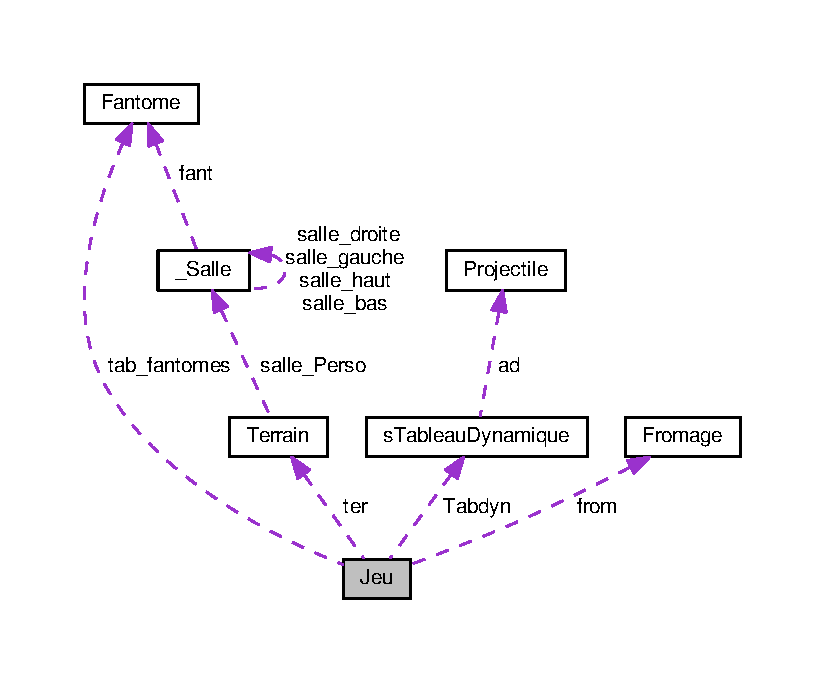
\includegraphics[width=350pt]{struct_jeu__coll__graph}
\end{center}
\end{figure}
\subsection*{Data Fields}
\begin{DoxyCompactItemize}
\item 
\hyperlink{struct_terrain}{Terrain} \hyperlink{struct_jeu_ad8002797870fb7f9118f158aa1cba297}{ter}
\item 
\hyperlink{struct_fromage}{Fromage} \hyperlink{struct_jeu_ad750813cc55d2f02672d8197594350d4}{from}
\item 
\hyperlink{struct_fantome}{Fantome} $\ast$ \hyperlink{struct_jeu_aacb99c7d77e7b2be482dbf4be9d7f7cd}{tab\-\_\-fantomes}
\item 
int \hyperlink{struct_jeu_a2af79f2e5c4d4e38523422de3a02f380}{nb\-\_\-fantomes}
\item 
\hyperlink{_jeu_8h_a8248fdbab1c5aa4232c53c2f209f989a}{Tableau\-Dynamique} \hyperlink{struct_jeu_ac3c24a0cc9b72986a66bd7cd89c36b98}{Tabdyn}
\end{DoxyCompactItemize}


\subsection{Detailed Description}


Definition at line 21 of file Jeu.\-h.



\subsection{Field Documentation}
\hypertarget{struct_jeu_ad750813cc55d2f02672d8197594350d4}{\index{Jeu@{Jeu}!from@{from}}
\index{from@{from}!Jeu@{Jeu}}
\subsubsection[{from}]{\setlength{\rightskip}{0pt plus 5cm}{\bf Fromage} from}}\label{struct_jeu_ad750813cc55d2f02672d8197594350d4}


Definition at line 24 of file Jeu.\-h.

\hypertarget{struct_jeu_a2af79f2e5c4d4e38523422de3a02f380}{\index{Jeu@{Jeu}!nb\-\_\-fantomes@{nb\-\_\-fantomes}}
\index{nb\-\_\-fantomes@{nb\-\_\-fantomes}!Jeu@{Jeu}}
\subsubsection[{nb\-\_\-fantomes}]{\setlength{\rightskip}{0pt plus 5cm}int nb\-\_\-fantomes}}\label{struct_jeu_a2af79f2e5c4d4e38523422de3a02f380}


Definition at line 26 of file Jeu.\-h.

\hypertarget{struct_jeu_aacb99c7d77e7b2be482dbf4be9d7f7cd}{\index{Jeu@{Jeu}!tab\-\_\-fantomes@{tab\-\_\-fantomes}}
\index{tab\-\_\-fantomes@{tab\-\_\-fantomes}!Jeu@{Jeu}}
\subsubsection[{tab\-\_\-fantomes}]{\setlength{\rightskip}{0pt plus 5cm}{\bf Fantome}$\ast$ tab\-\_\-fantomes}}\label{struct_jeu_aacb99c7d77e7b2be482dbf4be9d7f7cd}


Definition at line 25 of file Jeu.\-h.

\hypertarget{struct_jeu_ac3c24a0cc9b72986a66bd7cd89c36b98}{\index{Jeu@{Jeu}!Tabdyn@{Tabdyn}}
\index{Tabdyn@{Tabdyn}!Jeu@{Jeu}}
\subsubsection[{Tabdyn}]{\setlength{\rightskip}{0pt plus 5cm}{\bf Tableau\-Dynamique} Tabdyn}}\label{struct_jeu_ac3c24a0cc9b72986a66bd7cd89c36b98}


Definition at line 27 of file Jeu.\-h.

\hypertarget{struct_jeu_ad8002797870fb7f9118f158aa1cba297}{\index{Jeu@{Jeu}!ter@{ter}}
\index{ter@{ter}!Jeu@{Jeu}}
\subsubsection[{ter}]{\setlength{\rightskip}{0pt plus 5cm}{\bf Terrain} ter}}\label{struct_jeu_ad8002797870fb7f9118f158aa1cba297}


Definition at line 23 of file Jeu.\-h.



The documentation for this struct was generated from the following file\-:\begin{DoxyCompactItemize}
\item 
/home/enzo/projet\-\_\-fluide/src/\hyperlink{_jeu_8h}{Jeu.\-h}\end{DoxyCompactItemize}

\hypertarget{struct_projectile}{\section{Projectile Struct Reference}
\label{struct_projectile}\index{Projectile@{Projectile}}
}


{\ttfamily \#include $<$Jeu.\-h$>$}

\subsection*{Data Fields}
\begin{DoxyCompactItemize}
\item 
int \hyperlink{struct_projectile_a6150e0515f7202e2fb518f7206ed97dc}{x}
\item 
int \hyperlink{struct_projectile_a0a2f84ed7838f07779ae24c5a9086d33}{y}
\item 
int \hyperlink{struct_projectile_a528d22a2a1651a4831eb643884a3c718}{orientation}
\item 
int \hyperlink{struct_projectile_a48cb20b0f4b6246bb181b3633e3c3f89}{tir\-From}
\end{DoxyCompactItemize}


\subsection{Detailed Description}


Definition at line 6 of file Jeu.\-h.



\subsection{Field Documentation}
\hypertarget{struct_projectile_a528d22a2a1651a4831eb643884a3c718}{\index{Projectile@{Projectile}!orientation@{orientation}}
\index{orientation@{orientation}!Projectile@{Projectile}}
\subsubsection[{orientation}]{\setlength{\rightskip}{0pt plus 5cm}int orientation}}\label{struct_projectile_a528d22a2a1651a4831eb643884a3c718}


Definition at line 8 of file Jeu.\-h.

\hypertarget{struct_projectile_a48cb20b0f4b6246bb181b3633e3c3f89}{\index{Projectile@{Projectile}!tir\-From@{tir\-From}}
\index{tir\-From@{tir\-From}!Projectile@{Projectile}}
\subsubsection[{tir\-From}]{\setlength{\rightskip}{0pt plus 5cm}int tir\-From}}\label{struct_projectile_a48cb20b0f4b6246bb181b3633e3c3f89}


Definition at line 8 of file Jeu.\-h.

\hypertarget{struct_projectile_a6150e0515f7202e2fb518f7206ed97dc}{\index{Projectile@{Projectile}!x@{x}}
\index{x@{x}!Projectile@{Projectile}}
\subsubsection[{x}]{\setlength{\rightskip}{0pt plus 5cm}int x}}\label{struct_projectile_a6150e0515f7202e2fb518f7206ed97dc}


Definition at line 8 of file Jeu.\-h.

\hypertarget{struct_projectile_a0a2f84ed7838f07779ae24c5a9086d33}{\index{Projectile@{Projectile}!y@{y}}
\index{y@{y}!Projectile@{Projectile}}
\subsubsection[{y}]{\setlength{\rightskip}{0pt plus 5cm}int y}}\label{struct_projectile_a0a2f84ed7838f07779ae24c5a9086d33}


Definition at line 8 of file Jeu.\-h.



The documentation for this struct was generated from the following file\-:\begin{DoxyCompactItemize}
\item 
/home/enzo/projet\-\_\-fluide/src/\hyperlink{_jeu_8h}{Jeu.\-h}\end{DoxyCompactItemize}

\hypertarget{structsdl_jeu}{\section{sdl\-Jeu Struct Reference}
\label{structsdl_jeu}\index{sdl\-Jeu@{sdl\-Jeu}}
}


{\ttfamily \#include $<$sdl\-Jeu.\-h$>$}



Collaboration diagram for sdl\-Jeu\-:\nopagebreak
\begin{figure}[H]
\begin{center}
\leavevmode
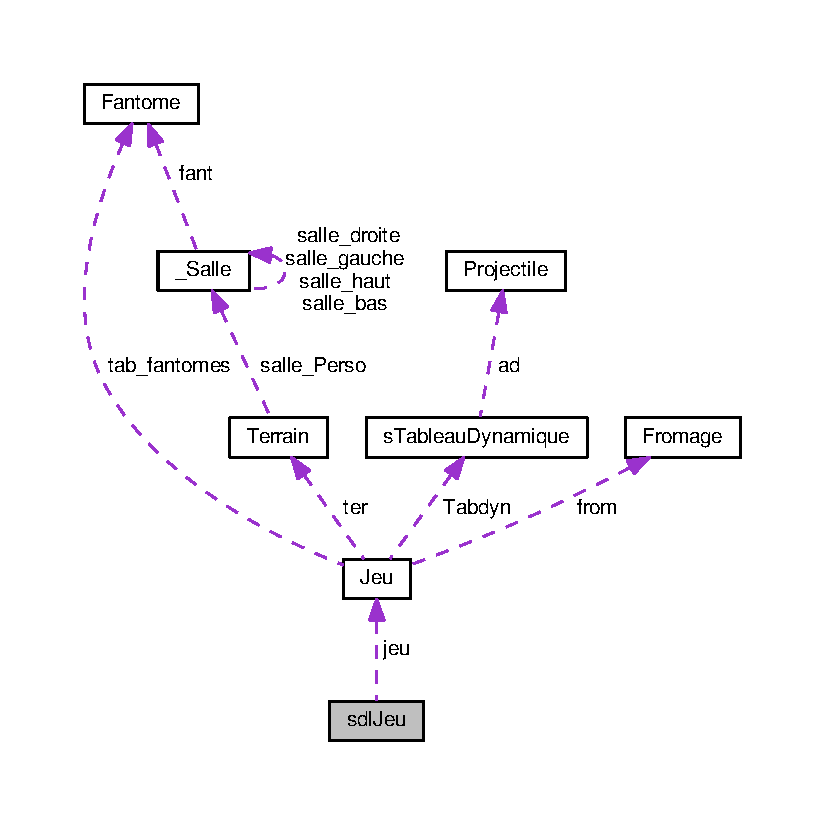
\includegraphics[width=350pt]{structsdl_jeu__coll__graph}
\end{center}
\end{figure}
\subsection*{Data Fields}
\begin{DoxyCompactItemize}
\item 
int \hyperlink{structsdl_jeu_a52e5e34765d5dbac15d959dbaddf4e5e}{jeu\-O\-N}
\item 
\hyperlink{struct_jeu}{Jeu} \hyperlink{structsdl_jeu_a56ca1ac56f66324ba9bc5868128ddb84}{jeu}
\item 
S\-D\-L\-\_\-\-Surface $\ast$ \hyperlink{structsdl_jeu_a3970583cd7133d59e68d97fc4023ab99}{surface\-\_\-ecran}
\item 
S\-D\-L\-\_\-\-Surface $\ast$ \hyperlink{structsdl_jeu_afd00ed4bfd7c3861399353daf3448bdf}{surface\-\_\-fromage\-\_\-gauche}
\item 
S\-D\-L\-\_\-\-Surface $\ast$ \hyperlink{structsdl_jeu_a7c6ef35a42794f835aa8b46035ee47fa}{surface\-\_\-fromage\-\_\-droite}
\item 
S\-D\-L\-\_\-\-Surface $\ast$ \hyperlink{structsdl_jeu_a71c9d3841b956efd1679703045750d21}{surface\-\_\-fromage\-\_\-droite1}
\item 
S\-D\-L\-\_\-\-Surface $\ast$ \hyperlink{structsdl_jeu_adfb16227a11193bf81b7781d3e39589a}{surface\-\_\-fromage\-\_\-gauche1}
\item 
S\-D\-L\-\_\-\-Surface $\ast$ \hyperlink{structsdl_jeu_abfef78dde33045acb50cc005888ef184}{surface\-\_\-fromage\-\_\-saut}
\item 
S\-D\-L\-\_\-\-Surface $\ast$ \hyperlink{structsdl_jeu_a4725423b3638295a6ecc002c96826235}{surface\-\_\-fromage\-\_\-tir}
\item 
S\-D\-L\-\_\-\-Surface $\ast$ \hyperlink{structsdl_jeu_ae7b0c7c4f3c21bed15109564ca380a64}{surface\-\_\-fromage\-\_\-mort\-\_\-droite}
\item 
S\-D\-L\-\_\-\-Surface $\ast$ \hyperlink{structsdl_jeu_ab0f132d65433e47f88112b705dc1b3cb}{surface\-\_\-fromage\-\_\-mort\-\_\-gauche}
\item 
S\-D\-L\-\_\-\-Surface $\ast$ \hyperlink{structsdl_jeu_af661b67f0b78d8093091c652a6bc0bbc}{surface\-\_\-fromage\-\_\-saut\-\_\-tir}
\item 
S\-D\-L\-\_\-\-Surface $\ast$ \hyperlink{structsdl_jeu_a1eae6cdffcfd9a581314a0377e25b825}{surface\-\_\-mur}
\item 
S\-D\-L\-\_\-\-Surface $\ast$ \hyperlink{structsdl_jeu_afff984367bbdf019fda00ae1d3e8a8d6}{surface\-\_\-fantome}
\item 
S\-D\-L\-\_\-\-Surface $\ast$ \hyperlink{structsdl_jeu_a63e27a4ffca9b9d744f1c59ccceccfee}{surface\-\_\-fantome\-\_\-mort\-\_\-droite}
\item 
S\-D\-L\-\_\-\-Surface $\ast$ \hyperlink{structsdl_jeu_ad05a5d488af4b9304bd3a918bf03c699}{surface\-\_\-fantome\-\_\-mort\-\_\-gauche}
\item 
S\-D\-L\-\_\-\-Surface $\ast$ \hyperlink{structsdl_jeu_a0421d88f322a7e945216dacac7b0821e}{surface\-\_\-porte}
\item 
S\-D\-L\-\_\-\-Surface $\ast$ \hyperlink{structsdl_jeu_a9f68bf316a2241185e3c8f8b3d038d85}{surface\-\_\-hp}
\item 
S\-D\-L\-\_\-\-Surface $\ast$ \hyperlink{structsdl_jeu_aa4f79a6d22df2ec6768024e745708e2b}{fond\-\_\-base}
\item 
S\-D\-L\-\_\-\-Surface $\ast$ \hyperlink{structsdl_jeu_a85ab02081c98d07a898482a21e48b56e}{fond\-\_\-sombre}
\item 
S\-D\-L\-\_\-\-Surface $\ast$ \hyperlink{structsdl_jeu_a9fe0fcc6750250a9b4ed6c34c6ac18d2}{sol}
\item 
S\-D\-L\-\_\-\-Surface $\ast$ \hyperlink{structsdl_jeu_a18302ff4ecbc30500bf2638c3036aa8d}{lumiere}
\item 
S\-D\-L\-\_\-\-Surface $\ast$ \hyperlink{structsdl_jeu_a96eebd19c7cea6af7e50e821d04ed494}{fenetre}
\item 
S\-D\-L\-\_\-\-Surface $\ast$ \hyperlink{structsdl_jeu_a0a838f8347a9ea3ab071107815325988}{gandalf}
\item 
S\-D\-L\-\_\-\-Surface $\ast$ \hyperlink{structsdl_jeu_a761714fd2e059e5f8b4e0a5246f0413f}{pic}
\item 
S\-D\-L\-\_\-\-Surface $\ast$ \hyperlink{structsdl_jeu_af901fa03839c9ce73b3a49a79e5a417e}{projo\-\_\-gauche}
\item 
S\-D\-L\-\_\-\-Surface $\ast$ \hyperlink{structsdl_jeu_a18c766351a8d4a2399cde76a7d894559}{projo\-\_\-haut}
\item 
S\-D\-L\-\_\-\-Surface $\ast$ \hyperlink{structsdl_jeu_a057caebe9a2bda0166b2767d19d84318}{projo\-\_\-bas}
\item 
S\-D\-L\-\_\-\-Surface $\ast$ \hyperlink{structsdl_jeu_a752f2ccb603dfdb70f4d2da72fb5ccc5}{projo\-\_\-droite}
\item 
S\-D\-L\-\_\-\-Surface $\ast$ \hyperlink{structsdl_jeu_a5d1c1a5b6d8f7dd5b4f69871198f36b9}{surface\-\_\-clef}
\item 
S\-D\-L\-\_\-\-Surface $\ast$ \hyperlink{structsdl_jeu_a319f836c1aeb2c6308e8787e7c19977f}{projo\-\_\-blue\-\_\-gauche}
\item 
S\-D\-L\-\_\-\-Surface $\ast$ \hyperlink{structsdl_jeu_a199f1dad5defaafc584de63f511c9016}{projo\-\_\-blue\-\_\-haut}
\item 
S\-D\-L\-\_\-\-Surface $\ast$ \hyperlink{structsdl_jeu_a8798b282fc596b5711ba522d95ffb041}{projo\-\_\-blue\-\_\-bas}
\item 
S\-D\-L\-\_\-\-Surface $\ast$ \hyperlink{structsdl_jeu_af18510332136243335ab74b8f6876e1d}{projo\-\_\-blue\-\_\-droite}
\item 
S\-D\-L\-\_\-\-Surface $\ast$ \hyperlink{structsdl_jeu_af673014bd91e1e646926754799ab18d0}{surface\-\_\-fond}
\item 
S\-D\-L\-\_\-\-Surface $\ast$ \hyperlink{structsdl_jeu_a29c6542f0f27a5c7d75584b0332818b1}{surface\-\_\-menu}
\item 
S\-D\-L\-\_\-\-Surface $\ast$ \hyperlink{structsdl_jeu_a064aa3c5aa4bb35c72af2e7ec4af4722}{bouton\-\_\-menu\-\_\-1}
\item 
S\-D\-L\-\_\-\-Surface $\ast$ \hyperlink{structsdl_jeu_a529025a491485aef1616d286edff9ae7}{bouton\-\_\-menu\-\_\-2}
\item 
S\-D\-L\-\_\-\-Surface $\ast$ \hyperlink{structsdl_jeu_ad38d5f8cc0767da2a95b809b7ec5aa56}{bouton\-\_\-menu\-\_\-3}
\item 
S\-D\-L\-\_\-\-Rect \hyperlink{structsdl_jeu_a1bb4e9da2e503d2e0c61d362a5e13234}{pos\-Fond}
\item 
S\-D\-L\-\_\-\-Rect \hyperlink{structsdl_jeu_a61a141b7f826f13b1a404bac31aabe4c}{Fond}
\item 
S\-D\-L\-\_\-\-Rect \hyperlink{structsdl_jeu_af6051c9f489b13415829103eab2689af}{pos\-Bouton1}
\item 
S\-D\-L\-\_\-\-Rect \hyperlink{structsdl_jeu_a23f4550911b88a484d4530c86026c191}{pos\-Bouton2}
\item 
S\-D\-L\-\_\-\-Rect \hyperlink{structsdl_jeu_a9e93c0144eeff3329f7a5ee934eca81d}{pos\-Bouton3}
\item 
Mix\-\_\-\-Music $\ast$ \hyperlink{structsdl_jeu_af7321948c26bf773e1bbee605d15c2d7}{main\-\_\-theme}
\item 
Mix\-\_\-\-Music $\ast$ \hyperlink{structsdl_jeu_af21ea3aee1c3c164e57edddad03634fe}{menu\-\_\-theme}
\item 
Mix\-\_\-\-Chunk $\ast$ \hyperlink{structsdl_jeu_ac3dc104264d31879f76daa8cb4c61bca}{laser1}
\item 
Mix\-\_\-\-Chunk $\ast$ \hyperlink{structsdl_jeu_a4dc97c9681105e31fd50f5cc1d4db7fa}{son\-\_\-mort}
\item 
Mix\-\_\-\-Chunk $\ast$ \hyperlink{structsdl_jeu_a58f8eda8c295fc531edf99fb867053a8}{bip\-\_\-menu}
\end{DoxyCompactItemize}


\subsection{Detailed Description}


Definition at line 15 of file sdl\-Jeu.\-h.



\subsection{Field Documentation}
\hypertarget{structsdl_jeu_a58f8eda8c295fc531edf99fb867053a8}{\index{sdl\-Jeu@{sdl\-Jeu}!bip\-\_\-menu@{bip\-\_\-menu}}
\index{bip\-\_\-menu@{bip\-\_\-menu}!sdlJeu@{sdl\-Jeu}}
\subsubsection[{bip\-\_\-menu}]{\setlength{\rightskip}{0pt plus 5cm}Mix\-\_\-\-Chunk$\ast$ bip\-\_\-menu}}\label{structsdl_jeu_a58f8eda8c295fc531edf99fb867053a8}


Definition at line 77 of file sdl\-Jeu.\-h.

\hypertarget{structsdl_jeu_a064aa3c5aa4bb35c72af2e7ec4af4722}{\index{sdl\-Jeu@{sdl\-Jeu}!bouton\-\_\-menu\-\_\-1@{bouton\-\_\-menu\-\_\-1}}
\index{bouton\-\_\-menu\-\_\-1@{bouton\-\_\-menu\-\_\-1}!sdlJeu@{sdl\-Jeu}}
\subsubsection[{bouton\-\_\-menu\-\_\-1}]{\setlength{\rightskip}{0pt plus 5cm}S\-D\-L\-\_\-\-Surface$\ast$ bouton\-\_\-menu\-\_\-1}}\label{structsdl_jeu_a064aa3c5aa4bb35c72af2e7ec4af4722}


Definition at line 63 of file sdl\-Jeu.\-h.

\hypertarget{structsdl_jeu_a529025a491485aef1616d286edff9ae7}{\index{sdl\-Jeu@{sdl\-Jeu}!bouton\-\_\-menu\-\_\-2@{bouton\-\_\-menu\-\_\-2}}
\index{bouton\-\_\-menu\-\_\-2@{bouton\-\_\-menu\-\_\-2}!sdlJeu@{sdl\-Jeu}}
\subsubsection[{bouton\-\_\-menu\-\_\-2}]{\setlength{\rightskip}{0pt plus 5cm}S\-D\-L\-\_\-\-Surface$\ast$ bouton\-\_\-menu\-\_\-2}}\label{structsdl_jeu_a529025a491485aef1616d286edff9ae7}


Definition at line 64 of file sdl\-Jeu.\-h.

\hypertarget{structsdl_jeu_ad38d5f8cc0767da2a95b809b7ec5aa56}{\index{sdl\-Jeu@{sdl\-Jeu}!bouton\-\_\-menu\-\_\-3@{bouton\-\_\-menu\-\_\-3}}
\index{bouton\-\_\-menu\-\_\-3@{bouton\-\_\-menu\-\_\-3}!sdlJeu@{sdl\-Jeu}}
\subsubsection[{bouton\-\_\-menu\-\_\-3}]{\setlength{\rightskip}{0pt plus 5cm}S\-D\-L\-\_\-\-Surface$\ast$ bouton\-\_\-menu\-\_\-3}}\label{structsdl_jeu_ad38d5f8cc0767da2a95b809b7ec5aa56}


Definition at line 65 of file sdl\-Jeu.\-h.

\hypertarget{structsdl_jeu_a96eebd19c7cea6af7e50e821d04ed494}{\index{sdl\-Jeu@{sdl\-Jeu}!fenetre@{fenetre}}
\index{fenetre@{fenetre}!sdlJeu@{sdl\-Jeu}}
\subsubsection[{fenetre}]{\setlength{\rightskip}{0pt plus 5cm}S\-D\-L\-\_\-\-Surface$\ast$ fenetre}}\label{structsdl_jeu_a96eebd19c7cea6af7e50e821d04ed494}


Definition at line 46 of file sdl\-Jeu.\-h.

\hypertarget{structsdl_jeu_a61a141b7f826f13b1a404bac31aabe4c}{\index{sdl\-Jeu@{sdl\-Jeu}!Fond@{Fond}}
\index{Fond@{Fond}!sdlJeu@{sdl\-Jeu}}
\subsubsection[{Fond}]{\setlength{\rightskip}{0pt plus 5cm}S\-D\-L\-\_\-\-Rect Fond}}\label{structsdl_jeu_a61a141b7f826f13b1a404bac31aabe4c}


Definition at line 68 of file sdl\-Jeu.\-h.

\hypertarget{structsdl_jeu_aa4f79a6d22df2ec6768024e745708e2b}{\index{sdl\-Jeu@{sdl\-Jeu}!fond\-\_\-base@{fond\-\_\-base}}
\index{fond\-\_\-base@{fond\-\_\-base}!sdlJeu@{sdl\-Jeu}}
\subsubsection[{fond\-\_\-base}]{\setlength{\rightskip}{0pt plus 5cm}S\-D\-L\-\_\-\-Surface$\ast$ fond\-\_\-base}}\label{structsdl_jeu_aa4f79a6d22df2ec6768024e745708e2b}


Definition at line 42 of file sdl\-Jeu.\-h.

\hypertarget{structsdl_jeu_a85ab02081c98d07a898482a21e48b56e}{\index{sdl\-Jeu@{sdl\-Jeu}!fond\-\_\-sombre@{fond\-\_\-sombre}}
\index{fond\-\_\-sombre@{fond\-\_\-sombre}!sdlJeu@{sdl\-Jeu}}
\subsubsection[{fond\-\_\-sombre}]{\setlength{\rightskip}{0pt plus 5cm}S\-D\-L\-\_\-\-Surface$\ast$ fond\-\_\-sombre}}\label{structsdl_jeu_a85ab02081c98d07a898482a21e48b56e}


Definition at line 43 of file sdl\-Jeu.\-h.

\hypertarget{structsdl_jeu_a0a838f8347a9ea3ab071107815325988}{\index{sdl\-Jeu@{sdl\-Jeu}!gandalf@{gandalf}}
\index{gandalf@{gandalf}!sdlJeu@{sdl\-Jeu}}
\subsubsection[{gandalf}]{\setlength{\rightskip}{0pt plus 5cm}S\-D\-L\-\_\-\-Surface$\ast$ gandalf}}\label{structsdl_jeu_a0a838f8347a9ea3ab071107815325988}


Definition at line 47 of file sdl\-Jeu.\-h.

\hypertarget{structsdl_jeu_a56ca1ac56f66324ba9bc5868128ddb84}{\index{sdl\-Jeu@{sdl\-Jeu}!jeu@{jeu}}
\index{jeu@{jeu}!sdlJeu@{sdl\-Jeu}}
\subsubsection[{jeu}]{\setlength{\rightskip}{0pt plus 5cm}{\bf Jeu} jeu}}\label{structsdl_jeu_a56ca1ac56f66324ba9bc5868128ddb84}


Definition at line 18 of file sdl\-Jeu.\-h.

\hypertarget{structsdl_jeu_a52e5e34765d5dbac15d959dbaddf4e5e}{\index{sdl\-Jeu@{sdl\-Jeu}!jeu\-O\-N@{jeu\-O\-N}}
\index{jeu\-O\-N@{jeu\-O\-N}!sdlJeu@{sdl\-Jeu}}
\subsubsection[{jeu\-O\-N}]{\setlength{\rightskip}{0pt plus 5cm}int jeu\-O\-N}}\label{structsdl_jeu_a52e5e34765d5dbac15d959dbaddf4e5e}


Definition at line 17 of file sdl\-Jeu.\-h.

\hypertarget{structsdl_jeu_ac3dc104264d31879f76daa8cb4c61bca}{\index{sdl\-Jeu@{sdl\-Jeu}!laser1@{laser1}}
\index{laser1@{laser1}!sdlJeu@{sdl\-Jeu}}
\subsubsection[{laser1}]{\setlength{\rightskip}{0pt plus 5cm}Mix\-\_\-\-Chunk$\ast$ laser1}}\label{structsdl_jeu_ac3dc104264d31879f76daa8cb4c61bca}


Definition at line 75 of file sdl\-Jeu.\-h.

\hypertarget{structsdl_jeu_a18302ff4ecbc30500bf2638c3036aa8d}{\index{sdl\-Jeu@{sdl\-Jeu}!lumiere@{lumiere}}
\index{lumiere@{lumiere}!sdlJeu@{sdl\-Jeu}}
\subsubsection[{lumiere}]{\setlength{\rightskip}{0pt plus 5cm}S\-D\-L\-\_\-\-Surface$\ast$ lumiere}}\label{structsdl_jeu_a18302ff4ecbc30500bf2638c3036aa8d}


Definition at line 45 of file sdl\-Jeu.\-h.

\hypertarget{structsdl_jeu_af7321948c26bf773e1bbee605d15c2d7}{\index{sdl\-Jeu@{sdl\-Jeu}!main\-\_\-theme@{main\-\_\-theme}}
\index{main\-\_\-theme@{main\-\_\-theme}!sdlJeu@{sdl\-Jeu}}
\subsubsection[{main\-\_\-theme}]{\setlength{\rightskip}{0pt plus 5cm}Mix\-\_\-\-Music$\ast$ main\-\_\-theme}}\label{structsdl_jeu_af7321948c26bf773e1bbee605d15c2d7}


Definition at line 73 of file sdl\-Jeu.\-h.

\hypertarget{structsdl_jeu_af21ea3aee1c3c164e57edddad03634fe}{\index{sdl\-Jeu@{sdl\-Jeu}!menu\-\_\-theme@{menu\-\_\-theme}}
\index{menu\-\_\-theme@{menu\-\_\-theme}!sdlJeu@{sdl\-Jeu}}
\subsubsection[{menu\-\_\-theme}]{\setlength{\rightskip}{0pt plus 5cm}Mix\-\_\-\-Music$\ast$ menu\-\_\-theme}}\label{structsdl_jeu_af21ea3aee1c3c164e57edddad03634fe}


Definition at line 74 of file sdl\-Jeu.\-h.

\hypertarget{structsdl_jeu_a761714fd2e059e5f8b4e0a5246f0413f}{\index{sdl\-Jeu@{sdl\-Jeu}!pic@{pic}}
\index{pic@{pic}!sdlJeu@{sdl\-Jeu}}
\subsubsection[{pic}]{\setlength{\rightskip}{0pt plus 5cm}S\-D\-L\-\_\-\-Surface$\ast$ pic}}\label{structsdl_jeu_a761714fd2e059e5f8b4e0a5246f0413f}


Definition at line 48 of file sdl\-Jeu.\-h.

\hypertarget{structsdl_jeu_af6051c9f489b13415829103eab2689af}{\index{sdl\-Jeu@{sdl\-Jeu}!pos\-Bouton1@{pos\-Bouton1}}
\index{pos\-Bouton1@{pos\-Bouton1}!sdlJeu@{sdl\-Jeu}}
\subsubsection[{pos\-Bouton1}]{\setlength{\rightskip}{0pt plus 5cm}S\-D\-L\-\_\-\-Rect pos\-Bouton1}}\label{structsdl_jeu_af6051c9f489b13415829103eab2689af}


Definition at line 69 of file sdl\-Jeu.\-h.

\hypertarget{structsdl_jeu_a23f4550911b88a484d4530c86026c191}{\index{sdl\-Jeu@{sdl\-Jeu}!pos\-Bouton2@{pos\-Bouton2}}
\index{pos\-Bouton2@{pos\-Bouton2}!sdlJeu@{sdl\-Jeu}}
\subsubsection[{pos\-Bouton2}]{\setlength{\rightskip}{0pt plus 5cm}S\-D\-L\-\_\-\-Rect pos\-Bouton2}}\label{structsdl_jeu_a23f4550911b88a484d4530c86026c191}


Definition at line 70 of file sdl\-Jeu.\-h.

\hypertarget{structsdl_jeu_a9e93c0144eeff3329f7a5ee934eca81d}{\index{sdl\-Jeu@{sdl\-Jeu}!pos\-Bouton3@{pos\-Bouton3}}
\index{pos\-Bouton3@{pos\-Bouton3}!sdlJeu@{sdl\-Jeu}}
\subsubsection[{pos\-Bouton3}]{\setlength{\rightskip}{0pt plus 5cm}S\-D\-L\-\_\-\-Rect pos\-Bouton3}}\label{structsdl_jeu_a9e93c0144eeff3329f7a5ee934eca81d}


Definition at line 71 of file sdl\-Jeu.\-h.

\hypertarget{structsdl_jeu_a1bb4e9da2e503d2e0c61d362a5e13234}{\index{sdl\-Jeu@{sdl\-Jeu}!pos\-Fond@{pos\-Fond}}
\index{pos\-Fond@{pos\-Fond}!sdlJeu@{sdl\-Jeu}}
\subsubsection[{pos\-Fond}]{\setlength{\rightskip}{0pt plus 5cm}S\-D\-L\-\_\-\-Rect pos\-Fond}}\label{structsdl_jeu_a1bb4e9da2e503d2e0c61d362a5e13234}


Definition at line 67 of file sdl\-Jeu.\-h.

\hypertarget{structsdl_jeu_a057caebe9a2bda0166b2767d19d84318}{\index{sdl\-Jeu@{sdl\-Jeu}!projo\-\_\-bas@{projo\-\_\-bas}}
\index{projo\-\_\-bas@{projo\-\_\-bas}!sdlJeu@{sdl\-Jeu}}
\subsubsection[{projo\-\_\-bas}]{\setlength{\rightskip}{0pt plus 5cm}S\-D\-L\-\_\-\-Surface$\ast$ projo\-\_\-bas}}\label{structsdl_jeu_a057caebe9a2bda0166b2767d19d84318}


Definition at line 52 of file sdl\-Jeu.\-h.

\hypertarget{structsdl_jeu_a8798b282fc596b5711ba522d95ffb041}{\index{sdl\-Jeu@{sdl\-Jeu}!projo\-\_\-blue\-\_\-bas@{projo\-\_\-blue\-\_\-bas}}
\index{projo\-\_\-blue\-\_\-bas@{projo\-\_\-blue\-\_\-bas}!sdlJeu@{sdl\-Jeu}}
\subsubsection[{projo\-\_\-blue\-\_\-bas}]{\setlength{\rightskip}{0pt plus 5cm}S\-D\-L\-\_\-\-Surface$\ast$ projo\-\_\-blue\-\_\-bas}}\label{structsdl_jeu_a8798b282fc596b5711ba522d95ffb041}


Definition at line 58 of file sdl\-Jeu.\-h.

\hypertarget{structsdl_jeu_af18510332136243335ab74b8f6876e1d}{\index{sdl\-Jeu@{sdl\-Jeu}!projo\-\_\-blue\-\_\-droite@{projo\-\_\-blue\-\_\-droite}}
\index{projo\-\_\-blue\-\_\-droite@{projo\-\_\-blue\-\_\-droite}!sdlJeu@{sdl\-Jeu}}
\subsubsection[{projo\-\_\-blue\-\_\-droite}]{\setlength{\rightskip}{0pt plus 5cm}S\-D\-L\-\_\-\-Surface$\ast$ projo\-\_\-blue\-\_\-droite}}\label{structsdl_jeu_af18510332136243335ab74b8f6876e1d}


Definition at line 59 of file sdl\-Jeu.\-h.

\hypertarget{structsdl_jeu_a319f836c1aeb2c6308e8787e7c19977f}{\index{sdl\-Jeu@{sdl\-Jeu}!projo\-\_\-blue\-\_\-gauche@{projo\-\_\-blue\-\_\-gauche}}
\index{projo\-\_\-blue\-\_\-gauche@{projo\-\_\-blue\-\_\-gauche}!sdlJeu@{sdl\-Jeu}}
\subsubsection[{projo\-\_\-blue\-\_\-gauche}]{\setlength{\rightskip}{0pt plus 5cm}S\-D\-L\-\_\-\-Surface$\ast$ projo\-\_\-blue\-\_\-gauche}}\label{structsdl_jeu_a319f836c1aeb2c6308e8787e7c19977f}


Definition at line 56 of file sdl\-Jeu.\-h.

\hypertarget{structsdl_jeu_a199f1dad5defaafc584de63f511c9016}{\index{sdl\-Jeu@{sdl\-Jeu}!projo\-\_\-blue\-\_\-haut@{projo\-\_\-blue\-\_\-haut}}
\index{projo\-\_\-blue\-\_\-haut@{projo\-\_\-blue\-\_\-haut}!sdlJeu@{sdl\-Jeu}}
\subsubsection[{projo\-\_\-blue\-\_\-haut}]{\setlength{\rightskip}{0pt plus 5cm}S\-D\-L\-\_\-\-Surface$\ast$ projo\-\_\-blue\-\_\-haut}}\label{structsdl_jeu_a199f1dad5defaafc584de63f511c9016}


Definition at line 57 of file sdl\-Jeu.\-h.

\hypertarget{structsdl_jeu_a752f2ccb603dfdb70f4d2da72fb5ccc5}{\index{sdl\-Jeu@{sdl\-Jeu}!projo\-\_\-droite@{projo\-\_\-droite}}
\index{projo\-\_\-droite@{projo\-\_\-droite}!sdlJeu@{sdl\-Jeu}}
\subsubsection[{projo\-\_\-droite}]{\setlength{\rightskip}{0pt plus 5cm}S\-D\-L\-\_\-\-Surface$\ast$ projo\-\_\-droite}}\label{structsdl_jeu_a752f2ccb603dfdb70f4d2da72fb5ccc5}


Definition at line 53 of file sdl\-Jeu.\-h.

\hypertarget{structsdl_jeu_af901fa03839c9ce73b3a49a79e5a417e}{\index{sdl\-Jeu@{sdl\-Jeu}!projo\-\_\-gauche@{projo\-\_\-gauche}}
\index{projo\-\_\-gauche@{projo\-\_\-gauche}!sdlJeu@{sdl\-Jeu}}
\subsubsection[{projo\-\_\-gauche}]{\setlength{\rightskip}{0pt plus 5cm}S\-D\-L\-\_\-\-Surface$\ast$ projo\-\_\-gauche}}\label{structsdl_jeu_af901fa03839c9ce73b3a49a79e5a417e}


Definition at line 50 of file sdl\-Jeu.\-h.

\hypertarget{structsdl_jeu_a18c766351a8d4a2399cde76a7d894559}{\index{sdl\-Jeu@{sdl\-Jeu}!projo\-\_\-haut@{projo\-\_\-haut}}
\index{projo\-\_\-haut@{projo\-\_\-haut}!sdlJeu@{sdl\-Jeu}}
\subsubsection[{projo\-\_\-haut}]{\setlength{\rightskip}{0pt plus 5cm}S\-D\-L\-\_\-\-Surface$\ast$ projo\-\_\-haut}}\label{structsdl_jeu_a18c766351a8d4a2399cde76a7d894559}


Definition at line 51 of file sdl\-Jeu.\-h.

\hypertarget{structsdl_jeu_a9fe0fcc6750250a9b4ed6c34c6ac18d2}{\index{sdl\-Jeu@{sdl\-Jeu}!sol@{sol}}
\index{sol@{sol}!sdlJeu@{sdl\-Jeu}}
\subsubsection[{sol}]{\setlength{\rightskip}{0pt plus 5cm}S\-D\-L\-\_\-\-Surface$\ast$ sol}}\label{structsdl_jeu_a9fe0fcc6750250a9b4ed6c34c6ac18d2}


Definition at line 44 of file sdl\-Jeu.\-h.

\hypertarget{structsdl_jeu_a4dc97c9681105e31fd50f5cc1d4db7fa}{\index{sdl\-Jeu@{sdl\-Jeu}!son\-\_\-mort@{son\-\_\-mort}}
\index{son\-\_\-mort@{son\-\_\-mort}!sdlJeu@{sdl\-Jeu}}
\subsubsection[{son\-\_\-mort}]{\setlength{\rightskip}{0pt plus 5cm}Mix\-\_\-\-Chunk$\ast$ son\-\_\-mort}}\label{structsdl_jeu_a4dc97c9681105e31fd50f5cc1d4db7fa}


Definition at line 76 of file sdl\-Jeu.\-h.

\hypertarget{structsdl_jeu_a5d1c1a5b6d8f7dd5b4f69871198f36b9}{\index{sdl\-Jeu@{sdl\-Jeu}!surface\-\_\-clef@{surface\-\_\-clef}}
\index{surface\-\_\-clef@{surface\-\_\-clef}!sdlJeu@{sdl\-Jeu}}
\subsubsection[{surface\-\_\-clef}]{\setlength{\rightskip}{0pt plus 5cm}S\-D\-L\-\_\-\-Surface$\ast$ surface\-\_\-clef}}\label{structsdl_jeu_a5d1c1a5b6d8f7dd5b4f69871198f36b9}


Definition at line 54 of file sdl\-Jeu.\-h.

\hypertarget{structsdl_jeu_a3970583cd7133d59e68d97fc4023ab99}{\index{sdl\-Jeu@{sdl\-Jeu}!surface\-\_\-ecran@{surface\-\_\-ecran}}
\index{surface\-\_\-ecran@{surface\-\_\-ecran}!sdlJeu@{sdl\-Jeu}}
\subsubsection[{surface\-\_\-ecran}]{\setlength{\rightskip}{0pt plus 5cm}S\-D\-L\-\_\-\-Surface$\ast$ surface\-\_\-ecran}}\label{structsdl_jeu_a3970583cd7133d59e68d97fc4023ab99}


Definition at line 19 of file sdl\-Jeu.\-h.

\hypertarget{structsdl_jeu_afff984367bbdf019fda00ae1d3e8a8d6}{\index{sdl\-Jeu@{sdl\-Jeu}!surface\-\_\-fantome@{surface\-\_\-fantome}}
\index{surface\-\_\-fantome@{surface\-\_\-fantome}!sdlJeu@{sdl\-Jeu}}
\subsubsection[{surface\-\_\-fantome}]{\setlength{\rightskip}{0pt plus 5cm}S\-D\-L\-\_\-\-Surface$\ast$ surface\-\_\-fantome}}\label{structsdl_jeu_afff984367bbdf019fda00ae1d3e8a8d6}


Definition at line 37 of file sdl\-Jeu.\-h.

\hypertarget{structsdl_jeu_a63e27a4ffca9b9d744f1c59ccceccfee}{\index{sdl\-Jeu@{sdl\-Jeu}!surface\-\_\-fantome\-\_\-mort\-\_\-droite@{surface\-\_\-fantome\-\_\-mort\-\_\-droite}}
\index{surface\-\_\-fantome\-\_\-mort\-\_\-droite@{surface\-\_\-fantome\-\_\-mort\-\_\-droite}!sdlJeu@{sdl\-Jeu}}
\subsubsection[{surface\-\_\-fantome\-\_\-mort\-\_\-droite}]{\setlength{\rightskip}{0pt plus 5cm}S\-D\-L\-\_\-\-Surface$\ast$ surface\-\_\-fantome\-\_\-mort\-\_\-droite}}\label{structsdl_jeu_a63e27a4ffca9b9d744f1c59ccceccfee}


Definition at line 38 of file sdl\-Jeu.\-h.

\hypertarget{structsdl_jeu_ad05a5d488af4b9304bd3a918bf03c699}{\index{sdl\-Jeu@{sdl\-Jeu}!surface\-\_\-fantome\-\_\-mort\-\_\-gauche@{surface\-\_\-fantome\-\_\-mort\-\_\-gauche}}
\index{surface\-\_\-fantome\-\_\-mort\-\_\-gauche@{surface\-\_\-fantome\-\_\-mort\-\_\-gauche}!sdlJeu@{sdl\-Jeu}}
\subsubsection[{surface\-\_\-fantome\-\_\-mort\-\_\-gauche}]{\setlength{\rightskip}{0pt plus 5cm}S\-D\-L\-\_\-\-Surface$\ast$ surface\-\_\-fantome\-\_\-mort\-\_\-gauche}}\label{structsdl_jeu_ad05a5d488af4b9304bd3a918bf03c699}


Definition at line 39 of file sdl\-Jeu.\-h.

\hypertarget{structsdl_jeu_af673014bd91e1e646926754799ab18d0}{\index{sdl\-Jeu@{sdl\-Jeu}!surface\-\_\-fond@{surface\-\_\-fond}}
\index{surface\-\_\-fond@{surface\-\_\-fond}!sdlJeu@{sdl\-Jeu}}
\subsubsection[{surface\-\_\-fond}]{\setlength{\rightskip}{0pt plus 5cm}S\-D\-L\-\_\-\-Surface$\ast$ surface\-\_\-fond}}\label{structsdl_jeu_af673014bd91e1e646926754799ab18d0}


Definition at line 61 of file sdl\-Jeu.\-h.

\hypertarget{structsdl_jeu_a7c6ef35a42794f835aa8b46035ee47fa}{\index{sdl\-Jeu@{sdl\-Jeu}!surface\-\_\-fromage\-\_\-droite@{surface\-\_\-fromage\-\_\-droite}}
\index{surface\-\_\-fromage\-\_\-droite@{surface\-\_\-fromage\-\_\-droite}!sdlJeu@{sdl\-Jeu}}
\subsubsection[{surface\-\_\-fromage\-\_\-droite}]{\setlength{\rightskip}{0pt plus 5cm}S\-D\-L\-\_\-\-Surface$\ast$ surface\-\_\-fromage\-\_\-droite}}\label{structsdl_jeu_a7c6ef35a42794f835aa8b46035ee47fa}


Definition at line 21 of file sdl\-Jeu.\-h.

\hypertarget{structsdl_jeu_a71c9d3841b956efd1679703045750d21}{\index{sdl\-Jeu@{sdl\-Jeu}!surface\-\_\-fromage\-\_\-droite1@{surface\-\_\-fromage\-\_\-droite1}}
\index{surface\-\_\-fromage\-\_\-droite1@{surface\-\_\-fromage\-\_\-droite1}!sdlJeu@{sdl\-Jeu}}
\subsubsection[{surface\-\_\-fromage\-\_\-droite1}]{\setlength{\rightskip}{0pt plus 5cm}S\-D\-L\-\_\-\-Surface$\ast$ surface\-\_\-fromage\-\_\-droite1}}\label{structsdl_jeu_a71c9d3841b956efd1679703045750d21}


Definition at line 23 of file sdl\-Jeu.\-h.

\hypertarget{structsdl_jeu_afd00ed4bfd7c3861399353daf3448bdf}{\index{sdl\-Jeu@{sdl\-Jeu}!surface\-\_\-fromage\-\_\-gauche@{surface\-\_\-fromage\-\_\-gauche}}
\index{surface\-\_\-fromage\-\_\-gauche@{surface\-\_\-fromage\-\_\-gauche}!sdlJeu@{sdl\-Jeu}}
\subsubsection[{surface\-\_\-fromage\-\_\-gauche}]{\setlength{\rightskip}{0pt plus 5cm}S\-D\-L\-\_\-\-Surface$\ast$ surface\-\_\-fromage\-\_\-gauche}}\label{structsdl_jeu_afd00ed4bfd7c3861399353daf3448bdf}


Definition at line 20 of file sdl\-Jeu.\-h.

\hypertarget{structsdl_jeu_adfb16227a11193bf81b7781d3e39589a}{\index{sdl\-Jeu@{sdl\-Jeu}!surface\-\_\-fromage\-\_\-gauche1@{surface\-\_\-fromage\-\_\-gauche1}}
\index{surface\-\_\-fromage\-\_\-gauche1@{surface\-\_\-fromage\-\_\-gauche1}!sdlJeu@{sdl\-Jeu}}
\subsubsection[{surface\-\_\-fromage\-\_\-gauche1}]{\setlength{\rightskip}{0pt plus 5cm}S\-D\-L\-\_\-\-Surface$\ast$ surface\-\_\-fromage\-\_\-gauche1}}\label{structsdl_jeu_adfb16227a11193bf81b7781d3e39589a}


Definition at line 27 of file sdl\-Jeu.\-h.

\hypertarget{structsdl_jeu_ae7b0c7c4f3c21bed15109564ca380a64}{\index{sdl\-Jeu@{sdl\-Jeu}!surface\-\_\-fromage\-\_\-mort\-\_\-droite@{surface\-\_\-fromage\-\_\-mort\-\_\-droite}}
\index{surface\-\_\-fromage\-\_\-mort\-\_\-droite@{surface\-\_\-fromage\-\_\-mort\-\_\-droite}!sdlJeu@{sdl\-Jeu}}
\subsubsection[{surface\-\_\-fromage\-\_\-mort\-\_\-droite}]{\setlength{\rightskip}{0pt plus 5cm}S\-D\-L\-\_\-\-Surface$\ast$ surface\-\_\-fromage\-\_\-mort\-\_\-droite}}\label{structsdl_jeu_ae7b0c7c4f3c21bed15109564ca380a64}


Definition at line 33 of file sdl\-Jeu.\-h.

\hypertarget{structsdl_jeu_ab0f132d65433e47f88112b705dc1b3cb}{\index{sdl\-Jeu@{sdl\-Jeu}!surface\-\_\-fromage\-\_\-mort\-\_\-gauche@{surface\-\_\-fromage\-\_\-mort\-\_\-gauche}}
\index{surface\-\_\-fromage\-\_\-mort\-\_\-gauche@{surface\-\_\-fromage\-\_\-mort\-\_\-gauche}!sdlJeu@{sdl\-Jeu}}
\subsubsection[{surface\-\_\-fromage\-\_\-mort\-\_\-gauche}]{\setlength{\rightskip}{0pt plus 5cm}S\-D\-L\-\_\-\-Surface$\ast$ surface\-\_\-fromage\-\_\-mort\-\_\-gauche}}\label{structsdl_jeu_ab0f132d65433e47f88112b705dc1b3cb}


Definition at line 34 of file sdl\-Jeu.\-h.

\hypertarget{structsdl_jeu_abfef78dde33045acb50cc005888ef184}{\index{sdl\-Jeu@{sdl\-Jeu}!surface\-\_\-fromage\-\_\-saut@{surface\-\_\-fromage\-\_\-saut}}
\index{surface\-\_\-fromage\-\_\-saut@{surface\-\_\-fromage\-\_\-saut}!sdlJeu@{sdl\-Jeu}}
\subsubsection[{surface\-\_\-fromage\-\_\-saut}]{\setlength{\rightskip}{0pt plus 5cm}S\-D\-L\-\_\-\-Surface$\ast$ surface\-\_\-fromage\-\_\-saut}}\label{structsdl_jeu_abfef78dde33045acb50cc005888ef184}


Definition at line 31 of file sdl\-Jeu.\-h.

\hypertarget{structsdl_jeu_af661b67f0b78d8093091c652a6bc0bbc}{\index{sdl\-Jeu@{sdl\-Jeu}!surface\-\_\-fromage\-\_\-saut\-\_\-tir@{surface\-\_\-fromage\-\_\-saut\-\_\-tir}}
\index{surface\-\_\-fromage\-\_\-saut\-\_\-tir@{surface\-\_\-fromage\-\_\-saut\-\_\-tir}!sdlJeu@{sdl\-Jeu}}
\subsubsection[{surface\-\_\-fromage\-\_\-saut\-\_\-tir}]{\setlength{\rightskip}{0pt plus 5cm}S\-D\-L\-\_\-\-Surface$\ast$ surface\-\_\-fromage\-\_\-saut\-\_\-tir}}\label{structsdl_jeu_af661b67f0b78d8093091c652a6bc0bbc}


Definition at line 35 of file sdl\-Jeu.\-h.

\hypertarget{structsdl_jeu_a4725423b3638295a6ecc002c96826235}{\index{sdl\-Jeu@{sdl\-Jeu}!surface\-\_\-fromage\-\_\-tir@{surface\-\_\-fromage\-\_\-tir}}
\index{surface\-\_\-fromage\-\_\-tir@{surface\-\_\-fromage\-\_\-tir}!sdlJeu@{sdl\-Jeu}}
\subsubsection[{surface\-\_\-fromage\-\_\-tir}]{\setlength{\rightskip}{0pt plus 5cm}S\-D\-L\-\_\-\-Surface$\ast$ surface\-\_\-fromage\-\_\-tir}}\label{structsdl_jeu_a4725423b3638295a6ecc002c96826235}


Definition at line 32 of file sdl\-Jeu.\-h.

\hypertarget{structsdl_jeu_a9f68bf316a2241185e3c8f8b3d038d85}{\index{sdl\-Jeu@{sdl\-Jeu}!surface\-\_\-hp@{surface\-\_\-hp}}
\index{surface\-\_\-hp@{surface\-\_\-hp}!sdlJeu@{sdl\-Jeu}}
\subsubsection[{surface\-\_\-hp}]{\setlength{\rightskip}{0pt plus 5cm}S\-D\-L\-\_\-\-Surface$\ast$ surface\-\_\-hp}}\label{structsdl_jeu_a9f68bf316a2241185e3c8f8b3d038d85}


Definition at line 41 of file sdl\-Jeu.\-h.

\hypertarget{structsdl_jeu_a29c6542f0f27a5c7d75584b0332818b1}{\index{sdl\-Jeu@{sdl\-Jeu}!surface\-\_\-menu@{surface\-\_\-menu}}
\index{surface\-\_\-menu@{surface\-\_\-menu}!sdlJeu@{sdl\-Jeu}}
\subsubsection[{surface\-\_\-menu}]{\setlength{\rightskip}{0pt plus 5cm}S\-D\-L\-\_\-\-Surface$\ast$ surface\-\_\-menu}}\label{structsdl_jeu_a29c6542f0f27a5c7d75584b0332818b1}


Definition at line 62 of file sdl\-Jeu.\-h.

\hypertarget{structsdl_jeu_a1eae6cdffcfd9a581314a0377e25b825}{\index{sdl\-Jeu@{sdl\-Jeu}!surface\-\_\-mur@{surface\-\_\-mur}}
\index{surface\-\_\-mur@{surface\-\_\-mur}!sdlJeu@{sdl\-Jeu}}
\subsubsection[{surface\-\_\-mur}]{\setlength{\rightskip}{0pt plus 5cm}S\-D\-L\-\_\-\-Surface$\ast$ surface\-\_\-mur}}\label{structsdl_jeu_a1eae6cdffcfd9a581314a0377e25b825}


Definition at line 36 of file sdl\-Jeu.\-h.

\hypertarget{structsdl_jeu_a0421d88f322a7e945216dacac7b0821e}{\index{sdl\-Jeu@{sdl\-Jeu}!surface\-\_\-porte@{surface\-\_\-porte}}
\index{surface\-\_\-porte@{surface\-\_\-porte}!sdlJeu@{sdl\-Jeu}}
\subsubsection[{surface\-\_\-porte}]{\setlength{\rightskip}{0pt plus 5cm}S\-D\-L\-\_\-\-Surface$\ast$ surface\-\_\-porte}}\label{structsdl_jeu_a0421d88f322a7e945216dacac7b0821e}


Definition at line 40 of file sdl\-Jeu.\-h.



The documentation for this struct was generated from the following file\-:\begin{DoxyCompactItemize}
\item 
/home/enzo/projet\-\_\-fluide/src/\hyperlink{sdl_jeu_8h}{sdl\-Jeu.\-h}\end{DoxyCompactItemize}

\hypertarget{structs_tableau_dynamique}{\section{s\-Tableau\-Dynamique Struct Reference}
\label{structs_tableau_dynamique}\index{s\-Tableau\-Dynamique@{s\-Tableau\-Dynamique}}
}


{\ttfamily \#include $<$Jeu.\-h$>$}



Collaboration diagram for s\-Tableau\-Dynamique\-:\nopagebreak
\begin{figure}[H]
\begin{center}
\leavevmode
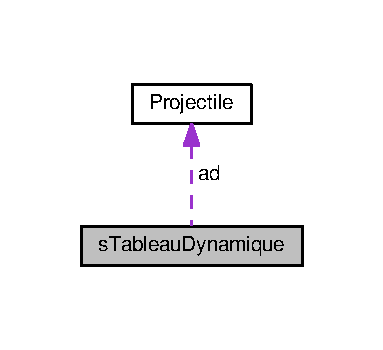
\includegraphics[width=184pt]{structs_tableau_dynamique__coll__graph}
\end{center}
\end{figure}
\subsection*{Data Fields}
\begin{DoxyCompactItemize}
\item 
unsigned int \hyperlink{structs_tableau_dynamique_ac3e3c7196292bbc416a904d29ee638c8}{capacite}
\item 
unsigned int \hyperlink{structs_tableau_dynamique_aaf681889cbd00b7c45951f63b10f969a}{taille\-\_\-utilisee}
\item 
\hyperlink{_jeu_8h_a19f385bd48e6eaff3c61e8abf073263e}{Element\-T\-D} $\ast$ \hyperlink{structs_tableau_dynamique_a3b30ad6492b460f0995b66b2c8889426}{ad}
\end{DoxyCompactItemize}


\subsection{Detailed Description}


Definition at line 13 of file Jeu.\-h.



\subsection{Field Documentation}
\hypertarget{structs_tableau_dynamique_a3b30ad6492b460f0995b66b2c8889426}{\index{s\-Tableau\-Dynamique@{s\-Tableau\-Dynamique}!ad@{ad}}
\index{ad@{ad}!sTableauDynamique@{s\-Tableau\-Dynamique}}
\subsubsection[{ad}]{\setlength{\rightskip}{0pt plus 5cm}{\bf Element\-T\-D}$\ast$ ad}}\label{structs_tableau_dynamique_a3b30ad6492b460f0995b66b2c8889426}


Definition at line 17 of file Jeu.\-h.

\hypertarget{structs_tableau_dynamique_ac3e3c7196292bbc416a904d29ee638c8}{\index{s\-Tableau\-Dynamique@{s\-Tableau\-Dynamique}!capacite@{capacite}}
\index{capacite@{capacite}!sTableauDynamique@{s\-Tableau\-Dynamique}}
\subsubsection[{capacite}]{\setlength{\rightskip}{0pt plus 5cm}unsigned int capacite}}\label{structs_tableau_dynamique_ac3e3c7196292bbc416a904d29ee638c8}


Definition at line 15 of file Jeu.\-h.

\hypertarget{structs_tableau_dynamique_aaf681889cbd00b7c45951f63b10f969a}{\index{s\-Tableau\-Dynamique@{s\-Tableau\-Dynamique}!taille\-\_\-utilisee@{taille\-\_\-utilisee}}
\index{taille\-\_\-utilisee@{taille\-\_\-utilisee}!sTableauDynamique@{s\-Tableau\-Dynamique}}
\subsubsection[{taille\-\_\-utilisee}]{\setlength{\rightskip}{0pt plus 5cm}unsigned int taille\-\_\-utilisee}}\label{structs_tableau_dynamique_aaf681889cbd00b7c45951f63b10f969a}


Definition at line 16 of file Jeu.\-h.



The documentation for this struct was generated from the following file\-:\begin{DoxyCompactItemize}
\item 
/home/enzo/projet\-\_\-fluide/src/\hyperlink{_jeu_8h}{Jeu.\-h}\end{DoxyCompactItemize}

\hypertarget{struct_terrain}{\section{Terrain Struct Reference}
\label{struct_terrain}\index{Terrain@{Terrain}}
}


{\ttfamily \#include $<$Terrain.\-h$>$}



Collaboration diagram for Terrain\-:\nopagebreak
\begin{figure}[H]
\begin{center}
\leavevmode
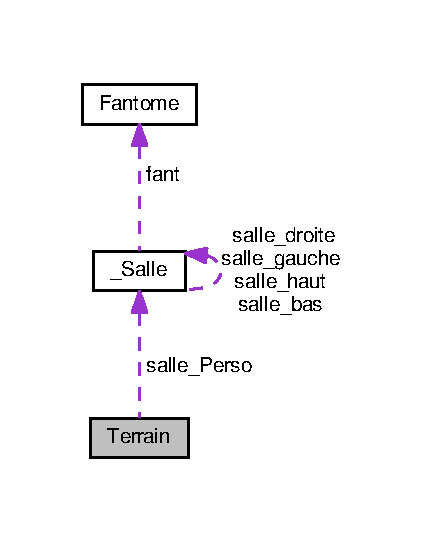
\includegraphics[width=205pt]{struct_terrain__coll__graph}
\end{center}
\end{figure}
\subsection*{Data Fields}
\begin{DoxyCompactItemize}
\item 
int \hyperlink{struct_terrain_a8b0f6ae031a507c3ffb7bf0eec290d46}{dimx}
\item 
int \hyperlink{struct_terrain_a3a072d6ef9c51d085b44eac70f2edff6}{dimy}
\item 
char $\ast$$\ast$ \hyperlink{struct_terrain_a095ef5f32e2dd3c36f801fc514372ee3}{tab}
\item 
\hyperlink{_terrain_8h_a00ea6820934a8f863026cfbfad337db8}{Salle} $\ast$ \hyperlink{struct_terrain_ad00556a521b6c4ae8221f3c9e361cc03}{salle\-\_\-\-Perso}
\end{DoxyCompactItemize}


\subsection{Detailed Description}


Definition at line 37 of file Terrain.\-h.



\subsection{Field Documentation}
\hypertarget{struct_terrain_a8b0f6ae031a507c3ffb7bf0eec290d46}{\index{Terrain@{Terrain}!dimx@{dimx}}
\index{dimx@{dimx}!Terrain@{Terrain}}
\subsubsection[{dimx}]{\setlength{\rightskip}{0pt plus 5cm}int dimx}}\label{struct_terrain_a8b0f6ae031a507c3ffb7bf0eec290d46}


Definition at line 39 of file Terrain.\-h.

\hypertarget{struct_terrain_a3a072d6ef9c51d085b44eac70f2edff6}{\index{Terrain@{Terrain}!dimy@{dimy}}
\index{dimy@{dimy}!Terrain@{Terrain}}
\subsubsection[{dimy}]{\setlength{\rightskip}{0pt plus 5cm}int dimy}}\label{struct_terrain_a3a072d6ef9c51d085b44eac70f2edff6}


Definition at line 40 of file Terrain.\-h.

\hypertarget{struct_terrain_ad00556a521b6c4ae8221f3c9e361cc03}{\index{Terrain@{Terrain}!salle\-\_\-\-Perso@{salle\-\_\-\-Perso}}
\index{salle\-\_\-\-Perso@{salle\-\_\-\-Perso}!Terrain@{Terrain}}
\subsubsection[{salle\-\_\-\-Perso}]{\setlength{\rightskip}{0pt plus 5cm}{\bf Salle}$\ast$ salle\-\_\-\-Perso}}\label{struct_terrain_ad00556a521b6c4ae8221f3c9e361cc03}


Definition at line 42 of file Terrain.\-h.

\hypertarget{struct_terrain_a095ef5f32e2dd3c36f801fc514372ee3}{\index{Terrain@{Terrain}!tab@{tab}}
\index{tab@{tab}!Terrain@{Terrain}}
\subsubsection[{tab}]{\setlength{\rightskip}{0pt plus 5cm}char$\ast$$\ast$ tab}}\label{struct_terrain_a095ef5f32e2dd3c36f801fc514372ee3}


Definition at line 41 of file Terrain.\-h.



The documentation for this struct was generated from the following file\-:\begin{DoxyCompactItemize}
\item 
/home/enzo/projet\-\_\-fluide/src/\hyperlink{_terrain_8h}{Terrain.\-h}\end{DoxyCompactItemize}

\chapter{File Documentation}
\hypertarget{_fromage_8c}{\section{/home/enzo/projet\-\_\-fluide/src/\-Fromage.c File Reference}
\label{_fromage_8c}\index{/home/enzo/projet\-\_\-fluide/src/\-Fromage.\-c@{/home/enzo/projet\-\_\-fluide/src/\-Fromage.\-c}}
}
{\ttfamily \#include \char`\"{}Fromage.\-h\char`\"{}}\\*
{\ttfamily \#include \char`\"{}sdl\-Jeu.\-h\char`\"{}}\\*
Include dependency graph for Fromage.\-c\-:\nopagebreak
\begin{figure}[H]
\begin{center}
\leavevmode
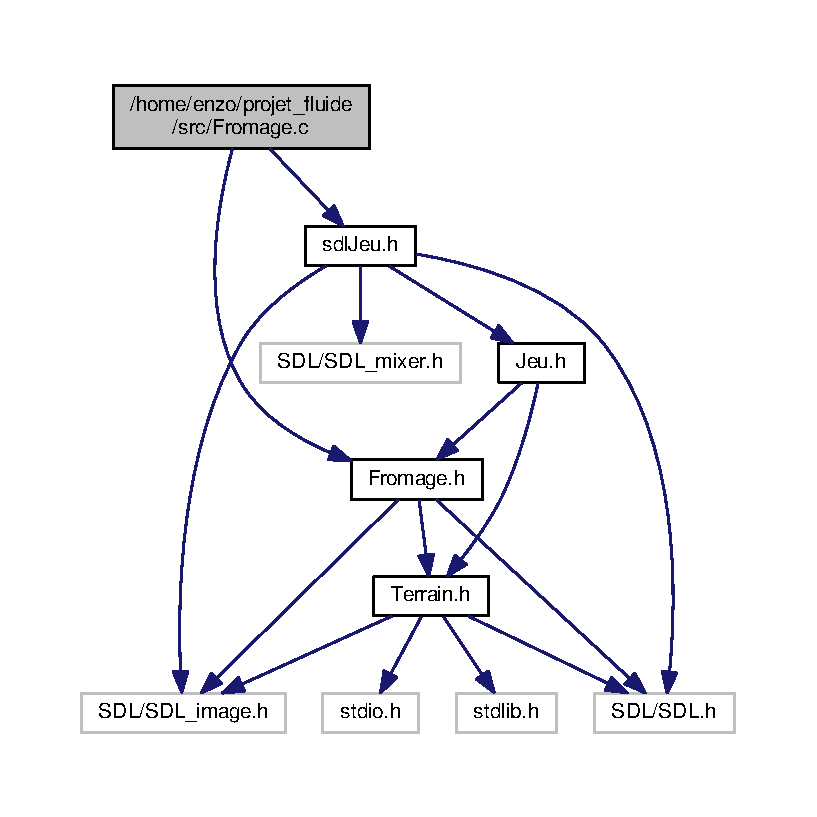
\includegraphics[width=350pt]{_fromage_8c__incl}
\end{center}
\end{figure}
\subsection*{Macros}
\begin{DoxyCompactItemize}
\item 
\#define \hyperlink{_fromage_8c_acd0f9b88c35112b35f67d3cde4b2365c}{H\-A\-U\-T}~0
\item 
\#define \hyperlink{_fromage_8c_af625d3f3bc022848a558f2b18def5b15}{D\-R\-O\-I\-T\-E}~p\-From-\/$>$vitesse
\item 
\#define \hyperlink{_fromage_8c_abd7bcdd3b14eec4414469f88f2bd8f12}{B\-A\-S}~2
\item 
\#define \hyperlink{_fromage_8c_af07f8bf974fdf76afd17f2b97ac15a22}{G\-A\-U\-C\-H\-E}~3
\item 
\#define \hyperlink{_fromage_8c_a7dcae438e7824a23ed30d2139c1eff89}{A\-U\-C\-U\-N\-E\-\_\-\-D\-I\-R\-E\-C\-T\-I\-O\-N}~4
\item 
\#define \hyperlink{_fromage_8c_a4104d8bac5f71c40e72de6aa5080e853}{D\-I\-R\-E\-C\-T\-I\-O\-N\-\_\-\-H\-A\-U\-T}~5
\item 
\#define \hyperlink{_fromage_8c_a17b219a9666ba50f527efe5fecf9de4c}{D\-I\-R\-E\-C\-T\-I\-O\-N\-\_\-\-D\-R\-O\-I\-T\-E}~6
\item 
\#define \hyperlink{_fromage_8c_a0439327d50e1021a81cff4d7dce7ac12}{D\-I\-R\-E\-C\-T\-I\-O\-N\-\_\-\-B\-A\-S}~7
\item 
\#define \hyperlink{_fromage_8c_aab6eb63c11e2bab5f85e8488a3b30d5d}{D\-I\-R\-E\-C\-T\-I\-O\-N\-\_\-\-G\-A\-U\-C\-H\-E}~8
\end{DoxyCompactItemize}
\subsection*{Functions}
\begin{DoxyCompactItemize}
\item 
void \hyperlink{_fromage_8c_a0ab0915ae62ade36bec9bba192c34614}{from\-Init} (\hyperlink{struct_fromage}{Fromage} $\ast$p\-From)
\begin{DoxyCompactList}\small\item\em Initialise les coordonnées de bases et autres variable de notre personnage. \end{DoxyCompactList}\item 
void \hyperlink{_fromage_8c_a365ad04b0043379b598c870904130f83}{from\-Diag\-G\-B} (\hyperlink{struct_fromage}{Fromage} $\ast$p\-From, const \hyperlink{struct_terrain}{Terrain} $\ast$p\-Ter)
\item 
void \hyperlink{_fromage_8c_afe3587533c99fc07fa05e4bd3b698e2d}{from\-Diag\-G\-H} (\hyperlink{struct_fromage}{Fromage} $\ast$p\-From, const \hyperlink{struct_terrain}{Terrain} $\ast$p\-Ter)
\item 
void \hyperlink{_fromage_8c_a415d063435745d17fffbd85768a98745}{from\-Diag\-D\-B} (\hyperlink{struct_fromage}{Fromage} $\ast$p\-From, const \hyperlink{struct_terrain}{Terrain} $\ast$p\-Ter)
\item 
void \hyperlink{_fromage_8c_a0421477017fd29fa3ec280a5ad3b8636}{from\-Diag\-D\-H} (\hyperlink{struct_fromage}{Fromage} $\ast$p\-From, const \hyperlink{struct_terrain}{Terrain} $\ast$p\-Ter)
\item 
void \hyperlink{_fromage_8c_a1b01ae253751f07cae61840adada464c}{from\-Gauche} (\hyperlink{struct_fromage}{Fromage} $\ast$p\-From, const \hyperlink{struct_terrain}{Terrain} $\ast$p\-Ter)
\begin{DoxyCompactList}\small\item\em le personnage vas vers la gauche \end{DoxyCompactList}\item 
void \hyperlink{_fromage_8c_a7a9d7a9f21a8a8416994073ea5b5d0db}{from\-Droite} (\hyperlink{struct_fromage}{Fromage} $\ast$p\-From, const \hyperlink{struct_terrain}{Terrain} $\ast$p\-Ter)
\begin{DoxyCompactList}\small\item\em le personnage vas vers la droite \end{DoxyCompactList}\item 
void \hyperlink{_fromage_8c_a5863a40a7e9e51a065af35d0efeeb7ee}{from\-Haut} (\hyperlink{struct_fromage}{Fromage} $\ast$p\-From, const \hyperlink{struct_terrain}{Terrain} $\ast$p\-Ter)
\item 
void \hyperlink{_fromage_8c_a7b6cb1da5e864487c3802d7698929165}{from\-Chute} (\hyperlink{struct_fromage}{Fromage} $\ast$p\-From, const \hyperlink{struct_terrain}{Terrain} $\ast$p\-Ter)
\item 
void \hyperlink{_fromage_8c_a6b65f6ef20e9b627bf6c3ce5044bcb3a}{from\-Bas} (\hyperlink{struct_fromage}{Fromage} $\ast$p\-From, const \hyperlink{struct_terrain}{Terrain} $\ast$p\-Ter)
\begin{DoxyCompactList}\small\item\em le personnage vas vers le bas \end{DoxyCompactList}\item 
int \hyperlink{_fromage_8c_a4577e7688f86fb847a8990b0b6ceaf68}{from\-Get\-X} (const \hyperlink{struct_fromage}{Fromage} $\ast$p\-From)
\begin{DoxyCompactList}\small\item\em donne la position en x du perso \end{DoxyCompactList}\item 
int \hyperlink{_fromage_8c_ab4d8527e7702c9b9a6828d4305581894}{from\-Get\-Y} (const \hyperlink{struct_fromage}{Fromage} $\ast$p\-From)
\begin{DoxyCompactList}\small\item\em donne la position en y du perso \end{DoxyCompactList}\item 
int \hyperlink{_fromage_8c_ada12e1da3385503d6dfb4f2861dd5049}{from\-Gethp} (const \hyperlink{struct_fromage}{Fromage} $\ast$p\-From)
\begin{DoxyCompactList}\small\item\em donne les point de vie du perso \end{DoxyCompactList}\item 
void \hyperlink{_fromage_8c_a744f5a56a52afbd86c3318bd16ce63d4}{from\-Sethp} (int x, \hyperlink{struct_fromage}{Fromage} $\ast$p\-From)
\begin{DoxyCompactList}\small\item\em change les point de vie du perso \end{DoxyCompactList}\end{DoxyCompactItemize}


\subsection{Macro Definition Documentation}
\hypertarget{_fromage_8c_a7dcae438e7824a23ed30d2139c1eff89}{\index{Fromage.\-c@{Fromage.\-c}!A\-U\-C\-U\-N\-E\-\_\-\-D\-I\-R\-E\-C\-T\-I\-O\-N@{A\-U\-C\-U\-N\-E\-\_\-\-D\-I\-R\-E\-C\-T\-I\-O\-N}}
\index{A\-U\-C\-U\-N\-E\-\_\-\-D\-I\-R\-E\-C\-T\-I\-O\-N@{A\-U\-C\-U\-N\-E\-\_\-\-D\-I\-R\-E\-C\-T\-I\-O\-N}!Fromage.c@{Fromage.\-c}}
\subsubsection[{A\-U\-C\-U\-N\-E\-\_\-\-D\-I\-R\-E\-C\-T\-I\-O\-N}]{\setlength{\rightskip}{0pt plus 5cm}\#define A\-U\-C\-U\-N\-E\-\_\-\-D\-I\-R\-E\-C\-T\-I\-O\-N~4}}\label{_fromage_8c_a7dcae438e7824a23ed30d2139c1eff89}


Definition at line 8 of file Fromage.\-c.

\hypertarget{_fromage_8c_abd7bcdd3b14eec4414469f88f2bd8f12}{\index{Fromage.\-c@{Fromage.\-c}!B\-A\-S@{B\-A\-S}}
\index{B\-A\-S@{B\-A\-S}!Fromage.c@{Fromage.\-c}}
\subsubsection[{B\-A\-S}]{\setlength{\rightskip}{0pt plus 5cm}\#define B\-A\-S~2}}\label{_fromage_8c_abd7bcdd3b14eec4414469f88f2bd8f12}


Definition at line 5 of file Fromage.\-c.

\hypertarget{_fromage_8c_a0439327d50e1021a81cff4d7dce7ac12}{\index{Fromage.\-c@{Fromage.\-c}!D\-I\-R\-E\-C\-T\-I\-O\-N\-\_\-\-B\-A\-S@{D\-I\-R\-E\-C\-T\-I\-O\-N\-\_\-\-B\-A\-S}}
\index{D\-I\-R\-E\-C\-T\-I\-O\-N\-\_\-\-B\-A\-S@{D\-I\-R\-E\-C\-T\-I\-O\-N\-\_\-\-B\-A\-S}!Fromage.c@{Fromage.\-c}}
\subsubsection[{D\-I\-R\-E\-C\-T\-I\-O\-N\-\_\-\-B\-A\-S}]{\setlength{\rightskip}{0pt plus 5cm}\#define D\-I\-R\-E\-C\-T\-I\-O\-N\-\_\-\-B\-A\-S~7}}\label{_fromage_8c_a0439327d50e1021a81cff4d7dce7ac12}


Definition at line 11 of file Fromage.\-c.

\hypertarget{_fromage_8c_a17b219a9666ba50f527efe5fecf9de4c}{\index{Fromage.\-c@{Fromage.\-c}!D\-I\-R\-E\-C\-T\-I\-O\-N\-\_\-\-D\-R\-O\-I\-T\-E@{D\-I\-R\-E\-C\-T\-I\-O\-N\-\_\-\-D\-R\-O\-I\-T\-E}}
\index{D\-I\-R\-E\-C\-T\-I\-O\-N\-\_\-\-D\-R\-O\-I\-T\-E@{D\-I\-R\-E\-C\-T\-I\-O\-N\-\_\-\-D\-R\-O\-I\-T\-E}!Fromage.c@{Fromage.\-c}}
\subsubsection[{D\-I\-R\-E\-C\-T\-I\-O\-N\-\_\-\-D\-R\-O\-I\-T\-E}]{\setlength{\rightskip}{0pt plus 5cm}\#define D\-I\-R\-E\-C\-T\-I\-O\-N\-\_\-\-D\-R\-O\-I\-T\-E~6}}\label{_fromage_8c_a17b219a9666ba50f527efe5fecf9de4c}


Definition at line 10 of file Fromage.\-c.

\hypertarget{_fromage_8c_aab6eb63c11e2bab5f85e8488a3b30d5d}{\index{Fromage.\-c@{Fromage.\-c}!D\-I\-R\-E\-C\-T\-I\-O\-N\-\_\-\-G\-A\-U\-C\-H\-E@{D\-I\-R\-E\-C\-T\-I\-O\-N\-\_\-\-G\-A\-U\-C\-H\-E}}
\index{D\-I\-R\-E\-C\-T\-I\-O\-N\-\_\-\-G\-A\-U\-C\-H\-E@{D\-I\-R\-E\-C\-T\-I\-O\-N\-\_\-\-G\-A\-U\-C\-H\-E}!Fromage.c@{Fromage.\-c}}
\subsubsection[{D\-I\-R\-E\-C\-T\-I\-O\-N\-\_\-\-G\-A\-U\-C\-H\-E}]{\setlength{\rightskip}{0pt plus 5cm}\#define D\-I\-R\-E\-C\-T\-I\-O\-N\-\_\-\-G\-A\-U\-C\-H\-E~8}}\label{_fromage_8c_aab6eb63c11e2bab5f85e8488a3b30d5d}


Definition at line 12 of file Fromage.\-c.

\hypertarget{_fromage_8c_a4104d8bac5f71c40e72de6aa5080e853}{\index{Fromage.\-c@{Fromage.\-c}!D\-I\-R\-E\-C\-T\-I\-O\-N\-\_\-\-H\-A\-U\-T@{D\-I\-R\-E\-C\-T\-I\-O\-N\-\_\-\-H\-A\-U\-T}}
\index{D\-I\-R\-E\-C\-T\-I\-O\-N\-\_\-\-H\-A\-U\-T@{D\-I\-R\-E\-C\-T\-I\-O\-N\-\_\-\-H\-A\-U\-T}!Fromage.c@{Fromage.\-c}}
\subsubsection[{D\-I\-R\-E\-C\-T\-I\-O\-N\-\_\-\-H\-A\-U\-T}]{\setlength{\rightskip}{0pt plus 5cm}\#define D\-I\-R\-E\-C\-T\-I\-O\-N\-\_\-\-H\-A\-U\-T~5}}\label{_fromage_8c_a4104d8bac5f71c40e72de6aa5080e853}


Definition at line 9 of file Fromage.\-c.

\hypertarget{_fromage_8c_af625d3f3bc022848a558f2b18def5b15}{\index{Fromage.\-c@{Fromage.\-c}!D\-R\-O\-I\-T\-E@{D\-R\-O\-I\-T\-E}}
\index{D\-R\-O\-I\-T\-E@{D\-R\-O\-I\-T\-E}!Fromage.c@{Fromage.\-c}}
\subsubsection[{D\-R\-O\-I\-T\-E}]{\setlength{\rightskip}{0pt plus 5cm}\#define D\-R\-O\-I\-T\-E~p\-From-\/$>$vitesse}}\label{_fromage_8c_af625d3f3bc022848a558f2b18def5b15}


Definition at line 4 of file Fromage.\-c.

\hypertarget{_fromage_8c_af07f8bf974fdf76afd17f2b97ac15a22}{\index{Fromage.\-c@{Fromage.\-c}!G\-A\-U\-C\-H\-E@{G\-A\-U\-C\-H\-E}}
\index{G\-A\-U\-C\-H\-E@{G\-A\-U\-C\-H\-E}!Fromage.c@{Fromage.\-c}}
\subsubsection[{G\-A\-U\-C\-H\-E}]{\setlength{\rightskip}{0pt plus 5cm}\#define G\-A\-U\-C\-H\-E~3}}\label{_fromage_8c_af07f8bf974fdf76afd17f2b97ac15a22}


Definition at line 6 of file Fromage.\-c.

\hypertarget{_fromage_8c_acd0f9b88c35112b35f67d3cde4b2365c}{\index{Fromage.\-c@{Fromage.\-c}!H\-A\-U\-T@{H\-A\-U\-T}}
\index{H\-A\-U\-T@{H\-A\-U\-T}!Fromage.c@{Fromage.\-c}}
\subsubsection[{H\-A\-U\-T}]{\setlength{\rightskip}{0pt plus 5cm}\#define H\-A\-U\-T~0}}\label{_fromage_8c_acd0f9b88c35112b35f67d3cde4b2365c}


Definition at line 3 of file Fromage.\-c.



\subsection{Function Documentation}
\hypertarget{_fromage_8c_a6b65f6ef20e9b627bf6c3ce5044bcb3a}{\index{Fromage.\-c@{Fromage.\-c}!from\-Bas@{from\-Bas}}
\index{from\-Bas@{from\-Bas}!Fromage.c@{Fromage.\-c}}
\subsubsection[{from\-Bas}]{\setlength{\rightskip}{0pt plus 5cm}void from\-Bas (
\begin{DoxyParamCaption}
\item[{{\bf Fromage} $\ast$}]{, }
\item[{const {\bf Terrain} $\ast$}]{}
\end{DoxyParamCaption}
)}}\label{_fromage_8c_a6b65f6ef20e9b627bf6c3ce5044bcb3a}


le personnage vas vers le bas 


\begin{DoxyParams}{Parameters}
{\em \hyperlink{struct_fromage}{Fromage}} & $\ast$ \\
\hline
{\em const} & \hyperlink{struct_terrain}{Terrain} $\ast$ \\
\hline
\end{DoxyParams}


Definition at line 106 of file Fromage.\-c.



Here is the call graph for this function\-:\nopagebreak
\begin{figure}[H]
\begin{center}
\leavevmode
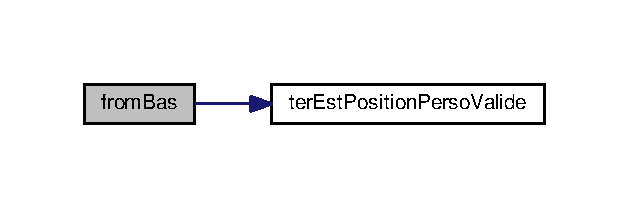
\includegraphics[width=302pt]{_fromage_8c_a6b65f6ef20e9b627bf6c3ce5044bcb3a_cgraph}
\end{center}
\end{figure}


\hypertarget{_fromage_8c_a7b6cb1da5e864487c3802d7698929165}{\index{Fromage.\-c@{Fromage.\-c}!from\-Chute@{from\-Chute}}
\index{from\-Chute@{from\-Chute}!Fromage.c@{Fromage.\-c}}
\subsubsection[{from\-Chute}]{\setlength{\rightskip}{0pt plus 5cm}void from\-Chute (
\begin{DoxyParamCaption}
\item[{{\bf Fromage} $\ast$}]{p\-From, }
\item[{const {\bf Terrain} $\ast$}]{p\-Ter}
\end{DoxyParamCaption}
)}}\label{_fromage_8c_a7b6cb1da5e864487c3802d7698929165}


Definition at line 99 of file Fromage.\-c.

\hypertarget{_fromage_8c_a415d063435745d17fffbd85768a98745}{\index{Fromage.\-c@{Fromage.\-c}!from\-Diag\-D\-B@{from\-Diag\-D\-B}}
\index{from\-Diag\-D\-B@{from\-Diag\-D\-B}!Fromage.c@{Fromage.\-c}}
\subsubsection[{from\-Diag\-D\-B}]{\setlength{\rightskip}{0pt plus 5cm}void from\-Diag\-D\-B (
\begin{DoxyParamCaption}
\item[{{\bf Fromage} $\ast$}]{p\-From, }
\item[{const {\bf Terrain} $\ast$}]{p\-Ter}
\end{DoxyParamCaption}
)}}\label{_fromage_8c_a415d063435745d17fffbd85768a98745}


Definition at line 54 of file Fromage.\-c.



Here is the call graph for this function\-:\nopagebreak
\begin{figure}[H]
\begin{center}
\leavevmode
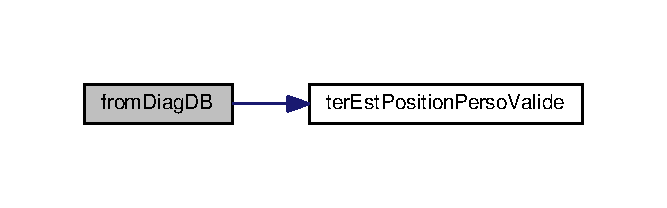
\includegraphics[width=320pt]{_fromage_8c_a415d063435745d17fffbd85768a98745_cgraph}
\end{center}
\end{figure}


\hypertarget{_fromage_8c_a0421477017fd29fa3ec280a5ad3b8636}{\index{Fromage.\-c@{Fromage.\-c}!from\-Diag\-D\-H@{from\-Diag\-D\-H}}
\index{from\-Diag\-D\-H@{from\-Diag\-D\-H}!Fromage.c@{Fromage.\-c}}
\subsubsection[{from\-Diag\-D\-H}]{\setlength{\rightskip}{0pt plus 5cm}void from\-Diag\-D\-H (
\begin{DoxyParamCaption}
\item[{{\bf Fromage} $\ast$}]{p\-From, }
\item[{const {\bf Terrain} $\ast$}]{p\-Ter}
\end{DoxyParamCaption}
)}}\label{_fromage_8c_a0421477017fd29fa3ec280a5ad3b8636}


Definition at line 63 of file Fromage.\-c.



Here is the call graph for this function\-:\nopagebreak
\begin{figure}[H]
\begin{center}
\leavevmode
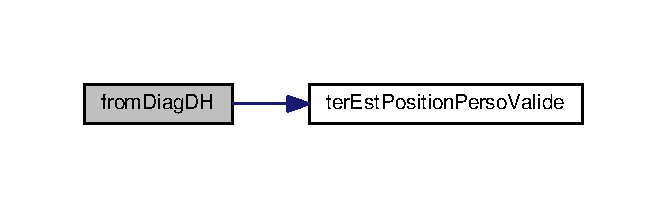
\includegraphics[width=320pt]{_fromage_8c_a0421477017fd29fa3ec280a5ad3b8636_cgraph}
\end{center}
\end{figure}


\hypertarget{_fromage_8c_a365ad04b0043379b598c870904130f83}{\index{Fromage.\-c@{Fromage.\-c}!from\-Diag\-G\-B@{from\-Diag\-G\-B}}
\index{from\-Diag\-G\-B@{from\-Diag\-G\-B}!Fromage.c@{Fromage.\-c}}
\subsubsection[{from\-Diag\-G\-B}]{\setlength{\rightskip}{0pt plus 5cm}void from\-Diag\-G\-B (
\begin{DoxyParamCaption}
\item[{{\bf Fromage} $\ast$}]{p\-From, }
\item[{const {\bf Terrain} $\ast$}]{p\-Ter}
\end{DoxyParamCaption}
)}}\label{_fromage_8c_a365ad04b0043379b598c870904130f83}


Definition at line 36 of file Fromage.\-c.



Here is the call graph for this function\-:\nopagebreak
\begin{figure}[H]
\begin{center}
\leavevmode
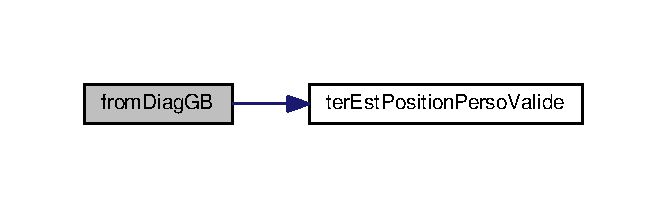
\includegraphics[width=320pt]{_fromage_8c_a365ad04b0043379b598c870904130f83_cgraph}
\end{center}
\end{figure}


\hypertarget{_fromage_8c_afe3587533c99fc07fa05e4bd3b698e2d}{\index{Fromage.\-c@{Fromage.\-c}!from\-Diag\-G\-H@{from\-Diag\-G\-H}}
\index{from\-Diag\-G\-H@{from\-Diag\-G\-H}!Fromage.c@{Fromage.\-c}}
\subsubsection[{from\-Diag\-G\-H}]{\setlength{\rightskip}{0pt plus 5cm}void from\-Diag\-G\-H (
\begin{DoxyParamCaption}
\item[{{\bf Fromage} $\ast$}]{p\-From, }
\item[{const {\bf Terrain} $\ast$}]{p\-Ter}
\end{DoxyParamCaption}
)}}\label{_fromage_8c_afe3587533c99fc07fa05e4bd3b698e2d}


Definition at line 45 of file Fromage.\-c.



Here is the call graph for this function\-:\nopagebreak
\begin{figure}[H]
\begin{center}
\leavevmode
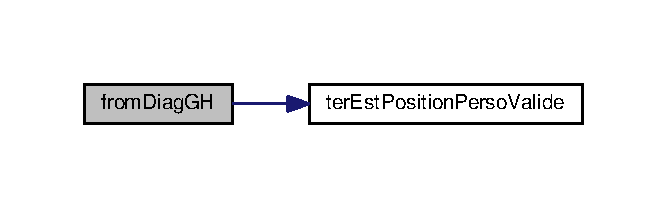
\includegraphics[width=320pt]{_fromage_8c_afe3587533c99fc07fa05e4bd3b698e2d_cgraph}
\end{center}
\end{figure}


\hypertarget{_fromage_8c_a7a9d7a9f21a8a8416994073ea5b5d0db}{\index{Fromage.\-c@{Fromage.\-c}!from\-Droite@{from\-Droite}}
\index{from\-Droite@{from\-Droite}!Fromage.c@{Fromage.\-c}}
\subsubsection[{from\-Droite}]{\setlength{\rightskip}{0pt plus 5cm}void from\-Droite (
\begin{DoxyParamCaption}
\item[{{\bf Fromage} $\ast$}]{, }
\item[{const {\bf Terrain} $\ast$}]{}
\end{DoxyParamCaption}
)}}\label{_fromage_8c_a7a9d7a9f21a8a8416994073ea5b5d0db}


le personnage vas vers la droite 


\begin{DoxyParams}{Parameters}
{\em \hyperlink{struct_fromage}{Fromage}} & $\ast$ \\
\hline
{\em const} & \hyperlink{struct_terrain}{Terrain} $\ast$ \\
\hline
\end{DoxyParams}


Definition at line 81 of file Fromage.\-c.



Here is the call graph for this function\-:\nopagebreak
\begin{figure}[H]
\begin{center}
\leavevmode
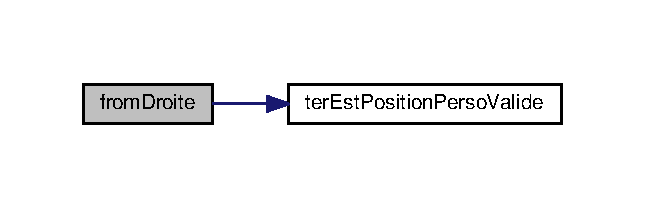
\includegraphics[width=310pt]{_fromage_8c_a7a9d7a9f21a8a8416994073ea5b5d0db_cgraph}
\end{center}
\end{figure}


\hypertarget{_fromage_8c_a1b01ae253751f07cae61840adada464c}{\index{Fromage.\-c@{Fromage.\-c}!from\-Gauche@{from\-Gauche}}
\index{from\-Gauche@{from\-Gauche}!Fromage.c@{Fromage.\-c}}
\subsubsection[{from\-Gauche}]{\setlength{\rightskip}{0pt plus 5cm}void from\-Gauche (
\begin{DoxyParamCaption}
\item[{{\bf Fromage} $\ast$}]{, }
\item[{const {\bf Terrain} $\ast$}]{}
\end{DoxyParamCaption}
)}}\label{_fromage_8c_a1b01ae253751f07cae61840adada464c}


le personnage vas vers la gauche 


\begin{DoxyParams}{Parameters}
{\em \hyperlink{struct_fromage}{Fromage}} & $\ast$ \\
\hline
{\em const} & \hyperlink{struct_terrain}{Terrain} $\ast$ \\
\hline
\end{DoxyParams}


Definition at line 72 of file Fromage.\-c.



Here is the call graph for this function\-:\nopagebreak
\begin{figure}[H]
\begin{center}
\leavevmode
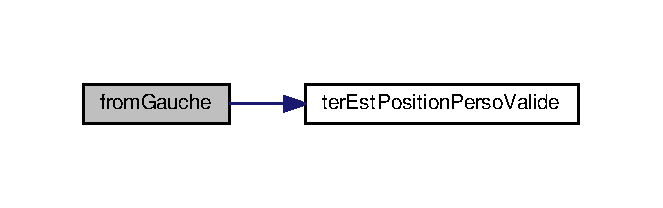
\includegraphics[width=318pt]{_fromage_8c_a1b01ae253751f07cae61840adada464c_cgraph}
\end{center}
\end{figure}


\hypertarget{_fromage_8c_ada12e1da3385503d6dfb4f2861dd5049}{\index{Fromage.\-c@{Fromage.\-c}!from\-Gethp@{from\-Gethp}}
\index{from\-Gethp@{from\-Gethp}!Fromage.c@{Fromage.\-c}}
\subsubsection[{from\-Gethp}]{\setlength{\rightskip}{0pt plus 5cm}int from\-Gethp (
\begin{DoxyParamCaption}
\item[{const {\bf Fromage} $\ast$}]{}
\end{DoxyParamCaption}
)}}\label{_fromage_8c_ada12e1da3385503d6dfb4f2861dd5049}


donne les point de vie du perso 


\begin{DoxyParams}{Parameters}
{\em \hyperlink{struct_fromage}{Fromage}} & $\ast$ \\
\hline
\end{DoxyParams}


Definition at line 123 of file Fromage.\-c.

\hypertarget{_fromage_8c_a4577e7688f86fb847a8990b0b6ceaf68}{\index{Fromage.\-c@{Fromage.\-c}!from\-Get\-X@{from\-Get\-X}}
\index{from\-Get\-X@{from\-Get\-X}!Fromage.c@{Fromage.\-c}}
\subsubsection[{from\-Get\-X}]{\setlength{\rightskip}{0pt plus 5cm}int from\-Get\-X (
\begin{DoxyParamCaption}
\item[{const {\bf Fromage} $\ast$}]{}
\end{DoxyParamCaption}
)}}\label{_fromage_8c_a4577e7688f86fb847a8990b0b6ceaf68}


donne la position en x du perso 


\begin{DoxyParams}{Parameters}
{\em \hyperlink{struct_fromage}{Fromage}} & $\ast$ \\
\hline
\end{DoxyParams}


Definition at line 114 of file Fromage.\-c.

\hypertarget{_fromage_8c_ab4d8527e7702c9b9a6828d4305581894}{\index{Fromage.\-c@{Fromage.\-c}!from\-Get\-Y@{from\-Get\-Y}}
\index{from\-Get\-Y@{from\-Get\-Y}!Fromage.c@{Fromage.\-c}}
\subsubsection[{from\-Get\-Y}]{\setlength{\rightskip}{0pt plus 5cm}int from\-Get\-Y (
\begin{DoxyParamCaption}
\item[{const {\bf Fromage} $\ast$}]{}
\end{DoxyParamCaption}
)}}\label{_fromage_8c_ab4d8527e7702c9b9a6828d4305581894}


donne la position en y du perso 


\begin{DoxyParams}{Parameters}
{\em \hyperlink{struct_fromage}{Fromage}} & $\ast$ \\
\hline
\end{DoxyParams}


Definition at line 119 of file Fromage.\-c.

\hypertarget{_fromage_8c_a5863a40a7e9e51a065af35d0efeeb7ee}{\index{Fromage.\-c@{Fromage.\-c}!from\-Haut@{from\-Haut}}
\index{from\-Haut@{from\-Haut}!Fromage.c@{Fromage.\-c}}
\subsubsection[{from\-Haut}]{\setlength{\rightskip}{0pt plus 5cm}void from\-Haut (
\begin{DoxyParamCaption}
\item[{{\bf Fromage} $\ast$}]{p\-From, }
\item[{const {\bf Terrain} $\ast$}]{p\-Ter}
\end{DoxyParamCaption}
)}}\label{_fromage_8c_a5863a40a7e9e51a065af35d0efeeb7ee}


Definition at line 92 of file Fromage.\-c.



Here is the call graph for this function\-:\nopagebreak
\begin{figure}[H]
\begin{center}
\leavevmode
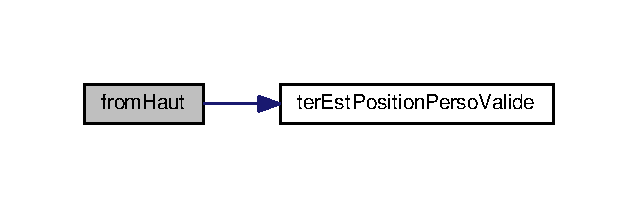
\includegraphics[width=306pt]{_fromage_8c_a5863a40a7e9e51a065af35d0efeeb7ee_cgraph}
\end{center}
\end{figure}


\hypertarget{_fromage_8c_a0ab0915ae62ade36bec9bba192c34614}{\index{Fromage.\-c@{Fromage.\-c}!from\-Init@{from\-Init}}
\index{from\-Init@{from\-Init}!Fromage.c@{Fromage.\-c}}
\subsubsection[{from\-Init}]{\setlength{\rightskip}{0pt plus 5cm}void from\-Init (
\begin{DoxyParamCaption}
\item[{{\bf Fromage} $\ast$}]{}
\end{DoxyParamCaption}
)}}\label{_fromage_8c_a0ab0915ae62ade36bec9bba192c34614}


Initialise les coordonnées de bases et autres variable de notre personnage. 


\begin{DoxyParams}{Parameters}
{\em \hyperlink{struct_fromage}{Fromage}} & $\ast$ \\
\hline
\end{DoxyParams}


Definition at line 13 of file Fromage.\-c.

\hypertarget{_fromage_8c_a744f5a56a52afbd86c3318bd16ce63d4}{\index{Fromage.\-c@{Fromage.\-c}!from\-Sethp@{from\-Sethp}}
\index{from\-Sethp@{from\-Sethp}!Fromage.c@{Fromage.\-c}}
\subsubsection[{from\-Sethp}]{\setlength{\rightskip}{0pt plus 5cm}void from\-Sethp (
\begin{DoxyParamCaption}
\item[{int}]{, }
\item[{{\bf Fromage} $\ast$}]{}
\end{DoxyParamCaption}
)}}\label{_fromage_8c_a744f5a56a52afbd86c3318bd16ce63d4}


change les point de vie du perso 


\begin{DoxyParams}{Parameters}
{\em \hyperlink{struct_fromage}{Fromage}} & $\ast$ \\
\hline
\end{DoxyParams}


Definition at line 127 of file Fromage.\-c.


\hypertarget{_fromage_8h}{\section{/home/enzo/projet\-\_\-fluide/src/\-Fromage.h File Reference}
\label{_fromage_8h}\index{/home/enzo/projet\-\_\-fluide/src/\-Fromage.\-h@{/home/enzo/projet\-\_\-fluide/src/\-Fromage.\-h}}
}
{\ttfamily \#include $<$S\-D\-L/\-S\-D\-L.\-h$>$}\\*
{\ttfamily \#include $<$S\-D\-L/\-S\-D\-L\-\_\-image.\-h$>$}\\*
{\ttfamily \#include \char`\"{}Terrain.\-h\char`\"{}}\\*
Include dependency graph for Fromage.\-h\-:\nopagebreak
\begin{figure}[H]
\begin{center}
\leavevmode
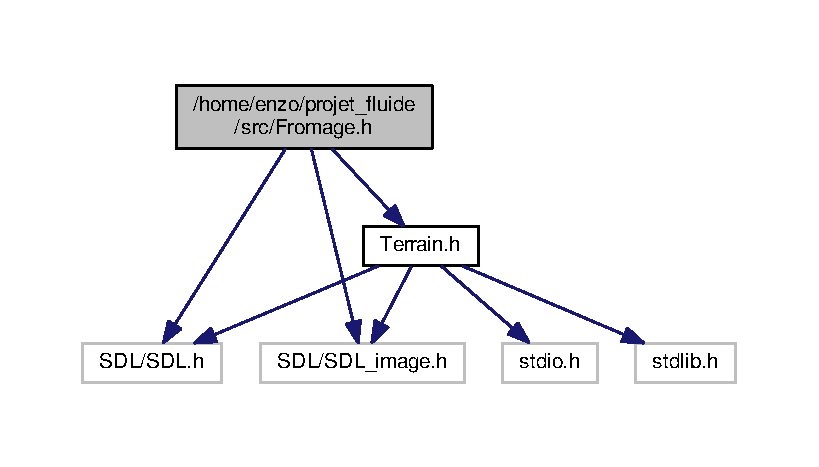
\includegraphics[width=350pt]{_fromage_8h__incl}
\end{center}
\end{figure}
This graph shows which files directly or indirectly include this file\-:
\nopagebreak
\begin{figure}[H]
\begin{center}
\leavevmode
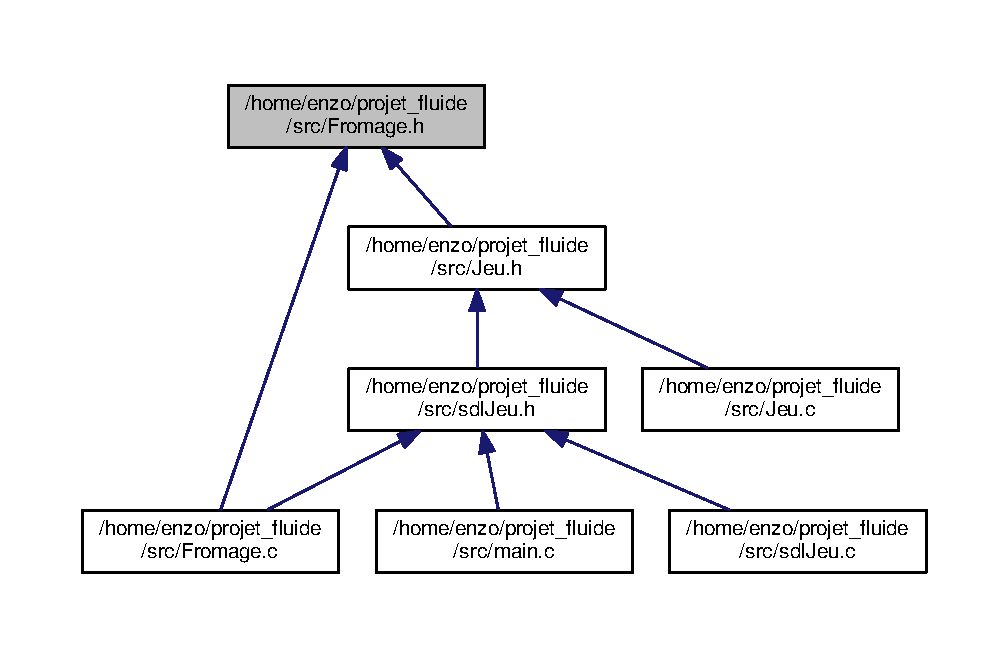
\includegraphics[width=350pt]{_fromage_8h__dep__incl}
\end{center}
\end{figure}
\subsection*{Data Structures}
\begin{DoxyCompactItemize}
\item 
struct \hyperlink{struct_fromage}{Fromage}
\end{DoxyCompactItemize}
\subsection*{Functions}
\begin{DoxyCompactItemize}
\item 
void \hyperlink{_fromage_8h_a3a464aadf40553039f34259b6d29705e}{from\-Init} (\hyperlink{struct_fromage}{Fromage} $\ast$)
\begin{DoxyCompactList}\small\item\em Initialise les coordonnées de bases et autres variable de notre personnage. \end{DoxyCompactList}\item 
void \hyperlink{_fromage_8h_a28417ee81d3c713a73afbdba0473f02a}{from\-Gauche} (\hyperlink{struct_fromage}{Fromage} $\ast$, const \hyperlink{struct_terrain}{Terrain} $\ast$)
\begin{DoxyCompactList}\small\item\em le personnage vas vers la gauche \end{DoxyCompactList}\item 
void \hyperlink{_fromage_8h_a0133c0a17541f03d916e74757482fc15}{from\-Droite} (\hyperlink{struct_fromage}{Fromage} $\ast$, const \hyperlink{struct_terrain}{Terrain} $\ast$)
\begin{DoxyCompactList}\small\item\em le personnage vas vers la droite \end{DoxyCompactList}\item 
void \hyperlink{_fromage_8h_a9d613055bca68909ec3ab656e7365e75}{from\-Bas} (\hyperlink{struct_fromage}{Fromage} $\ast$, const \hyperlink{struct_terrain}{Terrain} $\ast$)
\begin{DoxyCompactList}\small\item\em le personnage vas vers le bas \end{DoxyCompactList}\item 
int \hyperlink{_fromage_8h_a0c17bfd9318ebd9c0a14c552c47b5cda}{from\-Get\-X} (const \hyperlink{struct_fromage}{Fromage} $\ast$)
\begin{DoxyCompactList}\small\item\em donne la position en x du perso \end{DoxyCompactList}\item 
int \hyperlink{_fromage_8h_ad6517a50346a66540015abfb037750ef}{from\-Get\-Y} (const \hyperlink{struct_fromage}{Fromage} $\ast$)
\begin{DoxyCompactList}\small\item\em donne la position en y du perso \end{DoxyCompactList}\item 
int \hyperlink{_fromage_8h_ac3d77de3eb25604ecb152dc234c1b16d}{from\-Gethp} (const \hyperlink{struct_fromage}{Fromage} $\ast$)
\begin{DoxyCompactList}\small\item\em donne les point de vie du perso \end{DoxyCompactList}\item 
void \hyperlink{_fromage_8h_a1fed9a641a1f86497909ac80d35fe785}{from\-Sethp} (int, \hyperlink{struct_fromage}{Fromage} $\ast$)
\begin{DoxyCompactList}\small\item\em change les point de vie du perso \end{DoxyCompactList}\end{DoxyCompactItemize}


\subsection{Function Documentation}
\hypertarget{_fromage_8h_a9d613055bca68909ec3ab656e7365e75}{\index{Fromage.\-h@{Fromage.\-h}!from\-Bas@{from\-Bas}}
\index{from\-Bas@{from\-Bas}!Fromage.h@{Fromage.\-h}}
\subsubsection[{from\-Bas}]{\setlength{\rightskip}{0pt plus 5cm}void from\-Bas (
\begin{DoxyParamCaption}
\item[{{\bf Fromage} $\ast$}]{, }
\item[{const {\bf Terrain} $\ast$}]{}
\end{DoxyParamCaption}
)}}\label{_fromage_8h_a9d613055bca68909ec3ab656e7365e75}


le personnage vas vers le bas 


\begin{DoxyParams}{Parameters}
{\em \hyperlink{struct_fromage}{Fromage}} & $\ast$ \\
\hline
{\em const} & \hyperlink{struct_terrain}{Terrain} $\ast$ \\
\hline
\end{DoxyParams}


Definition at line 106 of file Fromage.\-c.



Here is the call graph for this function\-:\nopagebreak
\begin{figure}[H]
\begin{center}
\leavevmode
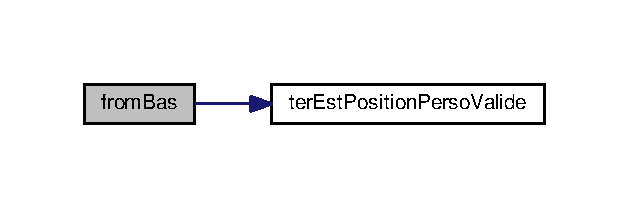
\includegraphics[width=302pt]{_fromage_8h_a9d613055bca68909ec3ab656e7365e75_cgraph}
\end{center}
\end{figure}


\hypertarget{_fromage_8h_a0133c0a17541f03d916e74757482fc15}{\index{Fromage.\-h@{Fromage.\-h}!from\-Droite@{from\-Droite}}
\index{from\-Droite@{from\-Droite}!Fromage.h@{Fromage.\-h}}
\subsubsection[{from\-Droite}]{\setlength{\rightskip}{0pt plus 5cm}void from\-Droite (
\begin{DoxyParamCaption}
\item[{{\bf Fromage} $\ast$}]{, }
\item[{const {\bf Terrain} $\ast$}]{}
\end{DoxyParamCaption}
)}}\label{_fromage_8h_a0133c0a17541f03d916e74757482fc15}


le personnage vas vers la droite 


\begin{DoxyParams}{Parameters}
{\em \hyperlink{struct_fromage}{Fromage}} & $\ast$ \\
\hline
{\em const} & \hyperlink{struct_terrain}{Terrain} $\ast$ \\
\hline
\end{DoxyParams}


Definition at line 81 of file Fromage.\-c.



Here is the call graph for this function\-:\nopagebreak
\begin{figure}[H]
\begin{center}
\leavevmode
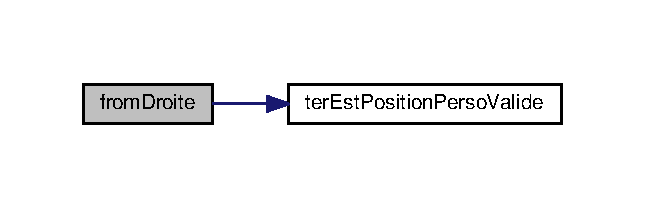
\includegraphics[width=310pt]{_fromage_8h_a0133c0a17541f03d916e74757482fc15_cgraph}
\end{center}
\end{figure}


\hypertarget{_fromage_8h_a28417ee81d3c713a73afbdba0473f02a}{\index{Fromage.\-h@{Fromage.\-h}!from\-Gauche@{from\-Gauche}}
\index{from\-Gauche@{from\-Gauche}!Fromage.h@{Fromage.\-h}}
\subsubsection[{from\-Gauche}]{\setlength{\rightskip}{0pt plus 5cm}void from\-Gauche (
\begin{DoxyParamCaption}
\item[{{\bf Fromage} $\ast$}]{, }
\item[{const {\bf Terrain} $\ast$}]{}
\end{DoxyParamCaption}
)}}\label{_fromage_8h_a28417ee81d3c713a73afbdba0473f02a}


le personnage vas vers la gauche 


\begin{DoxyParams}{Parameters}
{\em \hyperlink{struct_fromage}{Fromage}} & $\ast$ \\
\hline
{\em const} & \hyperlink{struct_terrain}{Terrain} $\ast$ \\
\hline
\end{DoxyParams}


Definition at line 72 of file Fromage.\-c.



Here is the call graph for this function\-:\nopagebreak
\begin{figure}[H]
\begin{center}
\leavevmode
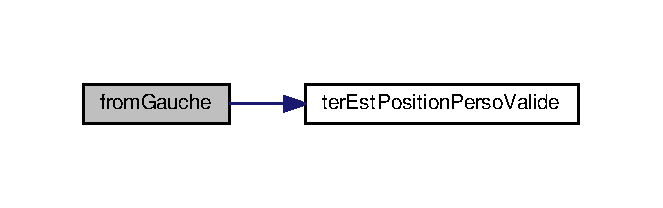
\includegraphics[width=318pt]{_fromage_8h_a28417ee81d3c713a73afbdba0473f02a_cgraph}
\end{center}
\end{figure}


\hypertarget{_fromage_8h_ac3d77de3eb25604ecb152dc234c1b16d}{\index{Fromage.\-h@{Fromage.\-h}!from\-Gethp@{from\-Gethp}}
\index{from\-Gethp@{from\-Gethp}!Fromage.h@{Fromage.\-h}}
\subsubsection[{from\-Gethp}]{\setlength{\rightskip}{0pt plus 5cm}int from\-Gethp (
\begin{DoxyParamCaption}
\item[{const {\bf Fromage} $\ast$}]{}
\end{DoxyParamCaption}
)}}\label{_fromage_8h_ac3d77de3eb25604ecb152dc234c1b16d}


donne les point de vie du perso 


\begin{DoxyParams}{Parameters}
{\em \hyperlink{struct_fromage}{Fromage}} & $\ast$ \\
\hline
\end{DoxyParams}


Definition at line 123 of file Fromage.\-c.

\hypertarget{_fromage_8h_a0c17bfd9318ebd9c0a14c552c47b5cda}{\index{Fromage.\-h@{Fromage.\-h}!from\-Get\-X@{from\-Get\-X}}
\index{from\-Get\-X@{from\-Get\-X}!Fromage.h@{Fromage.\-h}}
\subsubsection[{from\-Get\-X}]{\setlength{\rightskip}{0pt plus 5cm}int from\-Get\-X (
\begin{DoxyParamCaption}
\item[{const {\bf Fromage} $\ast$}]{}
\end{DoxyParamCaption}
)}}\label{_fromage_8h_a0c17bfd9318ebd9c0a14c552c47b5cda}


donne la position en x du perso 


\begin{DoxyParams}{Parameters}
{\em \hyperlink{struct_fromage}{Fromage}} & $\ast$ \\
\hline
\end{DoxyParams}


Definition at line 114 of file Fromage.\-c.

\hypertarget{_fromage_8h_ad6517a50346a66540015abfb037750ef}{\index{Fromage.\-h@{Fromage.\-h}!from\-Get\-Y@{from\-Get\-Y}}
\index{from\-Get\-Y@{from\-Get\-Y}!Fromage.h@{Fromage.\-h}}
\subsubsection[{from\-Get\-Y}]{\setlength{\rightskip}{0pt plus 5cm}int from\-Get\-Y (
\begin{DoxyParamCaption}
\item[{const {\bf Fromage} $\ast$}]{}
\end{DoxyParamCaption}
)}}\label{_fromage_8h_ad6517a50346a66540015abfb037750ef}


donne la position en y du perso 


\begin{DoxyParams}{Parameters}
{\em \hyperlink{struct_fromage}{Fromage}} & $\ast$ \\
\hline
\end{DoxyParams}


Definition at line 119 of file Fromage.\-c.

\hypertarget{_fromage_8h_a3a464aadf40553039f34259b6d29705e}{\index{Fromage.\-h@{Fromage.\-h}!from\-Init@{from\-Init}}
\index{from\-Init@{from\-Init}!Fromage.h@{Fromage.\-h}}
\subsubsection[{from\-Init}]{\setlength{\rightskip}{0pt plus 5cm}void from\-Init (
\begin{DoxyParamCaption}
\item[{{\bf Fromage} $\ast$}]{}
\end{DoxyParamCaption}
)}}\label{_fromage_8h_a3a464aadf40553039f34259b6d29705e}


Initialise les coordonnées de bases et autres variable de notre personnage. 


\begin{DoxyParams}{Parameters}
{\em \hyperlink{struct_fromage}{Fromage}} & $\ast$ \\
\hline
\end{DoxyParams}


Definition at line 13 of file Fromage.\-c.

\hypertarget{_fromage_8h_a1fed9a641a1f86497909ac80d35fe785}{\index{Fromage.\-h@{Fromage.\-h}!from\-Sethp@{from\-Sethp}}
\index{from\-Sethp@{from\-Sethp}!Fromage.h@{Fromage.\-h}}
\subsubsection[{from\-Sethp}]{\setlength{\rightskip}{0pt plus 5cm}void from\-Sethp (
\begin{DoxyParamCaption}
\item[{int}]{, }
\item[{{\bf Fromage} $\ast$}]{}
\end{DoxyParamCaption}
)}}\label{_fromage_8h_a1fed9a641a1f86497909ac80d35fe785}


change les point de vie du perso 


\begin{DoxyParams}{Parameters}
{\em \hyperlink{struct_fromage}{Fromage}} & $\ast$ \\
\hline
\end{DoxyParams}


Definition at line 127 of file Fromage.\-c.


\hypertarget{_jeu_8c}{\section{/home/enzo/projet\-\_\-fluide/src/\-Jeu.c File Reference}
\label{_jeu_8c}\index{/home/enzo/projet\-\_\-fluide/src/\-Jeu.\-c@{/home/enzo/projet\-\_\-fluide/src/\-Jeu.\-c}}
}
{\ttfamily \#include \char`\"{}Jeu.\-h\char`\"{}}\\*
{\ttfamily \#include $<$malloc.\-h$>$}\\*
{\ttfamily \#include $<$stdlib.\-h$>$}\\*
{\ttfamily \#include $<$math.\-h$>$}\\*
Include dependency graph for Jeu.\-c\-:\nopagebreak
\begin{figure}[H]
\begin{center}
\leavevmode
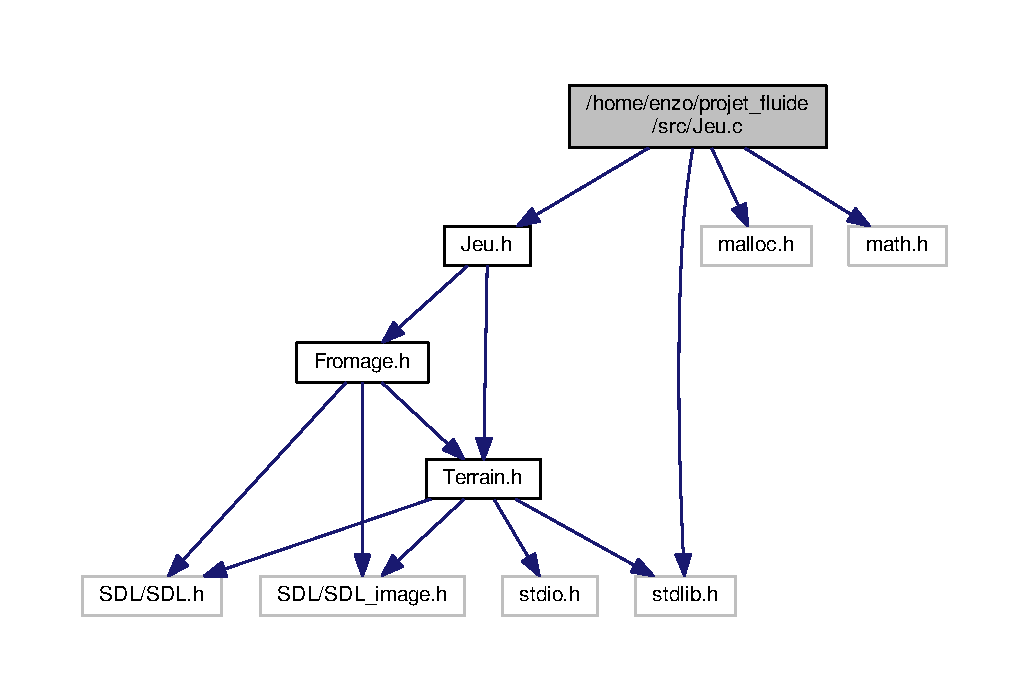
\includegraphics[width=350pt]{_jeu_8c__incl}
\end{center}
\end{figure}
\subsection*{Macros}
\begin{DoxyCompactItemize}
\item 
\#define \hyperlink{_jeu_8c_acd0f9b88c35112b35f67d3cde4b2365c}{H\-A\-U\-T}~0
\item 
\#define \hyperlink{_jeu_8c_af625d3f3bc022848a558f2b18def5b15}{D\-R\-O\-I\-T\-E}~1
\item 
\#define \hyperlink{_jeu_8c_abd7bcdd3b14eec4414469f88f2bd8f12}{B\-A\-S}~2
\item 
\#define \hyperlink{_jeu_8c_af07f8bf974fdf76afd17f2b97ac15a22}{G\-A\-U\-C\-H\-E}~3
\item 
\#define \hyperlink{_jeu_8c_a7dcae438e7824a23ed30d2139c1eff89}{A\-U\-C\-U\-N\-E\-\_\-\-D\-I\-R\-E\-C\-T\-I\-O\-N}~4
\item 
\#define \hyperlink{_jeu_8c_a4104d8bac5f71c40e72de6aa5080e853}{D\-I\-R\-E\-C\-T\-I\-O\-N\-\_\-\-H\-A\-U\-T}~5
\item 
\#define \hyperlink{_jeu_8c_a17b219a9666ba50f527efe5fecf9de4c}{D\-I\-R\-E\-C\-T\-I\-O\-N\-\_\-\-D\-R\-O\-I\-T\-E}~6
\item 
\#define \hyperlink{_jeu_8c_a0439327d50e1021a81cff4d7dce7ac12}{D\-I\-R\-E\-C\-T\-I\-O\-N\-\_\-\-B\-A\-S}~7
\item 
\#define \hyperlink{_jeu_8c_aab6eb63c11e2bab5f85e8488a3b30d5d}{D\-I\-R\-E\-C\-T\-I\-O\-N\-\_\-\-G\-A\-U\-C\-H\-E}~8
\item 
\#define \hyperlink{_jeu_8c_a39bc6ce729110249c344aaff8ff6a0dc}{D\-I\-R\-E\-C\-T\-I\-O\-N\-\_\-\-D\-I\-A\-G\-\_\-\-D\-B}~9
\item 
\#define \hyperlink{_jeu_8c_a76d11649f0994a3577d1a62424a40306}{D\-I\-R\-E\-C\-T\-I\-O\-N\-\_\-\-D\-I\-A\-G\-\_\-\-D\-H}~10
\item 
\#define \hyperlink{_jeu_8c_a2d8442ac2899f514c940ed8cf5b74ae8}{D\-I\-R\-E\-C\-T\-I\-O\-N\-\_\-\-D\-I\-A\-G\-\_\-\-G\-B}~11
\item 
\#define \hyperlink{_jeu_8c_a63fbf81f2bfe7ccd613b9a9d8e43352c}{D\-I\-R\-E\-C\-T\-I\-O\-N\-\_\-\-D\-I\-A\-G\-\_\-\-G\-H}~12
\item 
\#define \hyperlink{_jeu_8c_a2484b01dd58573754311f24affa38005}{O\-R\-I\-E\-N\-T\-A\-T\-I\-O\-N\-\_\-\-D\-R\-O\-I\-T\-E}~13
\item 
\#define \hyperlink{_jeu_8c_abd6253e86e781ad5fc9a74bf450bacc7}{O\-R\-I\-E\-N\-T\-A\-T\-I\-O\-N\-\_\-\-H\-A\-U\-T}~14
\item 
\#define \hyperlink{_jeu_8c_a75f7acf2f21db3834069859b801c7e32}{O\-R\-I\-E\-N\-T\-A\-T\-I\-O\-N\-\_\-\-B\-A\-S}~15
\item 
\#define \hyperlink{_jeu_8c_a2fa60451bc6ed1cefead0b514a40c674}{O\-R\-I\-E\-N\-T\-A\-T\-I\-O\-N\-\_\-\-G\-A\-U\-C\-H\-E}~16
\end{DoxyCompactItemize}
\subsection*{Functions}
\begin{DoxyCompactItemize}
\item 
void \hyperlink{_jeu_8c_adea2de1f9bb9c58341d64db6e20261cc}{jeu\-Init} (\hyperlink{struct_jeu}{Jeu} $\ast$p\-Jeu)
\item 
void \hyperlink{_jeu_8c_a2ec855d639ca287ad8278b8baf49d677}{jeu\-Libere} (\hyperlink{struct_jeu}{Jeu} $\ast$p\-Jeu)
\item 
\hyperlink{struct_terrain}{Terrain} $\ast$ \hyperlink{_jeu_8c_ae748f3f14e09a2f4b556545cef926394}{jeu\-Get\-Terrain\-Ptr} (\hyperlink{struct_jeu}{Jeu} $\ast$p\-Jeu)
\item 
\hyperlink{struct_fromage}{Fromage} $\ast$ \hyperlink{_jeu_8c_a62edb593072d6c43ba1b9362f0240058}{jeu\-Get\-Fromage\-Ptr} (\hyperlink{struct_jeu}{Jeu} $\ast$p\-Jeu)
\item 
const \hyperlink{struct_terrain}{Terrain} $\ast$ \hyperlink{_jeu_8c_a2cbfcfb9733316dbc407c8a421285447}{jeu\-Get\-Const\-Terrain\-Ptr} (const \hyperlink{struct_jeu}{Jeu} $\ast$p\-Jeu)
\item 
const \hyperlink{struct_fromage}{Fromage} $\ast$ \hyperlink{_jeu_8c_a2e878ce030a0a52788c7ee9ac2daeb55}{jeu\-Get\-Const\-Fromage\-Ptr} (const \hyperlink{struct_jeu}{Jeu} $\ast$p\-Jeu)
\item 
void \hyperlink{_jeu_8c_a59334844989c7fb2edb6fbc3df80fe8b}{jeu\-Action\-Clavier} (\hyperlink{struct_jeu}{Jeu} $\ast$p\-Jeu, int touche)
\item 
void \hyperlink{_jeu_8c_a29bc8c099ab4b59464ab31a6f44a6465}{init\-Projo} (\hyperlink{struct_jeu}{Jeu} $\ast$p\-Jeu)
\begin{DoxyCompactList}\small\item\em init\-Projo initialise un nouveau projectile en fonction de l'orientation du personnage \end{DoxyCompactList}\item 
void \hyperlink{_jeu_8c_a3c934fb69c2ca92e5e1f37dffac31df6}{init\-Projo\-Rat} (\hyperlink{struct_jeu}{Jeu} $\ast$p\-Jeu, int i)
\item 
void \hyperlink{_jeu_8c_a240e0a28446174a8ad0924c539e29c66}{init\-Projohp} (\hyperlink{struct_jeu}{Jeu} $\ast$p\-Jeu, int i)
\item 
void \hyperlink{_jeu_8c_a0cf2f8d638bfab400e2c1b0103d87b62}{init\-Projoclef} (\hyperlink{struct_jeu}{Jeu} $\ast$p\-Jeu)
\item 
void \hyperlink{_jeu_8c_ad4612e76a9c8e5ecc0a4b70380b04a31}{deplacer\-Projo} (\hyperlink{struct_jeu}{Jeu} $\ast$p\-Jeu, int i)
\begin{DoxyCompactList}\small\item\em deplacer\-Projo deplace le projectile \end{DoxyCompactList}\item 
void \hyperlink{_jeu_8c_a92a6f56229e6e3bf17c627b9702b853d}{perso\-Prochehp} (\hyperlink{struct_jeu}{Jeu} $\ast$p\-Jeu)
\item 
void \hyperlink{_jeu_8c_a52e4338b8a1c8e22017d66b9cad2af98}{perso\-Procheclef} (\hyperlink{struct_jeu}{Jeu} $\ast$p\-Jeu)
\item 
void \hyperlink{_jeu_8c_a352bd60c0d6e3d2d0293fde191b26b21}{jeu\-Evolue} (\hyperlink{struct_jeu}{Jeu} $\ast$p\-Jeu)
\item 
void \hyperlink{_jeu_8c_a7f2a12a2ec873faa1a9798eb81f40b0c}{affiche\-Element\-T\-D} (\hyperlink{_jeu_8h_a19f385bd48e6eaff3c61e8abf073263e}{Element\-T\-D} e)
\item 
void \hyperlink{_jeu_8c_a7518cb6d43b8202ba9a00bfe99fc3276}{initialiser\-Tab\-Dyn} (\hyperlink{_jeu_8h_a8248fdbab1c5aa4232c53c2f209f989a}{Tableau\-Dynamique} $\ast$t)
\begin{DoxyCompactList}\small\item\em initialiser\-Tab\-Dyn initialise un tableau dynamique \end{DoxyCompactList}\item 
void \hyperlink{_jeu_8c_a23c700cab62fac5e751c347b9248dc18}{testament\-Tab\-Dyn} (\hyperlink{_jeu_8h_a8248fdbab1c5aa4232c53c2f209f989a}{Tableau\-Dynamique} $\ast$t)
\begin{DoxyCompactList}\small\item\em testament\-Tab\-Dyn vide et libère un tableau dynamique \end{DoxyCompactList}\item 
void \hyperlink{_jeu_8c_a3389c806f79c54e7a4150967f604c7f7}{ajouter\-Element\-Tab\-Dyn} (\hyperlink{_jeu_8h_a8248fdbab1c5aa4232c53c2f209f989a}{Tableau\-Dynamique} $\ast$t, \hyperlink{_jeu_8h_a19f385bd48e6eaff3c61e8abf073263e}{Element\-T\-D} e)
\begin{DoxyCompactList}\small\item\em ajouter\-Element\-Tab\-Dyn ajoute un element a la fin du tableau dynamique \end{DoxyCompactList}\item 
\hyperlink{_jeu_8h_a19f385bd48e6eaff3c61e8abf073263e}{Element\-T\-D} \hyperlink{_jeu_8c_a8801ebbe316e3da8e164162fa410466c}{valeur\-Ieme\-Element\-Tab\-Dyn} (const \hyperlink{_jeu_8h_a8248fdbab1c5aa4232c53c2f209f989a}{Tableau\-Dynamique} $\ast$t, unsigned int i)
\begin{DoxyCompactList}\small\item\em valeur\-Ieme\-Element\-Tab\-Dyn renvoie l'ieme element d'un tableau dynamique \end{DoxyCompactList}\item 
void \hyperlink{_jeu_8c_afd5a3bf829dfce68d6ee92c86bfe4a3c}{afficher\-Tab\-Dyn} (const \hyperlink{_jeu_8h_a8248fdbab1c5aa4232c53c2f209f989a}{Tableau\-Dynamique} $\ast$t)
\begin{DoxyCompactList}\small\item\em afficher\-Tab\-Dyn affiche les elements du tableau dynamique \end{DoxyCompactList}\item 
void \hyperlink{_jeu_8c_a0d10365670f81c1e95814816e88ddcbf}{supprimer\-Element\-Tab\-Dyn} (\hyperlink{_jeu_8h_a8248fdbab1c5aa4232c53c2f209f989a}{Tableau\-Dynamique} $\ast$t, int position)
\begin{DoxyCompactList}\small\item\em supprimer\-Element\-Tab\-Dyn supprimme un element a la ieme position dans le tableau dynamique \end{DoxyCompactList}\item 
void \hyperlink{_jeu_8c_af54396488f24cbc0ea4c772b0a833be7}{modifier\-Valeur\-Ieme\-Element\-Tab\-Dyn} (\hyperlink{_jeu_8h_a8248fdbab1c5aa4232c53c2f209f989a}{Tableau\-Dynamique} $\ast$t, \hyperlink{_jeu_8h_a19f385bd48e6eaff3c61e8abf073263e}{Element\-T\-D} e, unsigned int i)
\begin{DoxyCompactList}\small\item\em modifier\-Valeur\-Ieme\-Element\-Tab\-Dyn modifie l'ieme element du tableau dynamique par celui passer en parametre \end{DoxyCompactList}\end{DoxyCompactItemize}


\subsection{Macro Definition Documentation}
\hypertarget{_jeu_8c_a7dcae438e7824a23ed30d2139c1eff89}{\index{Jeu.\-c@{Jeu.\-c}!A\-U\-C\-U\-N\-E\-\_\-\-D\-I\-R\-E\-C\-T\-I\-O\-N@{A\-U\-C\-U\-N\-E\-\_\-\-D\-I\-R\-E\-C\-T\-I\-O\-N}}
\index{A\-U\-C\-U\-N\-E\-\_\-\-D\-I\-R\-E\-C\-T\-I\-O\-N@{A\-U\-C\-U\-N\-E\-\_\-\-D\-I\-R\-E\-C\-T\-I\-O\-N}!Jeu.c@{Jeu.\-c}}
\subsubsection[{A\-U\-C\-U\-N\-E\-\_\-\-D\-I\-R\-E\-C\-T\-I\-O\-N}]{\setlength{\rightskip}{0pt plus 5cm}\#define A\-U\-C\-U\-N\-E\-\_\-\-D\-I\-R\-E\-C\-T\-I\-O\-N~4}}\label{_jeu_8c_a7dcae438e7824a23ed30d2139c1eff89}


Definition at line 10 of file Jeu.\-c.

\hypertarget{_jeu_8c_abd7bcdd3b14eec4414469f88f2bd8f12}{\index{Jeu.\-c@{Jeu.\-c}!B\-A\-S@{B\-A\-S}}
\index{B\-A\-S@{B\-A\-S}!Jeu.c@{Jeu.\-c}}
\subsubsection[{B\-A\-S}]{\setlength{\rightskip}{0pt plus 5cm}\#define B\-A\-S~2}}\label{_jeu_8c_abd7bcdd3b14eec4414469f88f2bd8f12}


Definition at line 7 of file Jeu.\-c.

\hypertarget{_jeu_8c_a0439327d50e1021a81cff4d7dce7ac12}{\index{Jeu.\-c@{Jeu.\-c}!D\-I\-R\-E\-C\-T\-I\-O\-N\-\_\-\-B\-A\-S@{D\-I\-R\-E\-C\-T\-I\-O\-N\-\_\-\-B\-A\-S}}
\index{D\-I\-R\-E\-C\-T\-I\-O\-N\-\_\-\-B\-A\-S@{D\-I\-R\-E\-C\-T\-I\-O\-N\-\_\-\-B\-A\-S}!Jeu.c@{Jeu.\-c}}
\subsubsection[{D\-I\-R\-E\-C\-T\-I\-O\-N\-\_\-\-B\-A\-S}]{\setlength{\rightskip}{0pt plus 5cm}\#define D\-I\-R\-E\-C\-T\-I\-O\-N\-\_\-\-B\-A\-S~7}}\label{_jeu_8c_a0439327d50e1021a81cff4d7dce7ac12}


Definition at line 13 of file Jeu.\-c.

\hypertarget{_jeu_8c_a39bc6ce729110249c344aaff8ff6a0dc}{\index{Jeu.\-c@{Jeu.\-c}!D\-I\-R\-E\-C\-T\-I\-O\-N\-\_\-\-D\-I\-A\-G\-\_\-\-D\-B@{D\-I\-R\-E\-C\-T\-I\-O\-N\-\_\-\-D\-I\-A\-G\-\_\-\-D\-B}}
\index{D\-I\-R\-E\-C\-T\-I\-O\-N\-\_\-\-D\-I\-A\-G\-\_\-\-D\-B@{D\-I\-R\-E\-C\-T\-I\-O\-N\-\_\-\-D\-I\-A\-G\-\_\-\-D\-B}!Jeu.c@{Jeu.\-c}}
\subsubsection[{D\-I\-R\-E\-C\-T\-I\-O\-N\-\_\-\-D\-I\-A\-G\-\_\-\-D\-B}]{\setlength{\rightskip}{0pt plus 5cm}\#define D\-I\-R\-E\-C\-T\-I\-O\-N\-\_\-\-D\-I\-A\-G\-\_\-\-D\-B~9}}\label{_jeu_8c_a39bc6ce729110249c344aaff8ff6a0dc}


Definition at line 15 of file Jeu.\-c.

\hypertarget{_jeu_8c_a76d11649f0994a3577d1a62424a40306}{\index{Jeu.\-c@{Jeu.\-c}!D\-I\-R\-E\-C\-T\-I\-O\-N\-\_\-\-D\-I\-A\-G\-\_\-\-D\-H@{D\-I\-R\-E\-C\-T\-I\-O\-N\-\_\-\-D\-I\-A\-G\-\_\-\-D\-H}}
\index{D\-I\-R\-E\-C\-T\-I\-O\-N\-\_\-\-D\-I\-A\-G\-\_\-\-D\-H@{D\-I\-R\-E\-C\-T\-I\-O\-N\-\_\-\-D\-I\-A\-G\-\_\-\-D\-H}!Jeu.c@{Jeu.\-c}}
\subsubsection[{D\-I\-R\-E\-C\-T\-I\-O\-N\-\_\-\-D\-I\-A\-G\-\_\-\-D\-H}]{\setlength{\rightskip}{0pt plus 5cm}\#define D\-I\-R\-E\-C\-T\-I\-O\-N\-\_\-\-D\-I\-A\-G\-\_\-\-D\-H~10}}\label{_jeu_8c_a76d11649f0994a3577d1a62424a40306}


Definition at line 16 of file Jeu.\-c.

\hypertarget{_jeu_8c_a2d8442ac2899f514c940ed8cf5b74ae8}{\index{Jeu.\-c@{Jeu.\-c}!D\-I\-R\-E\-C\-T\-I\-O\-N\-\_\-\-D\-I\-A\-G\-\_\-\-G\-B@{D\-I\-R\-E\-C\-T\-I\-O\-N\-\_\-\-D\-I\-A\-G\-\_\-\-G\-B}}
\index{D\-I\-R\-E\-C\-T\-I\-O\-N\-\_\-\-D\-I\-A\-G\-\_\-\-G\-B@{D\-I\-R\-E\-C\-T\-I\-O\-N\-\_\-\-D\-I\-A\-G\-\_\-\-G\-B}!Jeu.c@{Jeu.\-c}}
\subsubsection[{D\-I\-R\-E\-C\-T\-I\-O\-N\-\_\-\-D\-I\-A\-G\-\_\-\-G\-B}]{\setlength{\rightskip}{0pt plus 5cm}\#define D\-I\-R\-E\-C\-T\-I\-O\-N\-\_\-\-D\-I\-A\-G\-\_\-\-G\-B~11}}\label{_jeu_8c_a2d8442ac2899f514c940ed8cf5b74ae8}


Definition at line 17 of file Jeu.\-c.

\hypertarget{_jeu_8c_a63fbf81f2bfe7ccd613b9a9d8e43352c}{\index{Jeu.\-c@{Jeu.\-c}!D\-I\-R\-E\-C\-T\-I\-O\-N\-\_\-\-D\-I\-A\-G\-\_\-\-G\-H@{D\-I\-R\-E\-C\-T\-I\-O\-N\-\_\-\-D\-I\-A\-G\-\_\-\-G\-H}}
\index{D\-I\-R\-E\-C\-T\-I\-O\-N\-\_\-\-D\-I\-A\-G\-\_\-\-G\-H@{D\-I\-R\-E\-C\-T\-I\-O\-N\-\_\-\-D\-I\-A\-G\-\_\-\-G\-H}!Jeu.c@{Jeu.\-c}}
\subsubsection[{D\-I\-R\-E\-C\-T\-I\-O\-N\-\_\-\-D\-I\-A\-G\-\_\-\-G\-H}]{\setlength{\rightskip}{0pt plus 5cm}\#define D\-I\-R\-E\-C\-T\-I\-O\-N\-\_\-\-D\-I\-A\-G\-\_\-\-G\-H~12}}\label{_jeu_8c_a63fbf81f2bfe7ccd613b9a9d8e43352c}


Definition at line 18 of file Jeu.\-c.

\hypertarget{_jeu_8c_a17b219a9666ba50f527efe5fecf9de4c}{\index{Jeu.\-c@{Jeu.\-c}!D\-I\-R\-E\-C\-T\-I\-O\-N\-\_\-\-D\-R\-O\-I\-T\-E@{D\-I\-R\-E\-C\-T\-I\-O\-N\-\_\-\-D\-R\-O\-I\-T\-E}}
\index{D\-I\-R\-E\-C\-T\-I\-O\-N\-\_\-\-D\-R\-O\-I\-T\-E@{D\-I\-R\-E\-C\-T\-I\-O\-N\-\_\-\-D\-R\-O\-I\-T\-E}!Jeu.c@{Jeu.\-c}}
\subsubsection[{D\-I\-R\-E\-C\-T\-I\-O\-N\-\_\-\-D\-R\-O\-I\-T\-E}]{\setlength{\rightskip}{0pt plus 5cm}\#define D\-I\-R\-E\-C\-T\-I\-O\-N\-\_\-\-D\-R\-O\-I\-T\-E~6}}\label{_jeu_8c_a17b219a9666ba50f527efe5fecf9de4c}


Definition at line 12 of file Jeu.\-c.

\hypertarget{_jeu_8c_aab6eb63c11e2bab5f85e8488a3b30d5d}{\index{Jeu.\-c@{Jeu.\-c}!D\-I\-R\-E\-C\-T\-I\-O\-N\-\_\-\-G\-A\-U\-C\-H\-E@{D\-I\-R\-E\-C\-T\-I\-O\-N\-\_\-\-G\-A\-U\-C\-H\-E}}
\index{D\-I\-R\-E\-C\-T\-I\-O\-N\-\_\-\-G\-A\-U\-C\-H\-E@{D\-I\-R\-E\-C\-T\-I\-O\-N\-\_\-\-G\-A\-U\-C\-H\-E}!Jeu.c@{Jeu.\-c}}
\subsubsection[{D\-I\-R\-E\-C\-T\-I\-O\-N\-\_\-\-G\-A\-U\-C\-H\-E}]{\setlength{\rightskip}{0pt plus 5cm}\#define D\-I\-R\-E\-C\-T\-I\-O\-N\-\_\-\-G\-A\-U\-C\-H\-E~8}}\label{_jeu_8c_aab6eb63c11e2bab5f85e8488a3b30d5d}


Definition at line 14 of file Jeu.\-c.

\hypertarget{_jeu_8c_a4104d8bac5f71c40e72de6aa5080e853}{\index{Jeu.\-c@{Jeu.\-c}!D\-I\-R\-E\-C\-T\-I\-O\-N\-\_\-\-H\-A\-U\-T@{D\-I\-R\-E\-C\-T\-I\-O\-N\-\_\-\-H\-A\-U\-T}}
\index{D\-I\-R\-E\-C\-T\-I\-O\-N\-\_\-\-H\-A\-U\-T@{D\-I\-R\-E\-C\-T\-I\-O\-N\-\_\-\-H\-A\-U\-T}!Jeu.c@{Jeu.\-c}}
\subsubsection[{D\-I\-R\-E\-C\-T\-I\-O\-N\-\_\-\-H\-A\-U\-T}]{\setlength{\rightskip}{0pt plus 5cm}\#define D\-I\-R\-E\-C\-T\-I\-O\-N\-\_\-\-H\-A\-U\-T~5}}\label{_jeu_8c_a4104d8bac5f71c40e72de6aa5080e853}


Definition at line 11 of file Jeu.\-c.

\hypertarget{_jeu_8c_af625d3f3bc022848a558f2b18def5b15}{\index{Jeu.\-c@{Jeu.\-c}!D\-R\-O\-I\-T\-E@{D\-R\-O\-I\-T\-E}}
\index{D\-R\-O\-I\-T\-E@{D\-R\-O\-I\-T\-E}!Jeu.c@{Jeu.\-c}}
\subsubsection[{D\-R\-O\-I\-T\-E}]{\setlength{\rightskip}{0pt plus 5cm}\#define D\-R\-O\-I\-T\-E~1}}\label{_jeu_8c_af625d3f3bc022848a558f2b18def5b15}


Definition at line 6 of file Jeu.\-c.

\hypertarget{_jeu_8c_af07f8bf974fdf76afd17f2b97ac15a22}{\index{Jeu.\-c@{Jeu.\-c}!G\-A\-U\-C\-H\-E@{G\-A\-U\-C\-H\-E}}
\index{G\-A\-U\-C\-H\-E@{G\-A\-U\-C\-H\-E}!Jeu.c@{Jeu.\-c}}
\subsubsection[{G\-A\-U\-C\-H\-E}]{\setlength{\rightskip}{0pt plus 5cm}\#define G\-A\-U\-C\-H\-E~3}}\label{_jeu_8c_af07f8bf974fdf76afd17f2b97ac15a22}


Definition at line 8 of file Jeu.\-c.

\hypertarget{_jeu_8c_acd0f9b88c35112b35f67d3cde4b2365c}{\index{Jeu.\-c@{Jeu.\-c}!H\-A\-U\-T@{H\-A\-U\-T}}
\index{H\-A\-U\-T@{H\-A\-U\-T}!Jeu.c@{Jeu.\-c}}
\subsubsection[{H\-A\-U\-T}]{\setlength{\rightskip}{0pt plus 5cm}\#define H\-A\-U\-T~0}}\label{_jeu_8c_acd0f9b88c35112b35f67d3cde4b2365c}


Definition at line 5 of file Jeu.\-c.

\hypertarget{_jeu_8c_a75f7acf2f21db3834069859b801c7e32}{\index{Jeu.\-c@{Jeu.\-c}!O\-R\-I\-E\-N\-T\-A\-T\-I\-O\-N\-\_\-\-B\-A\-S@{O\-R\-I\-E\-N\-T\-A\-T\-I\-O\-N\-\_\-\-B\-A\-S}}
\index{O\-R\-I\-E\-N\-T\-A\-T\-I\-O\-N\-\_\-\-B\-A\-S@{O\-R\-I\-E\-N\-T\-A\-T\-I\-O\-N\-\_\-\-B\-A\-S}!Jeu.c@{Jeu.\-c}}
\subsubsection[{O\-R\-I\-E\-N\-T\-A\-T\-I\-O\-N\-\_\-\-B\-A\-S}]{\setlength{\rightskip}{0pt plus 5cm}\#define O\-R\-I\-E\-N\-T\-A\-T\-I\-O\-N\-\_\-\-B\-A\-S~15}}\label{_jeu_8c_a75f7acf2f21db3834069859b801c7e32}


Definition at line 21 of file Jeu.\-c.

\hypertarget{_jeu_8c_a2484b01dd58573754311f24affa38005}{\index{Jeu.\-c@{Jeu.\-c}!O\-R\-I\-E\-N\-T\-A\-T\-I\-O\-N\-\_\-\-D\-R\-O\-I\-T\-E@{O\-R\-I\-E\-N\-T\-A\-T\-I\-O\-N\-\_\-\-D\-R\-O\-I\-T\-E}}
\index{O\-R\-I\-E\-N\-T\-A\-T\-I\-O\-N\-\_\-\-D\-R\-O\-I\-T\-E@{O\-R\-I\-E\-N\-T\-A\-T\-I\-O\-N\-\_\-\-D\-R\-O\-I\-T\-E}!Jeu.c@{Jeu.\-c}}
\subsubsection[{O\-R\-I\-E\-N\-T\-A\-T\-I\-O\-N\-\_\-\-D\-R\-O\-I\-T\-E}]{\setlength{\rightskip}{0pt plus 5cm}\#define O\-R\-I\-E\-N\-T\-A\-T\-I\-O\-N\-\_\-\-D\-R\-O\-I\-T\-E~13}}\label{_jeu_8c_a2484b01dd58573754311f24affa38005}


Definition at line 19 of file Jeu.\-c.

\hypertarget{_jeu_8c_a2fa60451bc6ed1cefead0b514a40c674}{\index{Jeu.\-c@{Jeu.\-c}!O\-R\-I\-E\-N\-T\-A\-T\-I\-O\-N\-\_\-\-G\-A\-U\-C\-H\-E@{O\-R\-I\-E\-N\-T\-A\-T\-I\-O\-N\-\_\-\-G\-A\-U\-C\-H\-E}}
\index{O\-R\-I\-E\-N\-T\-A\-T\-I\-O\-N\-\_\-\-G\-A\-U\-C\-H\-E@{O\-R\-I\-E\-N\-T\-A\-T\-I\-O\-N\-\_\-\-G\-A\-U\-C\-H\-E}!Jeu.c@{Jeu.\-c}}
\subsubsection[{O\-R\-I\-E\-N\-T\-A\-T\-I\-O\-N\-\_\-\-G\-A\-U\-C\-H\-E}]{\setlength{\rightskip}{0pt plus 5cm}\#define O\-R\-I\-E\-N\-T\-A\-T\-I\-O\-N\-\_\-\-G\-A\-U\-C\-H\-E~16}}\label{_jeu_8c_a2fa60451bc6ed1cefead0b514a40c674}


Definition at line 22 of file Jeu.\-c.

\hypertarget{_jeu_8c_abd6253e86e781ad5fc9a74bf450bacc7}{\index{Jeu.\-c@{Jeu.\-c}!O\-R\-I\-E\-N\-T\-A\-T\-I\-O\-N\-\_\-\-H\-A\-U\-T@{O\-R\-I\-E\-N\-T\-A\-T\-I\-O\-N\-\_\-\-H\-A\-U\-T}}
\index{O\-R\-I\-E\-N\-T\-A\-T\-I\-O\-N\-\_\-\-H\-A\-U\-T@{O\-R\-I\-E\-N\-T\-A\-T\-I\-O\-N\-\_\-\-H\-A\-U\-T}!Jeu.c@{Jeu.\-c}}
\subsubsection[{O\-R\-I\-E\-N\-T\-A\-T\-I\-O\-N\-\_\-\-H\-A\-U\-T}]{\setlength{\rightskip}{0pt plus 5cm}\#define O\-R\-I\-E\-N\-T\-A\-T\-I\-O\-N\-\_\-\-H\-A\-U\-T~14}}\label{_jeu_8c_abd6253e86e781ad5fc9a74bf450bacc7}


Definition at line 20 of file Jeu.\-c.



\subsection{Function Documentation}
\hypertarget{_jeu_8c_a7f2a12a2ec873faa1a9798eb81f40b0c}{\index{Jeu.\-c@{Jeu.\-c}!affiche\-Element\-T\-D@{affiche\-Element\-T\-D}}
\index{affiche\-Element\-T\-D@{affiche\-Element\-T\-D}!Jeu.c@{Jeu.\-c}}
\subsubsection[{affiche\-Element\-T\-D}]{\setlength{\rightskip}{0pt plus 5cm}void affiche\-Element\-T\-D (
\begin{DoxyParamCaption}
\item[{{\bf Element\-T\-D}}]{e}
\end{DoxyParamCaption}
)}}\label{_jeu_8c_a7f2a12a2ec873faa1a9798eb81f40b0c}


Definition at line 374 of file Jeu.\-c.

\hypertarget{_jeu_8c_afd5a3bf829dfce68d6ee92c86bfe4a3c}{\index{Jeu.\-c@{Jeu.\-c}!afficher\-Tab\-Dyn@{afficher\-Tab\-Dyn}}
\index{afficher\-Tab\-Dyn@{afficher\-Tab\-Dyn}!Jeu.c@{Jeu.\-c}}
\subsubsection[{afficher\-Tab\-Dyn}]{\setlength{\rightskip}{0pt plus 5cm}void afficher\-Tab\-Dyn (
\begin{DoxyParamCaption}
\item[{const {\bf Tableau\-Dynamique} $\ast$}]{t}
\end{DoxyParamCaption}
)}}\label{_jeu_8c_afd5a3bf829dfce68d6ee92c86bfe4a3c}


afficher\-Tab\-Dyn affiche les elements du tableau dynamique 


\begin{DoxyParams}{Parameters}
{\em const} & Tableau\-Dynamique $\ast$t \\
\hline
\end{DoxyParams}


Definition at line 423 of file Jeu.\-c.



Here is the call graph for this function\-:\nopagebreak
\begin{figure}[H]
\begin{center}
\leavevmode
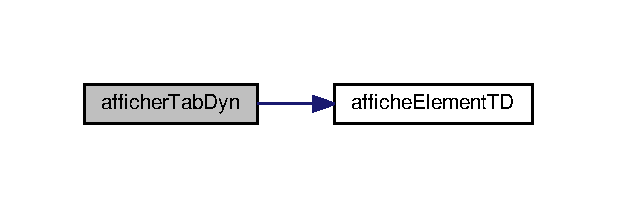
\includegraphics[width=296pt]{_jeu_8c_afd5a3bf829dfce68d6ee92c86bfe4a3c_cgraph}
\end{center}
\end{figure}


\hypertarget{_jeu_8c_a3389c806f79c54e7a4150967f604c7f7}{\index{Jeu.\-c@{Jeu.\-c}!ajouter\-Element\-Tab\-Dyn@{ajouter\-Element\-Tab\-Dyn}}
\index{ajouter\-Element\-Tab\-Dyn@{ajouter\-Element\-Tab\-Dyn}!Jeu.c@{Jeu.\-c}}
\subsubsection[{ajouter\-Element\-Tab\-Dyn}]{\setlength{\rightskip}{0pt plus 5cm}void ajouter\-Element\-Tab\-Dyn (
\begin{DoxyParamCaption}
\item[{{\bf Tableau\-Dynamique} $\ast$}]{t, }
\item[{{\bf Element\-T\-D}}]{e}
\end{DoxyParamCaption}
)}}\label{_jeu_8c_a3389c806f79c54e7a4150967f604c7f7}


ajouter\-Element\-Tab\-Dyn ajoute un element a la fin du tableau dynamique 


\begin{DoxyParams}{Parameters}
{\em Tableau\-Dynamique} & $\ast$t \\
\hline
{\em Element\-T\-D} & e \\
\hline
\end{DoxyParams}


Definition at line 396 of file Jeu.\-c.

\hypertarget{_jeu_8c_ad4612e76a9c8e5ecc0a4b70380b04a31}{\index{Jeu.\-c@{Jeu.\-c}!deplacer\-Projo@{deplacer\-Projo}}
\index{deplacer\-Projo@{deplacer\-Projo}!Jeu.c@{Jeu.\-c}}
\subsubsection[{deplacer\-Projo}]{\setlength{\rightskip}{0pt plus 5cm}void deplacer\-Projo (
\begin{DoxyParamCaption}
\item[{{\bf Jeu} $\ast$}]{, }
\item[{int}]{}
\end{DoxyParamCaption}
)}}\label{_jeu_8c_ad4612e76a9c8e5ecc0a4b70380b04a31}


deplacer\-Projo deplace le projectile 


\begin{DoxyParams}{Parameters}
{\em Jeu$\ast$} & \\
\hline
{\em int} & \\
\hline
\end{DoxyParams}


Definition at line 223 of file Jeu.\-c.

\hypertarget{_jeu_8c_a7518cb6d43b8202ba9a00bfe99fc3276}{\index{Jeu.\-c@{Jeu.\-c}!initialiser\-Tab\-Dyn@{initialiser\-Tab\-Dyn}}
\index{initialiser\-Tab\-Dyn@{initialiser\-Tab\-Dyn}!Jeu.c@{Jeu.\-c}}
\subsubsection[{initialiser\-Tab\-Dyn}]{\setlength{\rightskip}{0pt plus 5cm}void initialiser\-Tab\-Dyn (
\begin{DoxyParamCaption}
\item[{{\bf Tableau\-Dynamique} $\ast$}]{t}
\end{DoxyParamCaption}
)}}\label{_jeu_8c_a7518cb6d43b8202ba9a00bfe99fc3276}


initialiser\-Tab\-Dyn initialise un tableau dynamique 


\begin{DoxyParams}{Parameters}
{\em Tableau\-Dynamique} & $\ast$ t \\
\hline
\end{DoxyParams}


Definition at line 379 of file Jeu.\-c.

\hypertarget{_jeu_8c_a29bc8c099ab4b59464ab31a6f44a6465}{\index{Jeu.\-c@{Jeu.\-c}!init\-Projo@{init\-Projo}}
\index{init\-Projo@{init\-Projo}!Jeu.c@{Jeu.\-c}}
\subsubsection[{init\-Projo}]{\setlength{\rightskip}{0pt plus 5cm}void init\-Projo (
\begin{DoxyParamCaption}
\item[{{\bf Jeu} $\ast$}]{}
\end{DoxyParamCaption}
)}}\label{_jeu_8c_a29bc8c099ab4b59464ab31a6f44a6465}


init\-Projo initialise un nouveau projectile en fonction de l'orientation du personnage 


\begin{DoxyParams}{Parameters}
{\em Jeu$\ast$} & \\
\hline
\end{DoxyParams}


Definition at line 140 of file Jeu.\-c.



Here is the call graph for this function\-:\nopagebreak
\begin{figure}[H]
\begin{center}
\leavevmode
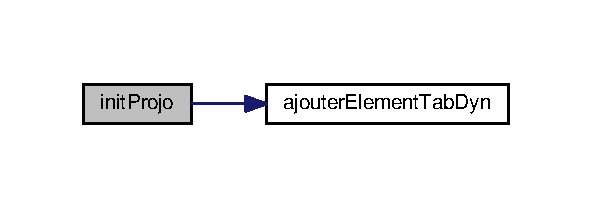
\includegraphics[width=284pt]{_jeu_8c_a29bc8c099ab4b59464ab31a6f44a6465_cgraph}
\end{center}
\end{figure}


\hypertarget{_jeu_8c_a0cf2f8d638bfab400e2c1b0103d87b62}{\index{Jeu.\-c@{Jeu.\-c}!init\-Projoclef@{init\-Projoclef}}
\index{init\-Projoclef@{init\-Projoclef}!Jeu.c@{Jeu.\-c}}
\subsubsection[{init\-Projoclef}]{\setlength{\rightskip}{0pt plus 5cm}void init\-Projoclef (
\begin{DoxyParamCaption}
\item[{{\bf Jeu} $\ast$}]{p\-Jeu}
\end{DoxyParamCaption}
)}}\label{_jeu_8c_a0cf2f8d638bfab400e2c1b0103d87b62}


Definition at line 214 of file Jeu.\-c.



Here is the call graph for this function\-:\nopagebreak
\begin{figure}[H]
\begin{center}
\leavevmode
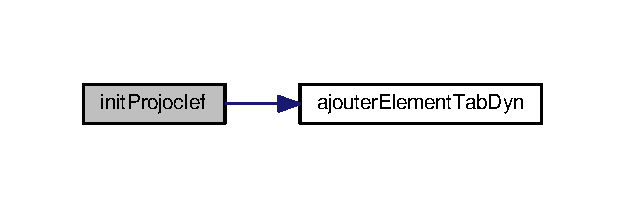
\includegraphics[width=300pt]{_jeu_8c_a0cf2f8d638bfab400e2c1b0103d87b62_cgraph}
\end{center}
\end{figure}


\hypertarget{_jeu_8c_a240e0a28446174a8ad0924c539e29c66}{\index{Jeu.\-c@{Jeu.\-c}!init\-Projohp@{init\-Projohp}}
\index{init\-Projohp@{init\-Projohp}!Jeu.c@{Jeu.\-c}}
\subsubsection[{init\-Projohp}]{\setlength{\rightskip}{0pt plus 5cm}void init\-Projohp (
\begin{DoxyParamCaption}
\item[{{\bf Jeu} $\ast$}]{p\-Jeu, }
\item[{int}]{i}
\end{DoxyParamCaption}
)}}\label{_jeu_8c_a240e0a28446174a8ad0924c539e29c66}


Definition at line 204 of file Jeu.\-c.



Here is the call graph for this function\-:\nopagebreak
\begin{figure}[H]
\begin{center}
\leavevmode
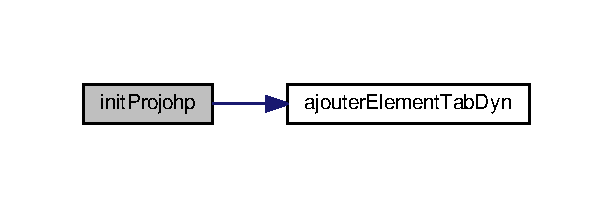
\includegraphics[width=294pt]{_jeu_8c_a240e0a28446174a8ad0924c539e29c66_cgraph}
\end{center}
\end{figure}


\hypertarget{_jeu_8c_a3c934fb69c2ca92e5e1f37dffac31df6}{\index{Jeu.\-c@{Jeu.\-c}!init\-Projo\-Rat@{init\-Projo\-Rat}}
\index{init\-Projo\-Rat@{init\-Projo\-Rat}!Jeu.c@{Jeu.\-c}}
\subsubsection[{init\-Projo\-Rat}]{\setlength{\rightskip}{0pt plus 5cm}void init\-Projo\-Rat (
\begin{DoxyParamCaption}
\item[{{\bf Jeu} $\ast$}]{p\-Jeu, }
\item[{int}]{i}
\end{DoxyParamCaption}
)}}\label{_jeu_8c_a3c934fb69c2ca92e5e1f37dffac31df6}


Definition at line 172 of file Jeu.\-c.



Here is the call graph for this function\-:\nopagebreak
\begin{figure}[H]
\begin{center}
\leavevmode
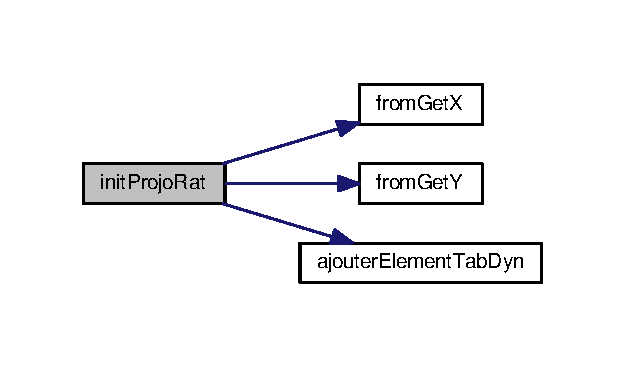
\includegraphics[width=300pt]{_jeu_8c_a3c934fb69c2ca92e5e1f37dffac31df6_cgraph}
\end{center}
\end{figure}


\hypertarget{_jeu_8c_a59334844989c7fb2edb6fbc3df80fe8b}{\index{Jeu.\-c@{Jeu.\-c}!jeu\-Action\-Clavier@{jeu\-Action\-Clavier}}
\index{jeu\-Action\-Clavier@{jeu\-Action\-Clavier}!Jeu.c@{Jeu.\-c}}
\subsubsection[{jeu\-Action\-Clavier}]{\setlength{\rightskip}{0pt plus 5cm}void jeu\-Action\-Clavier (
\begin{DoxyParamCaption}
\item[{{\bf Jeu} $\ast$}]{p\-Jeu, }
\item[{int}]{touche}
\end{DoxyParamCaption}
)}}\label{_jeu_8c_a59334844989c7fb2edb6fbc3df80fe8b}


Definition at line 68 of file Jeu.\-c.



Here is the call graph for this function\-:\nopagebreak
\begin{figure}[H]
\begin{center}
\leavevmode
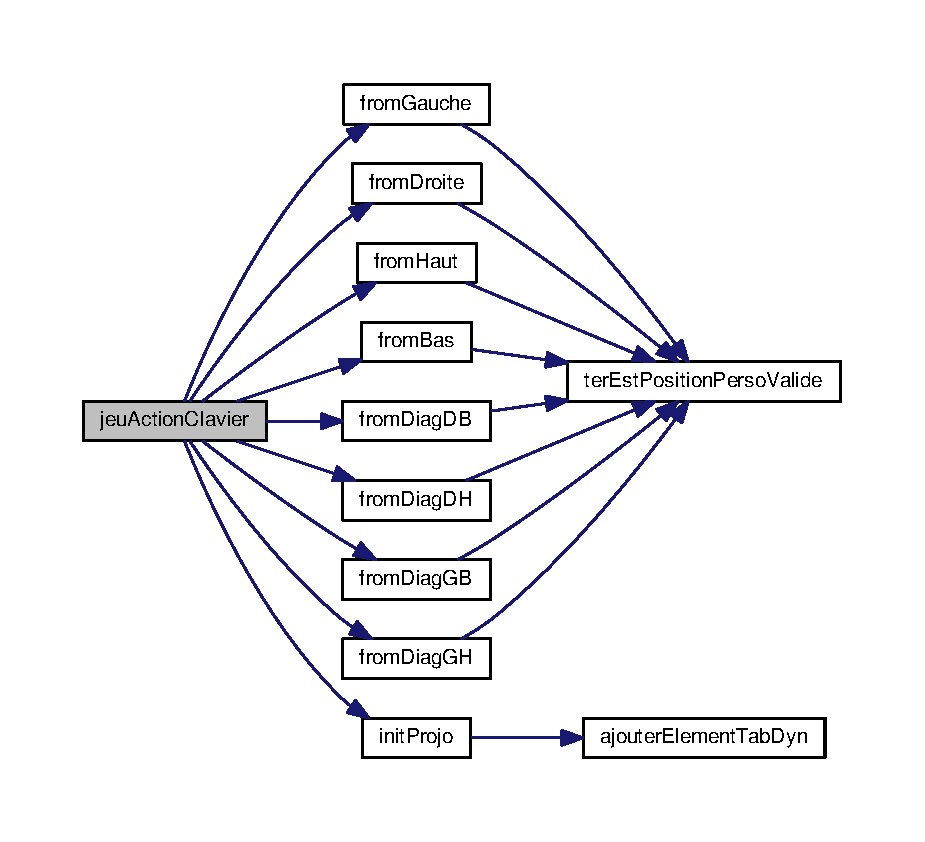
\includegraphics[width=350pt]{_jeu_8c_a59334844989c7fb2edb6fbc3df80fe8b_cgraph}
\end{center}
\end{figure}


\hypertarget{_jeu_8c_a352bd60c0d6e3d2d0293fde191b26b21}{\index{Jeu.\-c@{Jeu.\-c}!jeu\-Evolue@{jeu\-Evolue}}
\index{jeu\-Evolue@{jeu\-Evolue}!Jeu.c@{Jeu.\-c}}
\subsubsection[{jeu\-Evolue}]{\setlength{\rightskip}{0pt plus 5cm}void jeu\-Evolue (
\begin{DoxyParamCaption}
\item[{{\bf Jeu} $\ast$}]{p\-Jeu}
\end{DoxyParamCaption}
)}}\label{_jeu_8c_a352bd60c0d6e3d2d0293fde191b26b21}


Definition at line 265 of file Jeu.\-c.



Here is the call graph for this function\-:\nopagebreak
\begin{figure}[H]
\begin{center}
\leavevmode
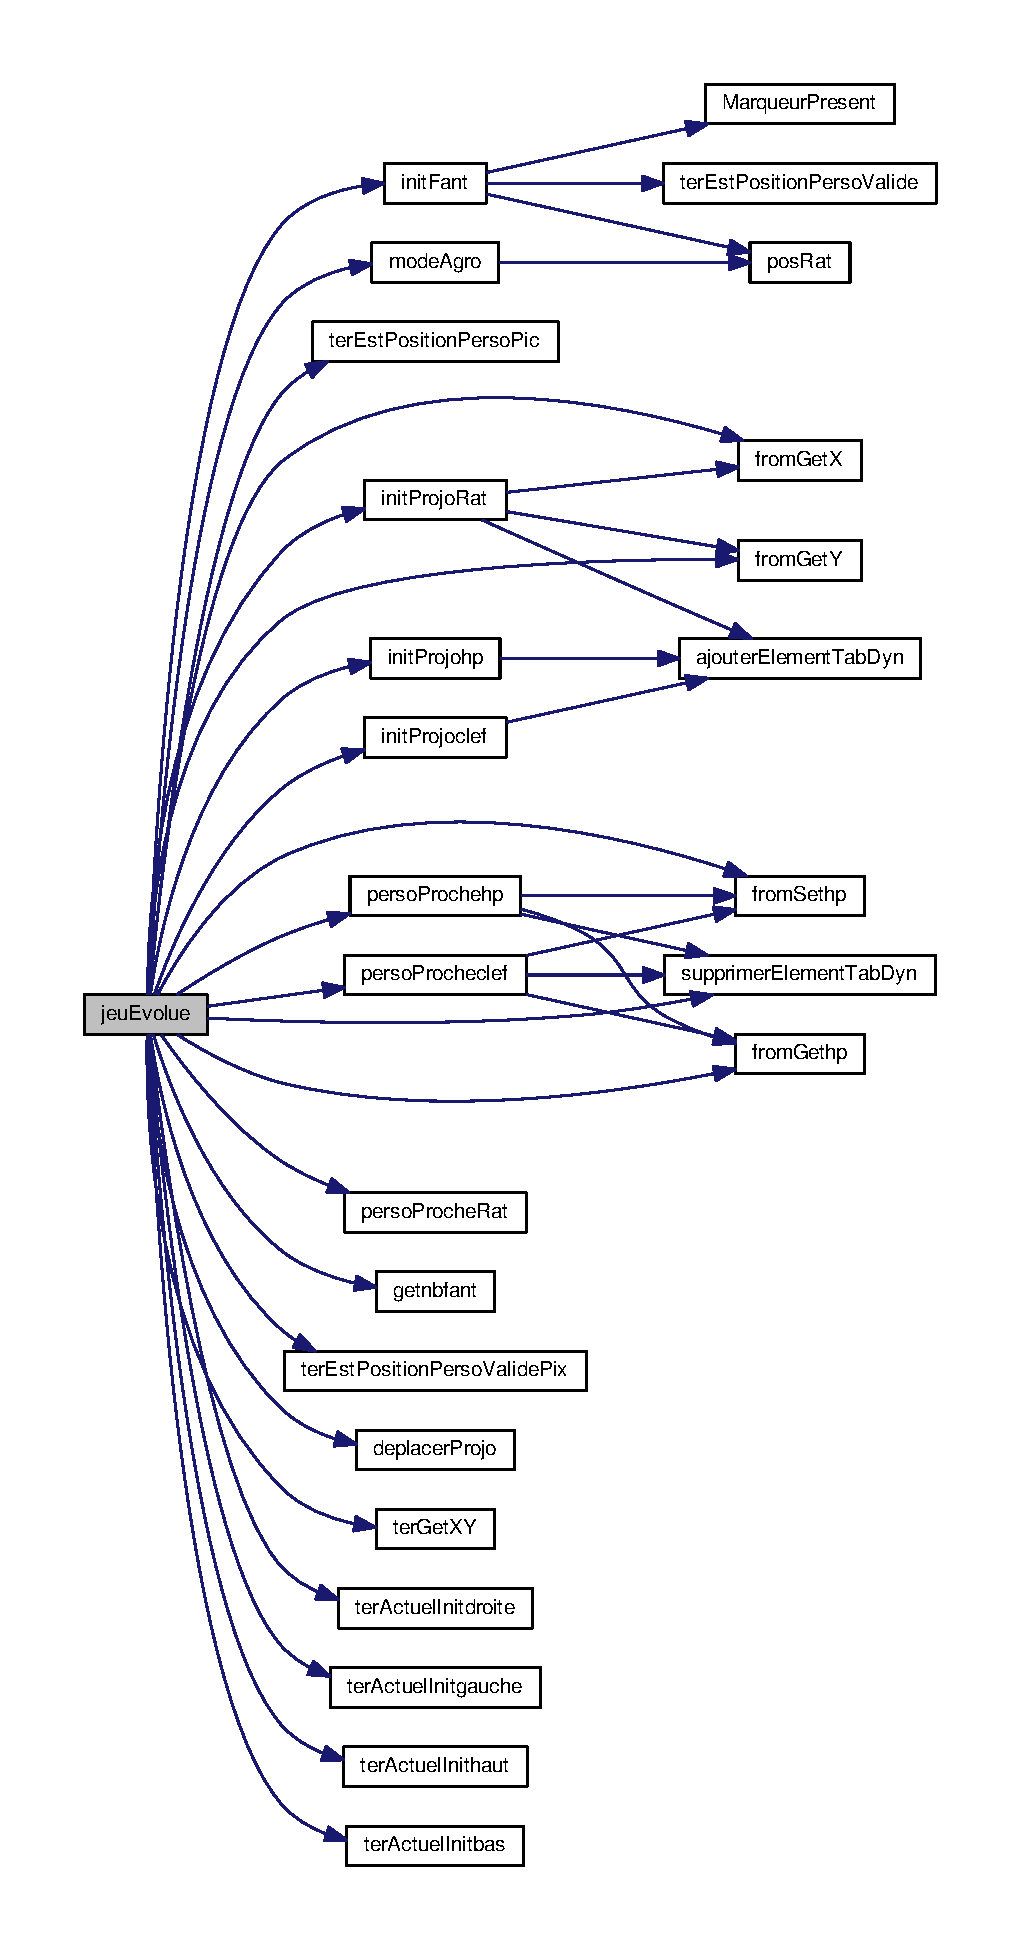
\includegraphics[height=550pt]{_jeu_8c_a352bd60c0d6e3d2d0293fde191b26b21_cgraph}
\end{center}
\end{figure}


\hypertarget{_jeu_8c_a2e878ce030a0a52788c7ee9ac2daeb55}{\index{Jeu.\-c@{Jeu.\-c}!jeu\-Get\-Const\-Fromage\-Ptr@{jeu\-Get\-Const\-Fromage\-Ptr}}
\index{jeu\-Get\-Const\-Fromage\-Ptr@{jeu\-Get\-Const\-Fromage\-Ptr}!Jeu.c@{Jeu.\-c}}
\subsubsection[{jeu\-Get\-Const\-Fromage\-Ptr}]{\setlength{\rightskip}{0pt plus 5cm}const {\bf Fromage}$\ast$ jeu\-Get\-Const\-Fromage\-Ptr (
\begin{DoxyParamCaption}
\item[{const {\bf Jeu} $\ast$}]{p\-Jeu}
\end{DoxyParamCaption}
)}}\label{_jeu_8c_a2e878ce030a0a52788c7ee9ac2daeb55}


Definition at line 54 of file Jeu.\-c.

\hypertarget{_jeu_8c_a2cbfcfb9733316dbc407c8a421285447}{\index{Jeu.\-c@{Jeu.\-c}!jeu\-Get\-Const\-Terrain\-Ptr@{jeu\-Get\-Const\-Terrain\-Ptr}}
\index{jeu\-Get\-Const\-Terrain\-Ptr@{jeu\-Get\-Const\-Terrain\-Ptr}!Jeu.c@{Jeu.\-c}}
\subsubsection[{jeu\-Get\-Const\-Terrain\-Ptr}]{\setlength{\rightskip}{0pt plus 5cm}const {\bf Terrain}$\ast$ jeu\-Get\-Const\-Terrain\-Ptr (
\begin{DoxyParamCaption}
\item[{const {\bf Jeu} $\ast$}]{p\-Jeu}
\end{DoxyParamCaption}
)}}\label{_jeu_8c_a2cbfcfb9733316dbc407c8a421285447}


Definition at line 49 of file Jeu.\-c.

\hypertarget{_jeu_8c_a62edb593072d6c43ba1b9362f0240058}{\index{Jeu.\-c@{Jeu.\-c}!jeu\-Get\-Fromage\-Ptr@{jeu\-Get\-Fromage\-Ptr}}
\index{jeu\-Get\-Fromage\-Ptr@{jeu\-Get\-Fromage\-Ptr}!Jeu.c@{Jeu.\-c}}
\subsubsection[{jeu\-Get\-Fromage\-Ptr}]{\setlength{\rightskip}{0pt plus 5cm}{\bf Fromage}$\ast$ jeu\-Get\-Fromage\-Ptr (
\begin{DoxyParamCaption}
\item[{{\bf Jeu} $\ast$}]{p\-Jeu}
\end{DoxyParamCaption}
)}}\label{_jeu_8c_a62edb593072d6c43ba1b9362f0240058}


Definition at line 44 of file Jeu.\-c.

\hypertarget{_jeu_8c_ae748f3f14e09a2f4b556545cef926394}{\index{Jeu.\-c@{Jeu.\-c}!jeu\-Get\-Terrain\-Ptr@{jeu\-Get\-Terrain\-Ptr}}
\index{jeu\-Get\-Terrain\-Ptr@{jeu\-Get\-Terrain\-Ptr}!Jeu.c@{Jeu.\-c}}
\subsubsection[{jeu\-Get\-Terrain\-Ptr}]{\setlength{\rightskip}{0pt plus 5cm}{\bf Terrain}$\ast$ jeu\-Get\-Terrain\-Ptr (
\begin{DoxyParamCaption}
\item[{{\bf Jeu} $\ast$}]{p\-Jeu}
\end{DoxyParamCaption}
)}}\label{_jeu_8c_ae748f3f14e09a2f4b556545cef926394}


Definition at line 39 of file Jeu.\-c.

\hypertarget{_jeu_8c_adea2de1f9bb9c58341d64db6e20261cc}{\index{Jeu.\-c@{Jeu.\-c}!jeu\-Init@{jeu\-Init}}
\index{jeu\-Init@{jeu\-Init}!Jeu.c@{Jeu.\-c}}
\subsubsection[{jeu\-Init}]{\setlength{\rightskip}{0pt plus 5cm}void jeu\-Init (
\begin{DoxyParamCaption}
\item[{{\bf Jeu} $\ast$}]{p\-Jeu}
\end{DoxyParamCaption}
)}}\label{_jeu_8c_adea2de1f9bb9c58341d64db6e20261cc}


Definition at line 24 of file Jeu.\-c.



Here is the call graph for this function\-:\nopagebreak
\begin{figure}[H]
\begin{center}
\leavevmode
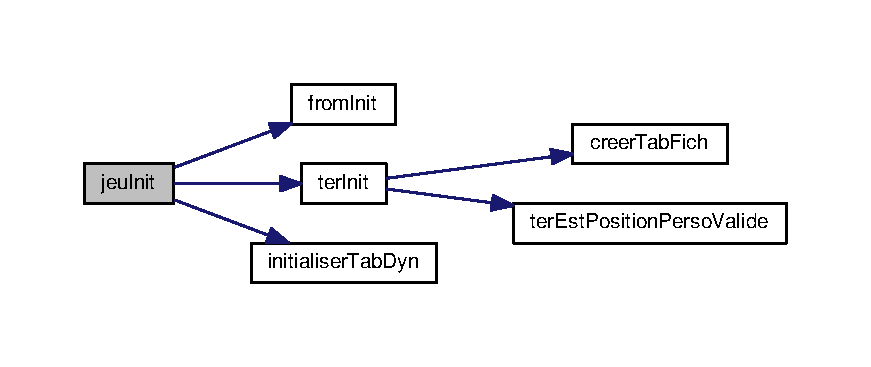
\includegraphics[width=350pt]{_jeu_8c_adea2de1f9bb9c58341d64db6e20261cc_cgraph}
\end{center}
\end{figure}


\hypertarget{_jeu_8c_a2ec855d639ca287ad8278b8baf49d677}{\index{Jeu.\-c@{Jeu.\-c}!jeu\-Libere@{jeu\-Libere}}
\index{jeu\-Libere@{jeu\-Libere}!Jeu.c@{Jeu.\-c}}
\subsubsection[{jeu\-Libere}]{\setlength{\rightskip}{0pt plus 5cm}void jeu\-Libere (
\begin{DoxyParamCaption}
\item[{{\bf Jeu} $\ast$}]{p\-Jeu}
\end{DoxyParamCaption}
)}}\label{_jeu_8c_a2ec855d639ca287ad8278b8baf49d677}


Definition at line 32 of file Jeu.\-c.



Here is the call graph for this function\-:\nopagebreak
\begin{figure}[H]
\begin{center}
\leavevmode
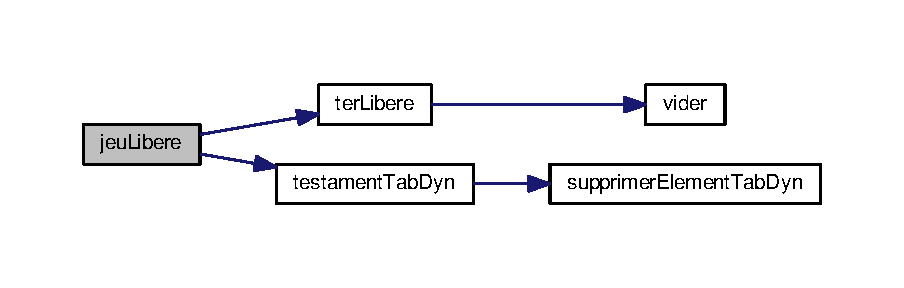
\includegraphics[width=350pt]{_jeu_8c_a2ec855d639ca287ad8278b8baf49d677_cgraph}
\end{center}
\end{figure}


\hypertarget{_jeu_8c_af54396488f24cbc0ea4c772b0a833be7}{\index{Jeu.\-c@{Jeu.\-c}!modifier\-Valeur\-Ieme\-Element\-Tab\-Dyn@{modifier\-Valeur\-Ieme\-Element\-Tab\-Dyn}}
\index{modifier\-Valeur\-Ieme\-Element\-Tab\-Dyn@{modifier\-Valeur\-Ieme\-Element\-Tab\-Dyn}!Jeu.c@{Jeu.\-c}}
\subsubsection[{modifier\-Valeur\-Ieme\-Element\-Tab\-Dyn}]{\setlength{\rightskip}{0pt plus 5cm}void modifier\-Valeur\-Ieme\-Element\-Tab\-Dyn (
\begin{DoxyParamCaption}
\item[{{\bf Tableau\-Dynamique} $\ast$}]{t, }
\item[{{\bf Element\-T\-D}}]{e, }
\item[{unsigned int}]{i}
\end{DoxyParamCaption}
)}}\label{_jeu_8c_af54396488f24cbc0ea4c772b0a833be7}


modifier\-Valeur\-Ieme\-Element\-Tab\-Dyn modifie l'ieme element du tableau dynamique par celui passer en parametre 


\begin{DoxyParams}{Parameters}
{\em Tableau\-Dynamique} & $\ast$t \\
\hline
{\em Element\-T\-D} & e \\
\hline
{\em unsigned} & int i \\
\hline
\end{DoxyParams}


Definition at line 464 of file Jeu.\-c.

\hypertarget{_jeu_8c_a52e4338b8a1c8e22017d66b9cad2af98}{\index{Jeu.\-c@{Jeu.\-c}!perso\-Procheclef@{perso\-Procheclef}}
\index{perso\-Procheclef@{perso\-Procheclef}!Jeu.c@{Jeu.\-c}}
\subsubsection[{perso\-Procheclef}]{\setlength{\rightskip}{0pt plus 5cm}void perso\-Procheclef (
\begin{DoxyParamCaption}
\item[{{\bf Jeu} $\ast$}]{p\-Jeu}
\end{DoxyParamCaption}
)}}\label{_jeu_8c_a52e4338b8a1c8e22017d66b9cad2af98}


Definition at line 252 of file Jeu.\-c.



Here is the call graph for this function\-:\nopagebreak
\begin{figure}[H]
\begin{center}
\leavevmode
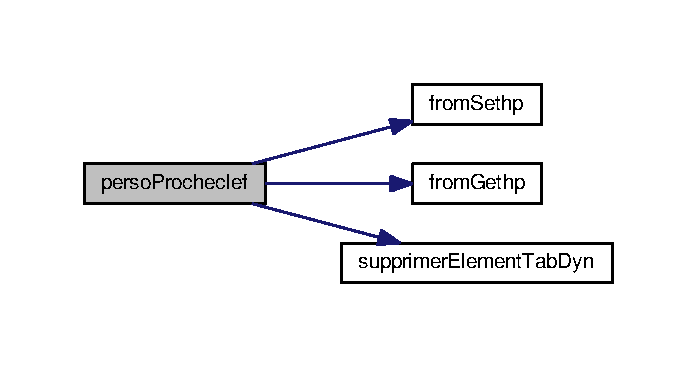
\includegraphics[width=334pt]{_jeu_8c_a52e4338b8a1c8e22017d66b9cad2af98_cgraph}
\end{center}
\end{figure}


\hypertarget{_jeu_8c_a92a6f56229e6e3bf17c627b9702b853d}{\index{Jeu.\-c@{Jeu.\-c}!perso\-Prochehp@{perso\-Prochehp}}
\index{perso\-Prochehp@{perso\-Prochehp}!Jeu.c@{Jeu.\-c}}
\subsubsection[{perso\-Prochehp}]{\setlength{\rightskip}{0pt plus 5cm}void perso\-Prochehp (
\begin{DoxyParamCaption}
\item[{{\bf Jeu} $\ast$}]{p\-Jeu}
\end{DoxyParamCaption}
)}}\label{_jeu_8c_a92a6f56229e6e3bf17c627b9702b853d}


Definition at line 240 of file Jeu.\-c.



Here is the call graph for this function\-:\nopagebreak
\begin{figure}[H]
\begin{center}
\leavevmode
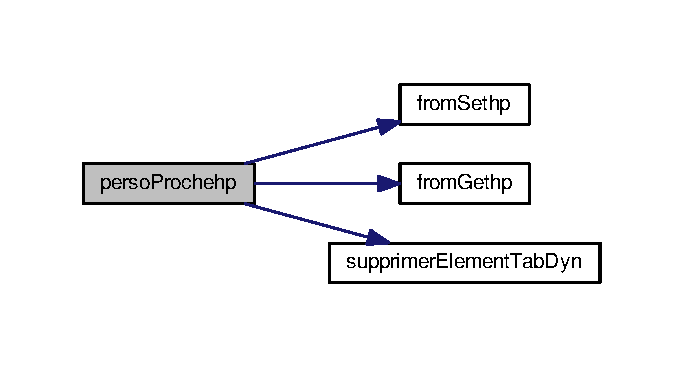
\includegraphics[width=328pt]{_jeu_8c_a92a6f56229e6e3bf17c627b9702b853d_cgraph}
\end{center}
\end{figure}


\hypertarget{_jeu_8c_a0d10365670f81c1e95814816e88ddcbf}{\index{Jeu.\-c@{Jeu.\-c}!supprimer\-Element\-Tab\-Dyn@{supprimer\-Element\-Tab\-Dyn}}
\index{supprimer\-Element\-Tab\-Dyn@{supprimer\-Element\-Tab\-Dyn}!Jeu.c@{Jeu.\-c}}
\subsubsection[{supprimer\-Element\-Tab\-Dyn}]{\setlength{\rightskip}{0pt plus 5cm}void supprimer\-Element\-Tab\-Dyn (
\begin{DoxyParamCaption}
\item[{{\bf Tableau\-Dynamique} $\ast$}]{t, }
\item[{int}]{position}
\end{DoxyParamCaption}
)}}\label{_jeu_8c_a0d10365670f81c1e95814816e88ddcbf}


supprimer\-Element\-Tab\-Dyn supprimme un element a la ieme position dans le tableau dynamique 


\begin{DoxyParams}{Parameters}
{\em Tableau\-Dynamique} & $\ast$t \\
\hline
{\em int} & position \\
\hline
\end{DoxyParams}


Definition at line 435 of file Jeu.\-c.

\hypertarget{_jeu_8c_a23c700cab62fac5e751c347b9248dc18}{\index{Jeu.\-c@{Jeu.\-c}!testament\-Tab\-Dyn@{testament\-Tab\-Dyn}}
\index{testament\-Tab\-Dyn@{testament\-Tab\-Dyn}!Jeu.c@{Jeu.\-c}}
\subsubsection[{testament\-Tab\-Dyn}]{\setlength{\rightskip}{0pt plus 5cm}void testament\-Tab\-Dyn (
\begin{DoxyParamCaption}
\item[{{\bf Tableau\-Dynamique} $\ast$}]{t}
\end{DoxyParamCaption}
)}}\label{_jeu_8c_a23c700cab62fac5e751c347b9248dc18}


testament\-Tab\-Dyn vide et libère un tableau dynamique 


\begin{DoxyParams}{Parameters}
{\em Tableau\-Dynamique} & $\ast$t \\
\hline
\end{DoxyParams}


Definition at line 386 of file Jeu.\-c.



Here is the call graph for this function\-:\nopagebreak
\begin{figure}[H]
\begin{center}
\leavevmode
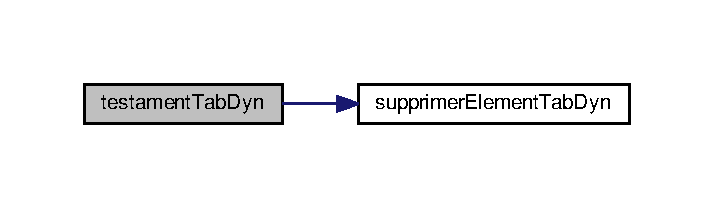
\includegraphics[width=342pt]{_jeu_8c_a23c700cab62fac5e751c347b9248dc18_cgraph}
\end{center}
\end{figure}


\hypertarget{_jeu_8c_a8801ebbe316e3da8e164162fa410466c}{\index{Jeu.\-c@{Jeu.\-c}!valeur\-Ieme\-Element\-Tab\-Dyn@{valeur\-Ieme\-Element\-Tab\-Dyn}}
\index{valeur\-Ieme\-Element\-Tab\-Dyn@{valeur\-Ieme\-Element\-Tab\-Dyn}!Jeu.c@{Jeu.\-c}}
\subsubsection[{valeur\-Ieme\-Element\-Tab\-Dyn}]{\setlength{\rightskip}{0pt plus 5cm}{\bf Element\-T\-D} valeur\-Ieme\-Element\-Tab\-Dyn (
\begin{DoxyParamCaption}
\item[{const {\bf Tableau\-Dynamique} $\ast$}]{t, }
\item[{unsigned int}]{i}
\end{DoxyParamCaption}
)}}\label{_jeu_8c_a8801ebbe316e3da8e164162fa410466c}


valeur\-Ieme\-Element\-Tab\-Dyn renvoie l'ieme element d'un tableau dynamique 


\begin{DoxyParams}{Parameters}
{\em const} & Tableau\-Dynamique $\ast$t \\
\hline
{\em unsigned} & int i \\
\hline
\end{DoxyParams}


Definition at line 416 of file Jeu.\-c.


\hypertarget{_jeu_8h}{\section{/home/enzo/projet\-\_\-fluide/src/\-Jeu.h File Reference}
\label{_jeu_8h}\index{/home/enzo/projet\-\_\-fluide/src/\-Jeu.\-h@{/home/enzo/projet\-\_\-fluide/src/\-Jeu.\-h}}
}
{\ttfamily \#include \char`\"{}Fromage.\-h\char`\"{}}\\*
{\ttfamily \#include \char`\"{}Terrain.\-h\char`\"{}}\\*
Include dependency graph for Jeu.\-h\-:\nopagebreak
\begin{figure}[H]
\begin{center}
\leavevmode
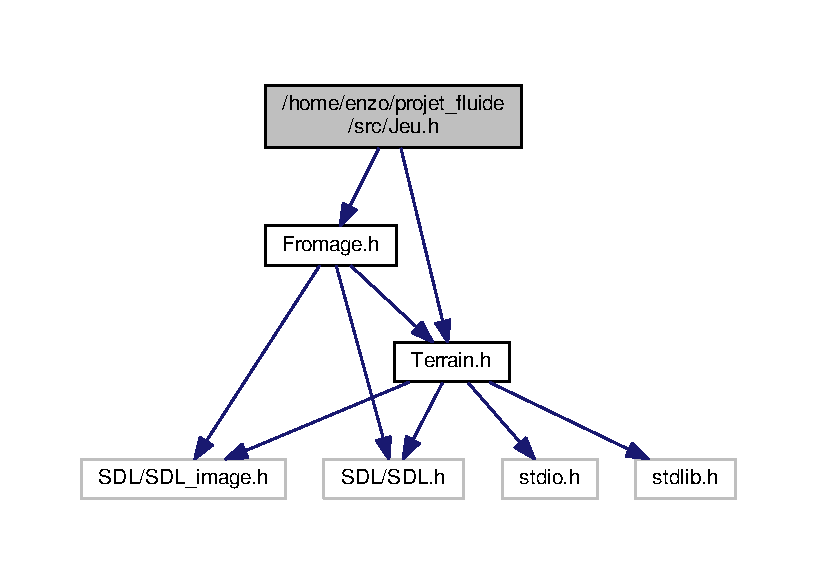
\includegraphics[width=350pt]{_jeu_8h__incl}
\end{center}
\end{figure}
This graph shows which files directly or indirectly include this file\-:
\nopagebreak
\begin{figure}[H]
\begin{center}
\leavevmode
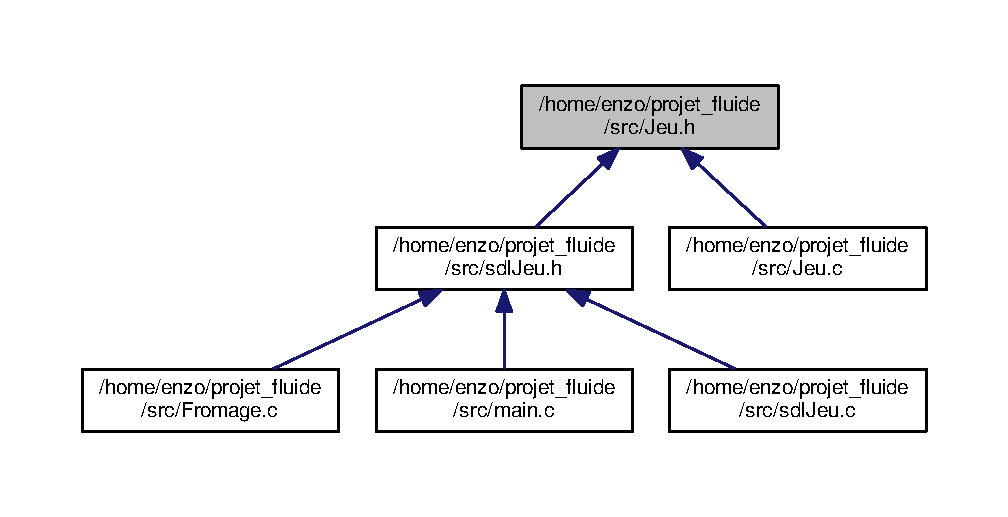
\includegraphics[width=350pt]{_jeu_8h__dep__incl}
\end{center}
\end{figure}
\subsection*{Data Structures}
\begin{DoxyCompactItemize}
\item 
struct \hyperlink{struct_projectile}{Projectile}
\item 
struct \hyperlink{structs_tableau_dynamique}{s\-Tableau\-Dynamique}
\item 
struct \hyperlink{struct_jeu}{Jeu}
\end{DoxyCompactItemize}
\subsection*{Typedefs}
\begin{DoxyCompactItemize}
\item 
typedef \hyperlink{struct_projectile}{Projectile} \hyperlink{_jeu_8h_a19f385bd48e6eaff3c61e8abf073263e}{Element\-T\-D}
\item 
typedef struct \hyperlink{structs_tableau_dynamique}{s\-Tableau\-Dynamique} \hyperlink{_jeu_8h_a8248fdbab1c5aa4232c53c2f209f989a}{Tableau\-Dynamique}
\end{DoxyCompactItemize}
\subsection*{Functions}
\begin{DoxyCompactItemize}
\item 
void \hyperlink{_jeu_8h_a3e31ce457d0c1a4c9723a4b699d48a84}{init\-Projo} (\hyperlink{struct_jeu}{Jeu} $\ast$)
\begin{DoxyCompactList}\small\item\em init\-Projo initialise un nouveau projectile en fonction de l'orientation du personnage \end{DoxyCompactList}\item 
void \hyperlink{_jeu_8h_ae7000fd1b75f52155d56828cb6b10989}{deplacer\-Projo} (\hyperlink{struct_jeu}{Jeu} $\ast$, int)
\begin{DoxyCompactList}\small\item\em deplacer\-Projo deplace le projectile \end{DoxyCompactList}\item 
void \hyperlink{_jeu_8h_a7518cb6d43b8202ba9a00bfe99fc3276}{initialiser\-Tab\-Dyn} (\hyperlink{_jeu_8h_a8248fdbab1c5aa4232c53c2f209f989a}{Tableau\-Dynamique} $\ast$t)
\begin{DoxyCompactList}\small\item\em initialiser\-Tab\-Dyn initialise un tableau dynamique \end{DoxyCompactList}\item 
void \hyperlink{_jeu_8h_a23c700cab62fac5e751c347b9248dc18}{testament\-Tab\-Dyn} (\hyperlink{_jeu_8h_a8248fdbab1c5aa4232c53c2f209f989a}{Tableau\-Dynamique} $\ast$t)
\begin{DoxyCompactList}\small\item\em testament\-Tab\-Dyn vide et libère un tableau dynamique \end{DoxyCompactList}\item 
void \hyperlink{_jeu_8h_ae62c34e693110e9e5a159769505059b1}{affecter\-Tab\-Dyn} (\hyperlink{_jeu_8h_a8248fdbab1c5aa4232c53c2f209f989a}{Tableau\-Dynamique} $\ast$t1, const \hyperlink{_jeu_8h_a8248fdbab1c5aa4232c53c2f209f989a}{Tableau\-Dynamique} $\ast$t2)
\begin{DoxyCompactList}\small\item\em affecter\-Tab\-Dyn affecte un tableau dynamique dans un nouveau tableau dynamique \end{DoxyCompactList}\item 
unsigned int \hyperlink{_jeu_8h_a88c6d8f56e71ed8e6d7196cd74f40cb6}{taille\-Utilisee\-Tab\-Dyn} (const \hyperlink{_jeu_8h_a8248fdbab1c5aa4232c53c2f209f989a}{Tableau\-Dynamique} $\ast$t)
\begin{DoxyCompactList}\small\item\em taille\-Utilisee\-Tab\-Dyn renvoie la taille utilisée par un tableau dynamique \end{DoxyCompactList}\item 
\hyperlink{_jeu_8h_a19f385bd48e6eaff3c61e8abf073263e}{Element\-T\-D} \hyperlink{_jeu_8h_a8801ebbe316e3da8e164162fa410466c}{valeur\-Ieme\-Element\-Tab\-Dyn} (const \hyperlink{_jeu_8h_a8248fdbab1c5aa4232c53c2f209f989a}{Tableau\-Dynamique} $\ast$t, unsigned int i)
\begin{DoxyCompactList}\small\item\em valeur\-Ieme\-Element\-Tab\-Dyn renvoie l'ieme element d'un tableau dynamique \end{DoxyCompactList}\item 
void \hyperlink{_jeu_8h_afd5a3bf829dfce68d6ee92c86bfe4a3c}{afficher\-Tab\-Dyn} (const \hyperlink{_jeu_8h_a8248fdbab1c5aa4232c53c2f209f989a}{Tableau\-Dynamique} $\ast$t)
\begin{DoxyCompactList}\small\item\em afficher\-Tab\-Dyn affiche les elements du tableau dynamique \end{DoxyCompactList}\item 
void \hyperlink{_jeu_8h_a3389c806f79c54e7a4150967f604c7f7}{ajouter\-Element\-Tab\-Dyn} (\hyperlink{_jeu_8h_a8248fdbab1c5aa4232c53c2f209f989a}{Tableau\-Dynamique} $\ast$t, \hyperlink{_jeu_8h_a19f385bd48e6eaff3c61e8abf073263e}{Element\-T\-D} e)
\begin{DoxyCompactList}\small\item\em ajouter\-Element\-Tab\-Dyn ajoute un element a la fin du tableau dynamique \end{DoxyCompactList}\item 
void \hyperlink{_jeu_8h_a0d10365670f81c1e95814816e88ddcbf}{supprimer\-Element\-Tab\-Dyn} (\hyperlink{_jeu_8h_a8248fdbab1c5aa4232c53c2f209f989a}{Tableau\-Dynamique} $\ast$t, int position)
\begin{DoxyCompactList}\small\item\em supprimer\-Element\-Tab\-Dyn supprimme un element a la ieme position dans le tableau dynamique \end{DoxyCompactList}\item 
void \hyperlink{_jeu_8h_af54396488f24cbc0ea4c772b0a833be7}{modifier\-Valeur\-Ieme\-Element\-Tab\-Dyn} (\hyperlink{_jeu_8h_a8248fdbab1c5aa4232c53c2f209f989a}{Tableau\-Dynamique} $\ast$t, \hyperlink{_jeu_8h_a19f385bd48e6eaff3c61e8abf073263e}{Element\-T\-D} e, unsigned int i)
\begin{DoxyCompactList}\small\item\em modifier\-Valeur\-Ieme\-Element\-Tab\-Dyn modifie l'ieme element du tableau dynamique par celui passer en parametre \end{DoxyCompactList}\item 
void \hyperlink{_jeu_8h_a8032aaa63ec6b2231f3ac50a5da6eddb}{inserer\-Element\-Tab\-Dyn} (\hyperlink{_jeu_8h_a8248fdbab1c5aa4232c53c2f209f989a}{Tableau\-Dynamique} $\ast$t, \hyperlink{_jeu_8h_a19f385bd48e6eaff3c61e8abf073263e}{Element\-T\-D} e, unsigned int i)
\begin{DoxyCompactList}\small\item\em inserer\-Element\-Tab\-Dyn insere l'element passer en parametre a la ieme place du tableau dynamique \end{DoxyCompactList}\item 
void \hyperlink{_jeu_8h_aaa7f56dc206507579b5140e05cd278a2}{trier\-Tab\-Dyn} (\hyperlink{_jeu_8h_a8248fdbab1c5aa4232c53c2f209f989a}{Tableau\-Dynamique} $\ast$t)
\begin{DoxyCompactList}\small\item\em trier\-Tab\-Dyn trie un tableau dynamique \end{DoxyCompactList}\item 
int \hyperlink{_jeu_8h_a708b88c428cdc2cfe963934ebcca3132}{rechercher\-Element\-Tab\-Dyn} (const \hyperlink{_jeu_8h_a8248fdbab1c5aa4232c53c2f209f989a}{Tableau\-Dynamique} $\ast$t, \hyperlink{_jeu_8h_a19f385bd48e6eaff3c61e8abf073263e}{Element\-T\-D} e)
\begin{DoxyCompactList}\small\item\em rechercher\-Element\-Tab\-Dyn cherche et renvoie l'element passer en parametre \end{DoxyCompactList}\end{DoxyCompactItemize}


\subsection{Typedef Documentation}
\hypertarget{_jeu_8h_a19f385bd48e6eaff3c61e8abf073263e}{\index{Jeu.\-h@{Jeu.\-h}!Element\-T\-D@{Element\-T\-D}}
\index{Element\-T\-D@{Element\-T\-D}!Jeu.h@{Jeu.\-h}}
\subsubsection[{Element\-T\-D}]{\setlength{\rightskip}{0pt plus 5cm}typedef {\bf Projectile} {\bf Element\-T\-D}}}\label{_jeu_8h_a19f385bd48e6eaff3c61e8abf073263e}


Definition at line 11 of file Jeu.\-h.

\hypertarget{_jeu_8h_a8248fdbab1c5aa4232c53c2f209f989a}{\index{Jeu.\-h@{Jeu.\-h}!Tableau\-Dynamique@{Tableau\-Dynamique}}
\index{Tableau\-Dynamique@{Tableau\-Dynamique}!Jeu.h@{Jeu.\-h}}
\subsubsection[{Tableau\-Dynamique}]{\setlength{\rightskip}{0pt plus 5cm}typedef struct {\bf s\-Tableau\-Dynamique} {\bf Tableau\-Dynamique}}}\label{_jeu_8h_a8248fdbab1c5aa4232c53c2f209f989a}


Definition at line 19 of file Jeu.\-h.



\subsection{Function Documentation}
\hypertarget{_jeu_8h_ae62c34e693110e9e5a159769505059b1}{\index{Jeu.\-h@{Jeu.\-h}!affecter\-Tab\-Dyn@{affecter\-Tab\-Dyn}}
\index{affecter\-Tab\-Dyn@{affecter\-Tab\-Dyn}!Jeu.h@{Jeu.\-h}}
\subsubsection[{affecter\-Tab\-Dyn}]{\setlength{\rightskip}{0pt plus 5cm}void affecter\-Tab\-Dyn (
\begin{DoxyParamCaption}
\item[{{\bf Tableau\-Dynamique} $\ast$}]{t1, }
\item[{const {\bf Tableau\-Dynamique} $\ast$}]{t2}
\end{DoxyParamCaption}
)}}\label{_jeu_8h_ae62c34e693110e9e5a159769505059b1}


affecter\-Tab\-Dyn affecte un tableau dynamique dans un nouveau tableau dynamique 


\begin{DoxyParams}{Parameters}
{\em Tableau\-Dynamique} & $\ast$t1 \\
\hline
{\em const} & Tableau\-Dynamique $\ast$t2 \\
\hline
\end{DoxyParams}
\hypertarget{_jeu_8h_afd5a3bf829dfce68d6ee92c86bfe4a3c}{\index{Jeu.\-h@{Jeu.\-h}!afficher\-Tab\-Dyn@{afficher\-Tab\-Dyn}}
\index{afficher\-Tab\-Dyn@{afficher\-Tab\-Dyn}!Jeu.h@{Jeu.\-h}}
\subsubsection[{afficher\-Tab\-Dyn}]{\setlength{\rightskip}{0pt plus 5cm}void afficher\-Tab\-Dyn (
\begin{DoxyParamCaption}
\item[{const {\bf Tableau\-Dynamique} $\ast$}]{t}
\end{DoxyParamCaption}
)}}\label{_jeu_8h_afd5a3bf829dfce68d6ee92c86bfe4a3c}


afficher\-Tab\-Dyn affiche les elements du tableau dynamique 


\begin{DoxyParams}{Parameters}
{\em const} & Tableau\-Dynamique $\ast$t \\
\hline
\end{DoxyParams}


Definition at line 423 of file Jeu.\-c.



Here is the call graph for this function\-:\nopagebreak
\begin{figure}[H]
\begin{center}
\leavevmode
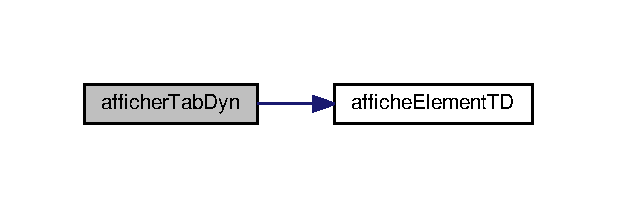
\includegraphics[width=296pt]{_jeu_8h_afd5a3bf829dfce68d6ee92c86bfe4a3c_cgraph}
\end{center}
\end{figure}


\hypertarget{_jeu_8h_a3389c806f79c54e7a4150967f604c7f7}{\index{Jeu.\-h@{Jeu.\-h}!ajouter\-Element\-Tab\-Dyn@{ajouter\-Element\-Tab\-Dyn}}
\index{ajouter\-Element\-Tab\-Dyn@{ajouter\-Element\-Tab\-Dyn}!Jeu.h@{Jeu.\-h}}
\subsubsection[{ajouter\-Element\-Tab\-Dyn}]{\setlength{\rightskip}{0pt plus 5cm}void ajouter\-Element\-Tab\-Dyn (
\begin{DoxyParamCaption}
\item[{{\bf Tableau\-Dynamique} $\ast$}]{t, }
\item[{{\bf Element\-T\-D}}]{e}
\end{DoxyParamCaption}
)}}\label{_jeu_8h_a3389c806f79c54e7a4150967f604c7f7}


ajouter\-Element\-Tab\-Dyn ajoute un element a la fin du tableau dynamique 


\begin{DoxyParams}{Parameters}
{\em Tableau\-Dynamique} & $\ast$t \\
\hline
{\em Element\-T\-D} & e \\
\hline
\end{DoxyParams}


Definition at line 396 of file Jeu.\-c.

\hypertarget{_jeu_8h_ae7000fd1b75f52155d56828cb6b10989}{\index{Jeu.\-h@{Jeu.\-h}!deplacer\-Projo@{deplacer\-Projo}}
\index{deplacer\-Projo@{deplacer\-Projo}!Jeu.h@{Jeu.\-h}}
\subsubsection[{deplacer\-Projo}]{\setlength{\rightskip}{0pt plus 5cm}void deplacer\-Projo (
\begin{DoxyParamCaption}
\item[{{\bf Jeu} $\ast$}]{, }
\item[{int}]{}
\end{DoxyParamCaption}
)}}\label{_jeu_8h_ae7000fd1b75f52155d56828cb6b10989}


deplacer\-Projo deplace le projectile 


\begin{DoxyParams}{Parameters}
{\em Jeu$\ast$} & \\
\hline
{\em int} & \\
\hline
\end{DoxyParams}


Definition at line 223 of file Jeu.\-c.

\hypertarget{_jeu_8h_a7518cb6d43b8202ba9a00bfe99fc3276}{\index{Jeu.\-h@{Jeu.\-h}!initialiser\-Tab\-Dyn@{initialiser\-Tab\-Dyn}}
\index{initialiser\-Tab\-Dyn@{initialiser\-Tab\-Dyn}!Jeu.h@{Jeu.\-h}}
\subsubsection[{initialiser\-Tab\-Dyn}]{\setlength{\rightskip}{0pt plus 5cm}void initialiser\-Tab\-Dyn (
\begin{DoxyParamCaption}
\item[{{\bf Tableau\-Dynamique} $\ast$}]{t}
\end{DoxyParamCaption}
)}}\label{_jeu_8h_a7518cb6d43b8202ba9a00bfe99fc3276}


initialiser\-Tab\-Dyn initialise un tableau dynamique 


\begin{DoxyParams}{Parameters}
{\em Tableau\-Dynamique} & $\ast$ t \\
\hline
\end{DoxyParams}


Definition at line 379 of file Jeu.\-c.

\hypertarget{_jeu_8h_a3e31ce457d0c1a4c9723a4b699d48a84}{\index{Jeu.\-h@{Jeu.\-h}!init\-Projo@{init\-Projo}}
\index{init\-Projo@{init\-Projo}!Jeu.h@{Jeu.\-h}}
\subsubsection[{init\-Projo}]{\setlength{\rightskip}{0pt plus 5cm}void init\-Projo (
\begin{DoxyParamCaption}
\item[{{\bf Jeu} $\ast$}]{}
\end{DoxyParamCaption}
)}}\label{_jeu_8h_a3e31ce457d0c1a4c9723a4b699d48a84}


init\-Projo initialise un nouveau projectile en fonction de l'orientation du personnage 


\begin{DoxyParams}{Parameters}
{\em Jeu$\ast$} & \\
\hline
\end{DoxyParams}


Definition at line 140 of file Jeu.\-c.



Here is the call graph for this function\-:\nopagebreak
\begin{figure}[H]
\begin{center}
\leavevmode
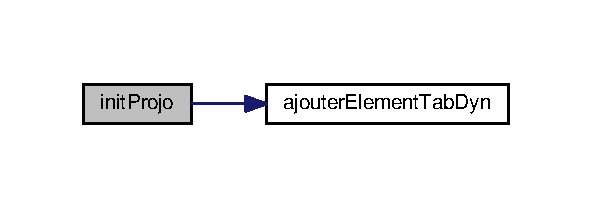
\includegraphics[width=284pt]{_jeu_8h_a3e31ce457d0c1a4c9723a4b699d48a84_cgraph}
\end{center}
\end{figure}


\hypertarget{_jeu_8h_a8032aaa63ec6b2231f3ac50a5da6eddb}{\index{Jeu.\-h@{Jeu.\-h}!inserer\-Element\-Tab\-Dyn@{inserer\-Element\-Tab\-Dyn}}
\index{inserer\-Element\-Tab\-Dyn@{inserer\-Element\-Tab\-Dyn}!Jeu.h@{Jeu.\-h}}
\subsubsection[{inserer\-Element\-Tab\-Dyn}]{\setlength{\rightskip}{0pt plus 5cm}void inserer\-Element\-Tab\-Dyn (
\begin{DoxyParamCaption}
\item[{{\bf Tableau\-Dynamique} $\ast$}]{t, }
\item[{{\bf Element\-T\-D}}]{e, }
\item[{unsigned int}]{i}
\end{DoxyParamCaption}
)}}\label{_jeu_8h_a8032aaa63ec6b2231f3ac50a5da6eddb}


inserer\-Element\-Tab\-Dyn insere l'element passer en parametre a la ieme place du tableau dynamique 


\begin{DoxyParams}{Parameters}
{\em Tableau\-Dynamique} & $\ast$t \\
\hline
{\em Element\-T\-D} & e \\
\hline
{\em unsigned} & int i \\
\hline
\end{DoxyParams}
\hypertarget{_jeu_8h_af54396488f24cbc0ea4c772b0a833be7}{\index{Jeu.\-h@{Jeu.\-h}!modifier\-Valeur\-Ieme\-Element\-Tab\-Dyn@{modifier\-Valeur\-Ieme\-Element\-Tab\-Dyn}}
\index{modifier\-Valeur\-Ieme\-Element\-Tab\-Dyn@{modifier\-Valeur\-Ieme\-Element\-Tab\-Dyn}!Jeu.h@{Jeu.\-h}}
\subsubsection[{modifier\-Valeur\-Ieme\-Element\-Tab\-Dyn}]{\setlength{\rightskip}{0pt plus 5cm}void modifier\-Valeur\-Ieme\-Element\-Tab\-Dyn (
\begin{DoxyParamCaption}
\item[{{\bf Tableau\-Dynamique} $\ast$}]{t, }
\item[{{\bf Element\-T\-D}}]{e, }
\item[{unsigned int}]{i}
\end{DoxyParamCaption}
)}}\label{_jeu_8h_af54396488f24cbc0ea4c772b0a833be7}


modifier\-Valeur\-Ieme\-Element\-Tab\-Dyn modifie l'ieme element du tableau dynamique par celui passer en parametre 


\begin{DoxyParams}{Parameters}
{\em Tableau\-Dynamique} & $\ast$t \\
\hline
{\em Element\-T\-D} & e \\
\hline
{\em unsigned} & int i \\
\hline
\end{DoxyParams}


Definition at line 464 of file Jeu.\-c.

\hypertarget{_jeu_8h_a708b88c428cdc2cfe963934ebcca3132}{\index{Jeu.\-h@{Jeu.\-h}!rechercher\-Element\-Tab\-Dyn@{rechercher\-Element\-Tab\-Dyn}}
\index{rechercher\-Element\-Tab\-Dyn@{rechercher\-Element\-Tab\-Dyn}!Jeu.h@{Jeu.\-h}}
\subsubsection[{rechercher\-Element\-Tab\-Dyn}]{\setlength{\rightskip}{0pt plus 5cm}int rechercher\-Element\-Tab\-Dyn (
\begin{DoxyParamCaption}
\item[{const {\bf Tableau\-Dynamique} $\ast$}]{t, }
\item[{{\bf Element\-T\-D}}]{e}
\end{DoxyParamCaption}
)}}\label{_jeu_8h_a708b88c428cdc2cfe963934ebcca3132}


rechercher\-Element\-Tab\-Dyn cherche et renvoie l'element passer en parametre 


\begin{DoxyParams}{Parameters}
{\em const} & Tableau\-Dynamique $\ast$t \\
\hline
{\em Element\-T\-D} & e \\
\hline
\end{DoxyParams}
\hypertarget{_jeu_8h_a0d10365670f81c1e95814816e88ddcbf}{\index{Jeu.\-h@{Jeu.\-h}!supprimer\-Element\-Tab\-Dyn@{supprimer\-Element\-Tab\-Dyn}}
\index{supprimer\-Element\-Tab\-Dyn@{supprimer\-Element\-Tab\-Dyn}!Jeu.h@{Jeu.\-h}}
\subsubsection[{supprimer\-Element\-Tab\-Dyn}]{\setlength{\rightskip}{0pt plus 5cm}void supprimer\-Element\-Tab\-Dyn (
\begin{DoxyParamCaption}
\item[{{\bf Tableau\-Dynamique} $\ast$}]{t, }
\item[{int}]{position}
\end{DoxyParamCaption}
)}}\label{_jeu_8h_a0d10365670f81c1e95814816e88ddcbf}


supprimer\-Element\-Tab\-Dyn supprimme un element a la ieme position dans le tableau dynamique 


\begin{DoxyParams}{Parameters}
{\em Tableau\-Dynamique} & $\ast$t \\
\hline
{\em int} & position \\
\hline
\end{DoxyParams}


Definition at line 435 of file Jeu.\-c.

\hypertarget{_jeu_8h_a88c6d8f56e71ed8e6d7196cd74f40cb6}{\index{Jeu.\-h@{Jeu.\-h}!taille\-Utilisee\-Tab\-Dyn@{taille\-Utilisee\-Tab\-Dyn}}
\index{taille\-Utilisee\-Tab\-Dyn@{taille\-Utilisee\-Tab\-Dyn}!Jeu.h@{Jeu.\-h}}
\subsubsection[{taille\-Utilisee\-Tab\-Dyn}]{\setlength{\rightskip}{0pt plus 5cm}unsigned int taille\-Utilisee\-Tab\-Dyn (
\begin{DoxyParamCaption}
\item[{const {\bf Tableau\-Dynamique} $\ast$}]{t}
\end{DoxyParamCaption}
)}}\label{_jeu_8h_a88c6d8f56e71ed8e6d7196cd74f40cb6}


taille\-Utilisee\-Tab\-Dyn renvoie la taille utilisée par un tableau dynamique 


\begin{DoxyParams}{Parameters}
{\em const} & Tableau\-Dynamique $\ast$t \\
\hline
\end{DoxyParams}
\hypertarget{_jeu_8h_a23c700cab62fac5e751c347b9248dc18}{\index{Jeu.\-h@{Jeu.\-h}!testament\-Tab\-Dyn@{testament\-Tab\-Dyn}}
\index{testament\-Tab\-Dyn@{testament\-Tab\-Dyn}!Jeu.h@{Jeu.\-h}}
\subsubsection[{testament\-Tab\-Dyn}]{\setlength{\rightskip}{0pt plus 5cm}void testament\-Tab\-Dyn (
\begin{DoxyParamCaption}
\item[{{\bf Tableau\-Dynamique} $\ast$}]{t}
\end{DoxyParamCaption}
)}}\label{_jeu_8h_a23c700cab62fac5e751c347b9248dc18}


testament\-Tab\-Dyn vide et libère un tableau dynamique 


\begin{DoxyParams}{Parameters}
{\em Tableau\-Dynamique} & $\ast$t \\
\hline
\end{DoxyParams}


Definition at line 386 of file Jeu.\-c.



Here is the call graph for this function\-:\nopagebreak
\begin{figure}[H]
\begin{center}
\leavevmode
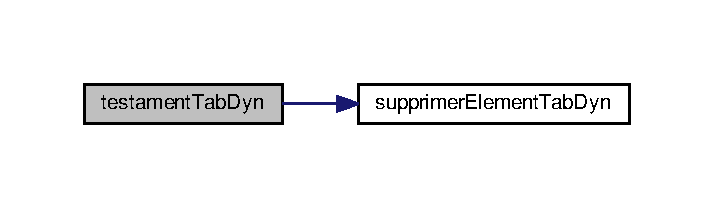
\includegraphics[width=342pt]{_jeu_8h_a23c700cab62fac5e751c347b9248dc18_cgraph}
\end{center}
\end{figure}


\hypertarget{_jeu_8h_aaa7f56dc206507579b5140e05cd278a2}{\index{Jeu.\-h@{Jeu.\-h}!trier\-Tab\-Dyn@{trier\-Tab\-Dyn}}
\index{trier\-Tab\-Dyn@{trier\-Tab\-Dyn}!Jeu.h@{Jeu.\-h}}
\subsubsection[{trier\-Tab\-Dyn}]{\setlength{\rightskip}{0pt plus 5cm}void trier\-Tab\-Dyn (
\begin{DoxyParamCaption}
\item[{{\bf Tableau\-Dynamique} $\ast$}]{t}
\end{DoxyParamCaption}
)}}\label{_jeu_8h_aaa7f56dc206507579b5140e05cd278a2}


trier\-Tab\-Dyn trie un tableau dynamique 


\begin{DoxyParams}{Parameters}
{\em Tableau\-Dynamique} & $\ast$t \\
\hline
\end{DoxyParams}
\hypertarget{_jeu_8h_a8801ebbe316e3da8e164162fa410466c}{\index{Jeu.\-h@{Jeu.\-h}!valeur\-Ieme\-Element\-Tab\-Dyn@{valeur\-Ieme\-Element\-Tab\-Dyn}}
\index{valeur\-Ieme\-Element\-Tab\-Dyn@{valeur\-Ieme\-Element\-Tab\-Dyn}!Jeu.h@{Jeu.\-h}}
\subsubsection[{valeur\-Ieme\-Element\-Tab\-Dyn}]{\setlength{\rightskip}{0pt plus 5cm}{\bf Element\-T\-D} valeur\-Ieme\-Element\-Tab\-Dyn (
\begin{DoxyParamCaption}
\item[{const {\bf Tableau\-Dynamique} $\ast$}]{t, }
\item[{unsigned int}]{i}
\end{DoxyParamCaption}
)}}\label{_jeu_8h_a8801ebbe316e3da8e164162fa410466c}


valeur\-Ieme\-Element\-Tab\-Dyn renvoie l'ieme element d'un tableau dynamique 


\begin{DoxyParams}{Parameters}
{\em const} & Tableau\-Dynamique $\ast$t \\
\hline
{\em unsigned} & int i \\
\hline
\end{DoxyParams}


Definition at line 416 of file Jeu.\-c.


\hypertarget{main_8c}{\section{/home/enzo/projet\-\_\-fluide/src/main.c File Reference}
\label{main_8c}\index{/home/enzo/projet\-\_\-fluide/src/main.\-c@{/home/enzo/projet\-\_\-fluide/src/main.\-c}}
}
{\ttfamily \#include $<$stdio.\-h$>$}\\*
{\ttfamily \#include \char`\"{}sdl\-Jeu.\-h\char`\"{}}\\*
Include dependency graph for main.\-c\-:\nopagebreak
\begin{figure}[H]
\begin{center}
\leavevmode
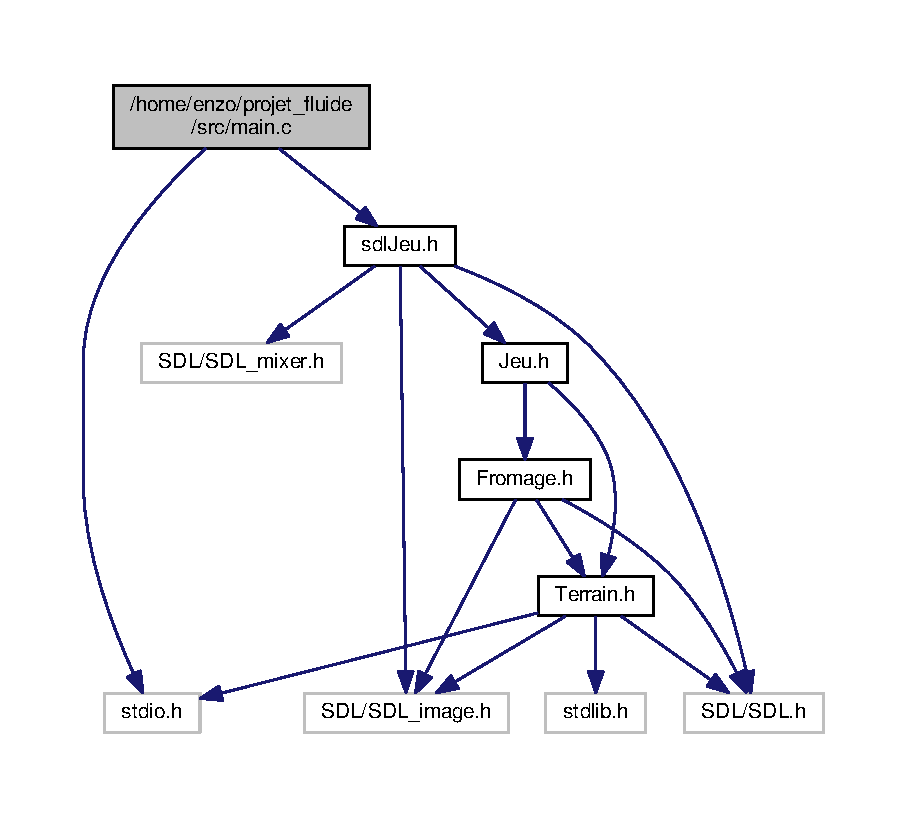
\includegraphics[width=350pt]{main_8c__incl}
\end{center}
\end{figure}
\subsection*{Macros}
\begin{DoxyCompactItemize}
\item 
\#define \hyperlink{main_8c_a7513cabb40cd35292dce4654b86160c8}{J\-E\-U\-\_\-\-S\-D\-L}
\end{DoxyCompactItemize}
\subsection*{Functions}
\begin{DoxyCompactItemize}
\item 
int \hyperlink{main_8c_a3c04138a5bfe5d72780bb7e82a18e627}{main} (int argc, char $\ast$$\ast$argv)
\end{DoxyCompactItemize}


\subsection{Macro Definition Documentation}
\hypertarget{main_8c_a7513cabb40cd35292dce4654b86160c8}{\index{main.\-c@{main.\-c}!J\-E\-U\-\_\-\-S\-D\-L@{J\-E\-U\-\_\-\-S\-D\-L}}
\index{J\-E\-U\-\_\-\-S\-D\-L@{J\-E\-U\-\_\-\-S\-D\-L}!main.c@{main.\-c}}
\subsubsection[{J\-E\-U\-\_\-\-S\-D\-L}]{\setlength{\rightskip}{0pt plus 5cm}\#define J\-E\-U\-\_\-\-S\-D\-L}}\label{main_8c_a7513cabb40cd35292dce4654b86160c8}


Definition at line 4 of file main.\-c.



\subsection{Function Documentation}
\hypertarget{main_8c_a3c04138a5bfe5d72780bb7e82a18e627}{\index{main.\-c@{main.\-c}!main@{main}}
\index{main@{main}!main.c@{main.\-c}}
\subsubsection[{main}]{\setlength{\rightskip}{0pt plus 5cm}int main (
\begin{DoxyParamCaption}
\item[{int}]{argc, }
\item[{char $\ast$$\ast$}]{argv}
\end{DoxyParamCaption}
)}}\label{main_8c_a3c04138a5bfe5d72780bb7e82a18e627}


Definition at line 15 of file main.\-c.



Here is the call graph for this function\-:
\nopagebreak
\begin{figure}[H]
\begin{center}
\leavevmode
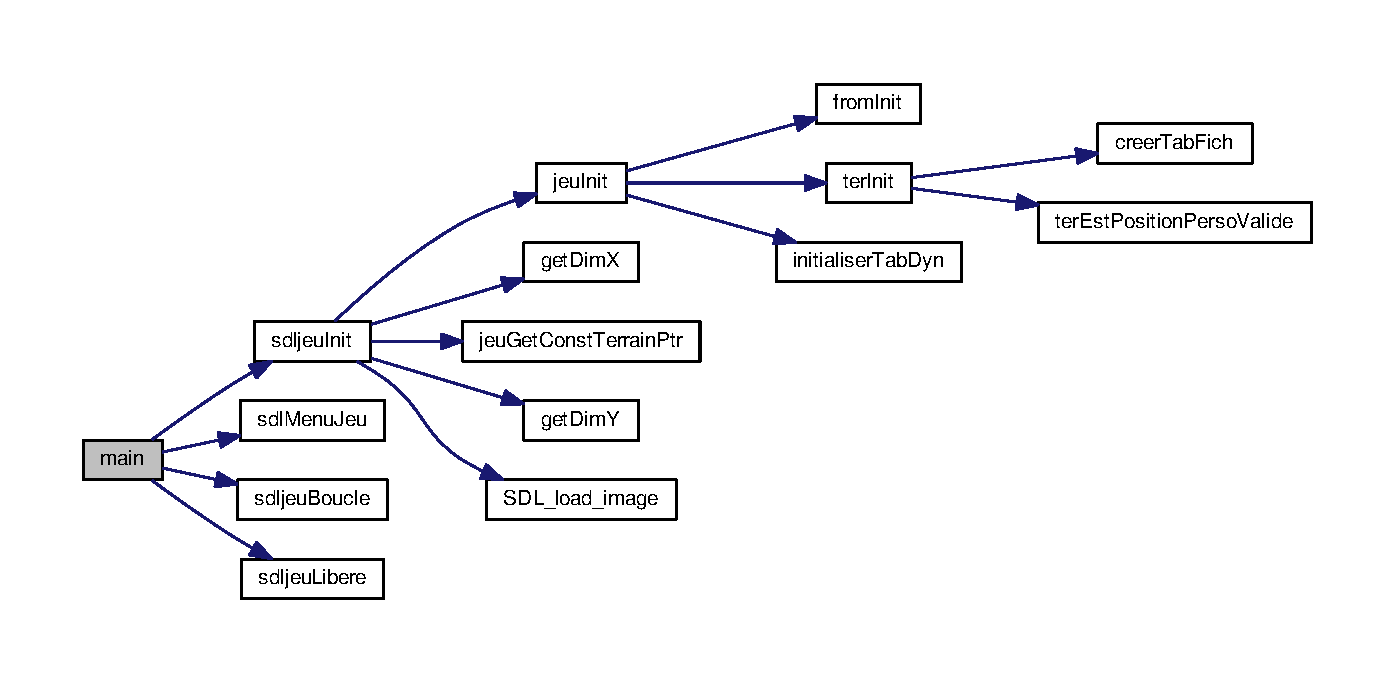
\includegraphics[width=350pt]{main_8c_a3c04138a5bfe5d72780bb7e82a18e627_cgraph}
\end{center}
\end{figure}



\hypertarget{menu_8c}{\section{/home/enzo/projet\-\_\-fluide/src/menu.c File Reference}
\label{menu_8c}\index{/home/enzo/projet\-\_\-fluide/src/menu.\-c@{/home/enzo/projet\-\_\-fluide/src/menu.\-c}}
}
{\ttfamily \#include $<$S\-D\-L/\-S\-D\-L.\-h$>$}\\*
{\ttfamily \#include $<$S\-D\-L/\-S\-D\-L\-\_\-image.\-h$>$}\\*
{\ttfamily \#include $<$stdio.\-h$>$}\\*
{\ttfamily \#include $<$stdlib.\-h$>$}\\*
Include dependency graph for menu.\-c\-:\nopagebreak
\begin{figure}[H]
\begin{center}
\leavevmode
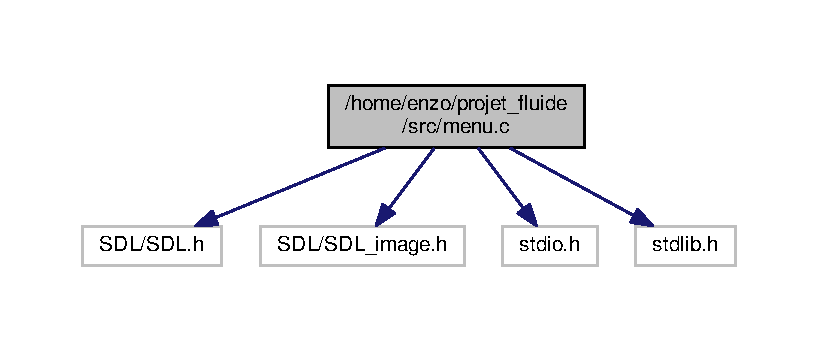
\includegraphics[width=350pt]{menu_8c__incl}
\end{center}
\end{figure}
\subsection*{Functions}
\begin{DoxyCompactItemize}
\item 
S\-D\-L\-\_\-\-Surface $\ast$ \hyperlink{menu_8c_aaf9c7736cab0f3cecd284f5fdb0b1683}{S\-D\-L\-\_\-load\-\_\-image} (const char $\ast$filename)
\item 
int \hyperlink{menu_8c_ae66f6b31b5ad750f1fe042a706a4e3d4}{main} ()
\end{DoxyCompactItemize}


\subsection{Function Documentation}
\hypertarget{menu_8c_ae66f6b31b5ad750f1fe042a706a4e3d4}{\index{menu.\-c@{menu.\-c}!main@{main}}
\index{main@{main}!menu.c@{menu.\-c}}
\subsubsection[{main}]{\setlength{\rightskip}{0pt plus 5cm}int main (
\begin{DoxyParamCaption}
{}
\end{DoxyParamCaption}
)}}\label{menu_8c_ae66f6b31b5ad750f1fe042a706a4e3d4}


Definition at line 31 of file menu.\-c.



Here is the call graph for this function\-:\nopagebreak
\begin{figure}[H]
\begin{center}
\leavevmode
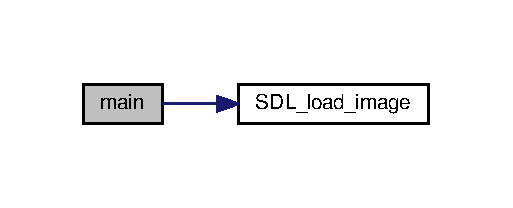
\includegraphics[width=246pt]{menu_8c_ae66f6b31b5ad750f1fe042a706a4e3d4_cgraph}
\end{center}
\end{figure}


\hypertarget{menu_8c_aaf9c7736cab0f3cecd284f5fdb0b1683}{\index{menu.\-c@{menu.\-c}!S\-D\-L\-\_\-load\-\_\-image@{S\-D\-L\-\_\-load\-\_\-image}}
\index{S\-D\-L\-\_\-load\-\_\-image@{S\-D\-L\-\_\-load\-\_\-image}!menu.c@{menu.\-c}}
\subsubsection[{S\-D\-L\-\_\-load\-\_\-image}]{\setlength{\rightskip}{0pt plus 5cm}S\-D\-L\-\_\-\-Surface$\ast$ S\-D\-L\-\_\-load\-\_\-image (
\begin{DoxyParamCaption}
\item[{const char $\ast$}]{filename}
\end{DoxyParamCaption}
)}}\label{menu_8c_aaf9c7736cab0f3cecd284f5fdb0b1683}


Definition at line 6 of file menu.\-c.


\hypertarget{sdl_jeu_8c}{\section{/home/enzo/projet\-\_\-fluide/src/sdl\-Jeu.c File Reference}
\label{sdl_jeu_8c}\index{/home/enzo/projet\-\_\-fluide/src/sdl\-Jeu.\-c@{/home/enzo/projet\-\_\-fluide/src/sdl\-Jeu.\-c}}
}
{\ttfamily \#include $<$assert.\-h$>$}\\*
{\ttfamily \#include $<$time.\-h$>$}\\*
{\ttfamily \#include \char`\"{}sdl\-Jeu.\-h\char`\"{}}\\*
Include dependency graph for sdl\-Jeu.\-c\-:\nopagebreak
\begin{figure}[H]
\begin{center}
\leavevmode
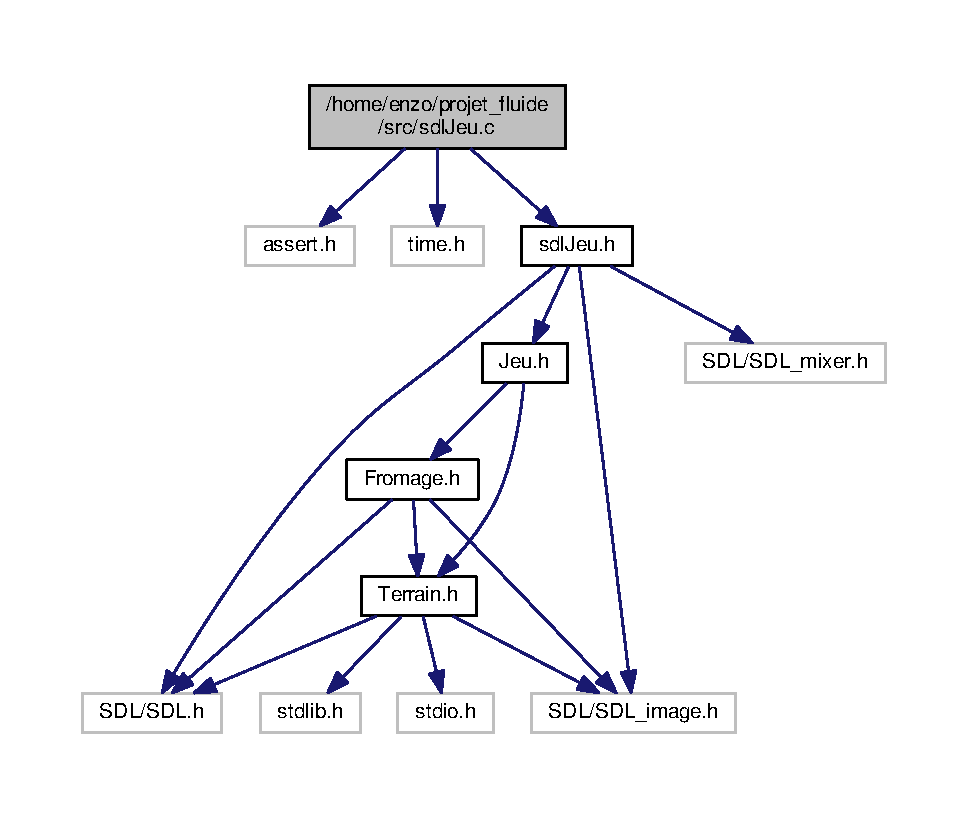
\includegraphics[width=350pt]{sdl_jeu_8c__incl}
\end{center}
\end{figure}
\subsection*{Macros}
\begin{DoxyCompactItemize}
\item 
\#define \hyperlink{sdl_jeu_8c_acd0f9b88c35112b35f67d3cde4b2365c}{H\-A\-U\-T}~0
\item 
\#define \hyperlink{sdl_jeu_8c_af625d3f3bc022848a558f2b18def5b15}{D\-R\-O\-I\-T\-E}~1
\item 
\#define \hyperlink{sdl_jeu_8c_abd7bcdd3b14eec4414469f88f2bd8f12}{B\-A\-S}~2
\item 
\#define \hyperlink{sdl_jeu_8c_af07f8bf974fdf76afd17f2b97ac15a22}{G\-A\-U\-C\-H\-E}~3
\item 
\#define \hyperlink{sdl_jeu_8c_a7dcae438e7824a23ed30d2139c1eff89}{A\-U\-C\-U\-N\-E\-\_\-\-D\-I\-R\-E\-C\-T\-I\-O\-N}~4
\item 
\#define \hyperlink{sdl_jeu_8c_a4104d8bac5f71c40e72de6aa5080e853}{D\-I\-R\-E\-C\-T\-I\-O\-N\-\_\-\-H\-A\-U\-T}~5
\item 
\#define \hyperlink{sdl_jeu_8c_a17b219a9666ba50f527efe5fecf9de4c}{D\-I\-R\-E\-C\-T\-I\-O\-N\-\_\-\-D\-R\-O\-I\-T\-E}~6
\item 
\#define \hyperlink{sdl_jeu_8c_a0439327d50e1021a81cff4d7dce7ac12}{D\-I\-R\-E\-C\-T\-I\-O\-N\-\_\-\-B\-A\-S}~7
\item 
\#define \hyperlink{sdl_jeu_8c_aab6eb63c11e2bab5f85e8488a3b30d5d}{D\-I\-R\-E\-C\-T\-I\-O\-N\-\_\-\-G\-A\-U\-C\-H\-E}~8
\item 
\#define \hyperlink{sdl_jeu_8c_a39bc6ce729110249c344aaff8ff6a0dc}{D\-I\-R\-E\-C\-T\-I\-O\-N\-\_\-\-D\-I\-A\-G\-\_\-\-D\-B}~9
\item 
\#define \hyperlink{sdl_jeu_8c_a76d11649f0994a3577d1a62424a40306}{D\-I\-R\-E\-C\-T\-I\-O\-N\-\_\-\-D\-I\-A\-G\-\_\-\-D\-H}~10
\item 
\#define \hyperlink{sdl_jeu_8c_a2d8442ac2899f514c940ed8cf5b74ae8}{D\-I\-R\-E\-C\-T\-I\-O\-N\-\_\-\-D\-I\-A\-G\-\_\-\-G\-B}~11
\item 
\#define \hyperlink{sdl_jeu_8c_a63fbf81f2bfe7ccd613b9a9d8e43352c}{D\-I\-R\-E\-C\-T\-I\-O\-N\-\_\-\-D\-I\-A\-G\-\_\-\-G\-H}~12
\item 
\#define \hyperlink{sdl_jeu_8c_a2484b01dd58573754311f24affa38005}{O\-R\-I\-E\-N\-T\-A\-T\-I\-O\-N\-\_\-\-D\-R\-O\-I\-T\-E}~13
\item 
\#define \hyperlink{sdl_jeu_8c_abd6253e86e781ad5fc9a74bf450bacc7}{O\-R\-I\-E\-N\-T\-A\-T\-I\-O\-N\-\_\-\-H\-A\-U\-T}~14
\item 
\#define \hyperlink{sdl_jeu_8c_a75f7acf2f21db3834069859b801c7e32}{O\-R\-I\-E\-N\-T\-A\-T\-I\-O\-N\-\_\-\-B\-A\-S}~15
\item 
\#define \hyperlink{sdl_jeu_8c_a2fa60451bc6ed1cefead0b514a40c674}{O\-R\-I\-E\-N\-T\-A\-T\-I\-O\-N\-\_\-\-G\-A\-U\-C\-H\-E}~16
\end{DoxyCompactItemize}
\subsection*{Functions}
\begin{DoxyCompactItemize}
\item 
S\-D\-L\-\_\-\-Surface $\ast$ \hyperlink{sdl_jeu_8c_aaf9c7736cab0f3cecd284f5fdb0b1683}{S\-D\-L\-\_\-load\-\_\-image} (const char $\ast$filename)
\item 
void \hyperlink{sdl_jeu_8c_a695e055ca801891bb79cc6f68ecbf2ae}{S\-D\-L\-\_\-apply\-\_\-surface} (S\-D\-L\-\_\-\-Surface $\ast$source, S\-D\-L\-\_\-\-Surface $\ast$destination, int x, int y)
\item 
void \hyperlink{sdl_jeu_8c_ae89d08c92730e6b1e20fabdccacd382b}{sdljeu\-Init} (\hyperlink{structsdl_jeu}{sdl\-Jeu} $\ast$p\-Sdl\-Jeu)
\begin{DoxyCompactList}\small\item\em sdljeu\-Init charge les image les sons ect \end{DoxyCompactList}\end{DoxyCompactItemize}
\subsection*{Variables}
\begin{DoxyCompactItemize}
\item 
const int \hyperlink{sdl_jeu_8c_a6c3723683dfe1e0731a0f01ebc2e84f9}{T\-A\-I\-L\-L\-E\-\_\-\-S\-P\-R\-I\-T\-E} =32
\end{DoxyCompactItemize}


\subsection{Macro Definition Documentation}
\hypertarget{sdl_jeu_8c_a7dcae438e7824a23ed30d2139c1eff89}{\index{sdl\-Jeu.\-c@{sdl\-Jeu.\-c}!A\-U\-C\-U\-N\-E\-\_\-\-D\-I\-R\-E\-C\-T\-I\-O\-N@{A\-U\-C\-U\-N\-E\-\_\-\-D\-I\-R\-E\-C\-T\-I\-O\-N}}
\index{A\-U\-C\-U\-N\-E\-\_\-\-D\-I\-R\-E\-C\-T\-I\-O\-N@{A\-U\-C\-U\-N\-E\-\_\-\-D\-I\-R\-E\-C\-T\-I\-O\-N}!sdlJeu.c@{sdl\-Jeu.\-c}}
\subsubsection[{A\-U\-C\-U\-N\-E\-\_\-\-D\-I\-R\-E\-C\-T\-I\-O\-N}]{\setlength{\rightskip}{0pt plus 5cm}\#define A\-U\-C\-U\-N\-E\-\_\-\-D\-I\-R\-E\-C\-T\-I\-O\-N~4}}\label{sdl_jeu_8c_a7dcae438e7824a23ed30d2139c1eff89}


Definition at line 10 of file sdl\-Jeu.\-c.

\hypertarget{sdl_jeu_8c_abd7bcdd3b14eec4414469f88f2bd8f12}{\index{sdl\-Jeu.\-c@{sdl\-Jeu.\-c}!B\-A\-S@{B\-A\-S}}
\index{B\-A\-S@{B\-A\-S}!sdlJeu.c@{sdl\-Jeu.\-c}}
\subsubsection[{B\-A\-S}]{\setlength{\rightskip}{0pt plus 5cm}\#define B\-A\-S~2}}\label{sdl_jeu_8c_abd7bcdd3b14eec4414469f88f2bd8f12}


Definition at line 7 of file sdl\-Jeu.\-c.

\hypertarget{sdl_jeu_8c_a0439327d50e1021a81cff4d7dce7ac12}{\index{sdl\-Jeu.\-c@{sdl\-Jeu.\-c}!D\-I\-R\-E\-C\-T\-I\-O\-N\-\_\-\-B\-A\-S@{D\-I\-R\-E\-C\-T\-I\-O\-N\-\_\-\-B\-A\-S}}
\index{D\-I\-R\-E\-C\-T\-I\-O\-N\-\_\-\-B\-A\-S@{D\-I\-R\-E\-C\-T\-I\-O\-N\-\_\-\-B\-A\-S}!sdlJeu.c@{sdl\-Jeu.\-c}}
\subsubsection[{D\-I\-R\-E\-C\-T\-I\-O\-N\-\_\-\-B\-A\-S}]{\setlength{\rightskip}{0pt plus 5cm}\#define D\-I\-R\-E\-C\-T\-I\-O\-N\-\_\-\-B\-A\-S~7}}\label{sdl_jeu_8c_a0439327d50e1021a81cff4d7dce7ac12}


Definition at line 13 of file sdl\-Jeu.\-c.

\hypertarget{sdl_jeu_8c_a39bc6ce729110249c344aaff8ff6a0dc}{\index{sdl\-Jeu.\-c@{sdl\-Jeu.\-c}!D\-I\-R\-E\-C\-T\-I\-O\-N\-\_\-\-D\-I\-A\-G\-\_\-\-D\-B@{D\-I\-R\-E\-C\-T\-I\-O\-N\-\_\-\-D\-I\-A\-G\-\_\-\-D\-B}}
\index{D\-I\-R\-E\-C\-T\-I\-O\-N\-\_\-\-D\-I\-A\-G\-\_\-\-D\-B@{D\-I\-R\-E\-C\-T\-I\-O\-N\-\_\-\-D\-I\-A\-G\-\_\-\-D\-B}!sdlJeu.c@{sdl\-Jeu.\-c}}
\subsubsection[{D\-I\-R\-E\-C\-T\-I\-O\-N\-\_\-\-D\-I\-A\-G\-\_\-\-D\-B}]{\setlength{\rightskip}{0pt plus 5cm}\#define D\-I\-R\-E\-C\-T\-I\-O\-N\-\_\-\-D\-I\-A\-G\-\_\-\-D\-B~9}}\label{sdl_jeu_8c_a39bc6ce729110249c344aaff8ff6a0dc}


Definition at line 15 of file sdl\-Jeu.\-c.

\hypertarget{sdl_jeu_8c_a76d11649f0994a3577d1a62424a40306}{\index{sdl\-Jeu.\-c@{sdl\-Jeu.\-c}!D\-I\-R\-E\-C\-T\-I\-O\-N\-\_\-\-D\-I\-A\-G\-\_\-\-D\-H@{D\-I\-R\-E\-C\-T\-I\-O\-N\-\_\-\-D\-I\-A\-G\-\_\-\-D\-H}}
\index{D\-I\-R\-E\-C\-T\-I\-O\-N\-\_\-\-D\-I\-A\-G\-\_\-\-D\-H@{D\-I\-R\-E\-C\-T\-I\-O\-N\-\_\-\-D\-I\-A\-G\-\_\-\-D\-H}!sdlJeu.c@{sdl\-Jeu.\-c}}
\subsubsection[{D\-I\-R\-E\-C\-T\-I\-O\-N\-\_\-\-D\-I\-A\-G\-\_\-\-D\-H}]{\setlength{\rightskip}{0pt plus 5cm}\#define D\-I\-R\-E\-C\-T\-I\-O\-N\-\_\-\-D\-I\-A\-G\-\_\-\-D\-H~10}}\label{sdl_jeu_8c_a76d11649f0994a3577d1a62424a40306}


Definition at line 16 of file sdl\-Jeu.\-c.

\hypertarget{sdl_jeu_8c_a2d8442ac2899f514c940ed8cf5b74ae8}{\index{sdl\-Jeu.\-c@{sdl\-Jeu.\-c}!D\-I\-R\-E\-C\-T\-I\-O\-N\-\_\-\-D\-I\-A\-G\-\_\-\-G\-B@{D\-I\-R\-E\-C\-T\-I\-O\-N\-\_\-\-D\-I\-A\-G\-\_\-\-G\-B}}
\index{D\-I\-R\-E\-C\-T\-I\-O\-N\-\_\-\-D\-I\-A\-G\-\_\-\-G\-B@{D\-I\-R\-E\-C\-T\-I\-O\-N\-\_\-\-D\-I\-A\-G\-\_\-\-G\-B}!sdlJeu.c@{sdl\-Jeu.\-c}}
\subsubsection[{D\-I\-R\-E\-C\-T\-I\-O\-N\-\_\-\-D\-I\-A\-G\-\_\-\-G\-B}]{\setlength{\rightskip}{0pt plus 5cm}\#define D\-I\-R\-E\-C\-T\-I\-O\-N\-\_\-\-D\-I\-A\-G\-\_\-\-G\-B~11}}\label{sdl_jeu_8c_a2d8442ac2899f514c940ed8cf5b74ae8}


Definition at line 17 of file sdl\-Jeu.\-c.

\hypertarget{sdl_jeu_8c_a63fbf81f2bfe7ccd613b9a9d8e43352c}{\index{sdl\-Jeu.\-c@{sdl\-Jeu.\-c}!D\-I\-R\-E\-C\-T\-I\-O\-N\-\_\-\-D\-I\-A\-G\-\_\-\-G\-H@{D\-I\-R\-E\-C\-T\-I\-O\-N\-\_\-\-D\-I\-A\-G\-\_\-\-G\-H}}
\index{D\-I\-R\-E\-C\-T\-I\-O\-N\-\_\-\-D\-I\-A\-G\-\_\-\-G\-H@{D\-I\-R\-E\-C\-T\-I\-O\-N\-\_\-\-D\-I\-A\-G\-\_\-\-G\-H}!sdlJeu.c@{sdl\-Jeu.\-c}}
\subsubsection[{D\-I\-R\-E\-C\-T\-I\-O\-N\-\_\-\-D\-I\-A\-G\-\_\-\-G\-H}]{\setlength{\rightskip}{0pt plus 5cm}\#define D\-I\-R\-E\-C\-T\-I\-O\-N\-\_\-\-D\-I\-A\-G\-\_\-\-G\-H~12}}\label{sdl_jeu_8c_a63fbf81f2bfe7ccd613b9a9d8e43352c}


Definition at line 18 of file sdl\-Jeu.\-c.

\hypertarget{sdl_jeu_8c_a17b219a9666ba50f527efe5fecf9de4c}{\index{sdl\-Jeu.\-c@{sdl\-Jeu.\-c}!D\-I\-R\-E\-C\-T\-I\-O\-N\-\_\-\-D\-R\-O\-I\-T\-E@{D\-I\-R\-E\-C\-T\-I\-O\-N\-\_\-\-D\-R\-O\-I\-T\-E}}
\index{D\-I\-R\-E\-C\-T\-I\-O\-N\-\_\-\-D\-R\-O\-I\-T\-E@{D\-I\-R\-E\-C\-T\-I\-O\-N\-\_\-\-D\-R\-O\-I\-T\-E}!sdlJeu.c@{sdl\-Jeu.\-c}}
\subsubsection[{D\-I\-R\-E\-C\-T\-I\-O\-N\-\_\-\-D\-R\-O\-I\-T\-E}]{\setlength{\rightskip}{0pt plus 5cm}\#define D\-I\-R\-E\-C\-T\-I\-O\-N\-\_\-\-D\-R\-O\-I\-T\-E~6}}\label{sdl_jeu_8c_a17b219a9666ba50f527efe5fecf9de4c}


Definition at line 12 of file sdl\-Jeu.\-c.

\hypertarget{sdl_jeu_8c_aab6eb63c11e2bab5f85e8488a3b30d5d}{\index{sdl\-Jeu.\-c@{sdl\-Jeu.\-c}!D\-I\-R\-E\-C\-T\-I\-O\-N\-\_\-\-G\-A\-U\-C\-H\-E@{D\-I\-R\-E\-C\-T\-I\-O\-N\-\_\-\-G\-A\-U\-C\-H\-E}}
\index{D\-I\-R\-E\-C\-T\-I\-O\-N\-\_\-\-G\-A\-U\-C\-H\-E@{D\-I\-R\-E\-C\-T\-I\-O\-N\-\_\-\-G\-A\-U\-C\-H\-E}!sdlJeu.c@{sdl\-Jeu.\-c}}
\subsubsection[{D\-I\-R\-E\-C\-T\-I\-O\-N\-\_\-\-G\-A\-U\-C\-H\-E}]{\setlength{\rightskip}{0pt plus 5cm}\#define D\-I\-R\-E\-C\-T\-I\-O\-N\-\_\-\-G\-A\-U\-C\-H\-E~8}}\label{sdl_jeu_8c_aab6eb63c11e2bab5f85e8488a3b30d5d}


Definition at line 14 of file sdl\-Jeu.\-c.

\hypertarget{sdl_jeu_8c_a4104d8bac5f71c40e72de6aa5080e853}{\index{sdl\-Jeu.\-c@{sdl\-Jeu.\-c}!D\-I\-R\-E\-C\-T\-I\-O\-N\-\_\-\-H\-A\-U\-T@{D\-I\-R\-E\-C\-T\-I\-O\-N\-\_\-\-H\-A\-U\-T}}
\index{D\-I\-R\-E\-C\-T\-I\-O\-N\-\_\-\-H\-A\-U\-T@{D\-I\-R\-E\-C\-T\-I\-O\-N\-\_\-\-H\-A\-U\-T}!sdlJeu.c@{sdl\-Jeu.\-c}}
\subsubsection[{D\-I\-R\-E\-C\-T\-I\-O\-N\-\_\-\-H\-A\-U\-T}]{\setlength{\rightskip}{0pt plus 5cm}\#define D\-I\-R\-E\-C\-T\-I\-O\-N\-\_\-\-H\-A\-U\-T~5}}\label{sdl_jeu_8c_a4104d8bac5f71c40e72de6aa5080e853}


Definition at line 11 of file sdl\-Jeu.\-c.

\hypertarget{sdl_jeu_8c_af625d3f3bc022848a558f2b18def5b15}{\index{sdl\-Jeu.\-c@{sdl\-Jeu.\-c}!D\-R\-O\-I\-T\-E@{D\-R\-O\-I\-T\-E}}
\index{D\-R\-O\-I\-T\-E@{D\-R\-O\-I\-T\-E}!sdlJeu.c@{sdl\-Jeu.\-c}}
\subsubsection[{D\-R\-O\-I\-T\-E}]{\setlength{\rightskip}{0pt plus 5cm}\#define D\-R\-O\-I\-T\-E~1}}\label{sdl_jeu_8c_af625d3f3bc022848a558f2b18def5b15}


Definition at line 6 of file sdl\-Jeu.\-c.

\hypertarget{sdl_jeu_8c_af07f8bf974fdf76afd17f2b97ac15a22}{\index{sdl\-Jeu.\-c@{sdl\-Jeu.\-c}!G\-A\-U\-C\-H\-E@{G\-A\-U\-C\-H\-E}}
\index{G\-A\-U\-C\-H\-E@{G\-A\-U\-C\-H\-E}!sdlJeu.c@{sdl\-Jeu.\-c}}
\subsubsection[{G\-A\-U\-C\-H\-E}]{\setlength{\rightskip}{0pt plus 5cm}\#define G\-A\-U\-C\-H\-E~3}}\label{sdl_jeu_8c_af07f8bf974fdf76afd17f2b97ac15a22}


Definition at line 8 of file sdl\-Jeu.\-c.

\hypertarget{sdl_jeu_8c_acd0f9b88c35112b35f67d3cde4b2365c}{\index{sdl\-Jeu.\-c@{sdl\-Jeu.\-c}!H\-A\-U\-T@{H\-A\-U\-T}}
\index{H\-A\-U\-T@{H\-A\-U\-T}!sdlJeu.c@{sdl\-Jeu.\-c}}
\subsubsection[{H\-A\-U\-T}]{\setlength{\rightskip}{0pt plus 5cm}\#define H\-A\-U\-T~0}}\label{sdl_jeu_8c_acd0f9b88c35112b35f67d3cde4b2365c}


Definition at line 5 of file sdl\-Jeu.\-c.

\hypertarget{sdl_jeu_8c_a75f7acf2f21db3834069859b801c7e32}{\index{sdl\-Jeu.\-c@{sdl\-Jeu.\-c}!O\-R\-I\-E\-N\-T\-A\-T\-I\-O\-N\-\_\-\-B\-A\-S@{O\-R\-I\-E\-N\-T\-A\-T\-I\-O\-N\-\_\-\-B\-A\-S}}
\index{O\-R\-I\-E\-N\-T\-A\-T\-I\-O\-N\-\_\-\-B\-A\-S@{O\-R\-I\-E\-N\-T\-A\-T\-I\-O\-N\-\_\-\-B\-A\-S}!sdlJeu.c@{sdl\-Jeu.\-c}}
\subsubsection[{O\-R\-I\-E\-N\-T\-A\-T\-I\-O\-N\-\_\-\-B\-A\-S}]{\setlength{\rightskip}{0pt plus 5cm}\#define O\-R\-I\-E\-N\-T\-A\-T\-I\-O\-N\-\_\-\-B\-A\-S~15}}\label{sdl_jeu_8c_a75f7acf2f21db3834069859b801c7e32}


Definition at line 21 of file sdl\-Jeu.\-c.

\hypertarget{sdl_jeu_8c_a2484b01dd58573754311f24affa38005}{\index{sdl\-Jeu.\-c@{sdl\-Jeu.\-c}!O\-R\-I\-E\-N\-T\-A\-T\-I\-O\-N\-\_\-\-D\-R\-O\-I\-T\-E@{O\-R\-I\-E\-N\-T\-A\-T\-I\-O\-N\-\_\-\-D\-R\-O\-I\-T\-E}}
\index{O\-R\-I\-E\-N\-T\-A\-T\-I\-O\-N\-\_\-\-D\-R\-O\-I\-T\-E@{O\-R\-I\-E\-N\-T\-A\-T\-I\-O\-N\-\_\-\-D\-R\-O\-I\-T\-E}!sdlJeu.c@{sdl\-Jeu.\-c}}
\subsubsection[{O\-R\-I\-E\-N\-T\-A\-T\-I\-O\-N\-\_\-\-D\-R\-O\-I\-T\-E}]{\setlength{\rightskip}{0pt plus 5cm}\#define O\-R\-I\-E\-N\-T\-A\-T\-I\-O\-N\-\_\-\-D\-R\-O\-I\-T\-E~13}}\label{sdl_jeu_8c_a2484b01dd58573754311f24affa38005}


Definition at line 19 of file sdl\-Jeu.\-c.

\hypertarget{sdl_jeu_8c_a2fa60451bc6ed1cefead0b514a40c674}{\index{sdl\-Jeu.\-c@{sdl\-Jeu.\-c}!O\-R\-I\-E\-N\-T\-A\-T\-I\-O\-N\-\_\-\-G\-A\-U\-C\-H\-E@{O\-R\-I\-E\-N\-T\-A\-T\-I\-O\-N\-\_\-\-G\-A\-U\-C\-H\-E}}
\index{O\-R\-I\-E\-N\-T\-A\-T\-I\-O\-N\-\_\-\-G\-A\-U\-C\-H\-E@{O\-R\-I\-E\-N\-T\-A\-T\-I\-O\-N\-\_\-\-G\-A\-U\-C\-H\-E}!sdlJeu.c@{sdl\-Jeu.\-c}}
\subsubsection[{O\-R\-I\-E\-N\-T\-A\-T\-I\-O\-N\-\_\-\-G\-A\-U\-C\-H\-E}]{\setlength{\rightskip}{0pt plus 5cm}\#define O\-R\-I\-E\-N\-T\-A\-T\-I\-O\-N\-\_\-\-G\-A\-U\-C\-H\-E~16}}\label{sdl_jeu_8c_a2fa60451bc6ed1cefead0b514a40c674}


Definition at line 22 of file sdl\-Jeu.\-c.

\hypertarget{sdl_jeu_8c_abd6253e86e781ad5fc9a74bf450bacc7}{\index{sdl\-Jeu.\-c@{sdl\-Jeu.\-c}!O\-R\-I\-E\-N\-T\-A\-T\-I\-O\-N\-\_\-\-H\-A\-U\-T@{O\-R\-I\-E\-N\-T\-A\-T\-I\-O\-N\-\_\-\-H\-A\-U\-T}}
\index{O\-R\-I\-E\-N\-T\-A\-T\-I\-O\-N\-\_\-\-H\-A\-U\-T@{O\-R\-I\-E\-N\-T\-A\-T\-I\-O\-N\-\_\-\-H\-A\-U\-T}!sdlJeu.c@{sdl\-Jeu.\-c}}
\subsubsection[{O\-R\-I\-E\-N\-T\-A\-T\-I\-O\-N\-\_\-\-H\-A\-U\-T}]{\setlength{\rightskip}{0pt plus 5cm}\#define O\-R\-I\-E\-N\-T\-A\-T\-I\-O\-N\-\_\-\-H\-A\-U\-T~14}}\label{sdl_jeu_8c_abd6253e86e781ad5fc9a74bf450bacc7}


Definition at line 20 of file sdl\-Jeu.\-c.



\subsection{Function Documentation}
\hypertarget{sdl_jeu_8c_a695e055ca801891bb79cc6f68ecbf2ae}{\index{sdl\-Jeu.\-c@{sdl\-Jeu.\-c}!S\-D\-L\-\_\-apply\-\_\-surface@{S\-D\-L\-\_\-apply\-\_\-surface}}
\index{S\-D\-L\-\_\-apply\-\_\-surface@{S\-D\-L\-\_\-apply\-\_\-surface}!sdlJeu.c@{sdl\-Jeu.\-c}}
\subsubsection[{S\-D\-L\-\_\-apply\-\_\-surface}]{\setlength{\rightskip}{0pt plus 5cm}void S\-D\-L\-\_\-apply\-\_\-surface (
\begin{DoxyParamCaption}
\item[{S\-D\-L\-\_\-\-Surface $\ast$}]{source, }
\item[{S\-D\-L\-\_\-\-Surface $\ast$}]{destination, }
\item[{int}]{x, }
\item[{int}]{y}
\end{DoxyParamCaption}
)}}\label{sdl_jeu_8c_a695e055ca801891bb79cc6f68ecbf2ae}
\hypertarget{sdl_jeu_8c_aaf9c7736cab0f3cecd284f5fdb0b1683}{\index{sdl\-Jeu.\-c@{sdl\-Jeu.\-c}!S\-D\-L\-\_\-load\-\_\-image@{S\-D\-L\-\_\-load\-\_\-image}}
\index{S\-D\-L\-\_\-load\-\_\-image@{S\-D\-L\-\_\-load\-\_\-image}!sdlJeu.c@{sdl\-Jeu.\-c}}
\subsubsection[{S\-D\-L\-\_\-load\-\_\-image}]{\setlength{\rightskip}{0pt plus 5cm}S\-D\-L\-\_\-\-Surface$\ast$ S\-D\-L\-\_\-load\-\_\-image (
\begin{DoxyParamCaption}
\item[{const char $\ast$}]{filename}
\end{DoxyParamCaption}
)}}\label{sdl_jeu_8c_aaf9c7736cab0f3cecd284f5fdb0b1683}


Definition at line 6 of file menu.\-c.

\hypertarget{sdl_jeu_8c_ae89d08c92730e6b1e20fabdccacd382b}{\index{sdl\-Jeu.\-c@{sdl\-Jeu.\-c}!sdljeu\-Init@{sdljeu\-Init}}
\index{sdljeu\-Init@{sdljeu\-Init}!sdlJeu.c@{sdl\-Jeu.\-c}}
\subsubsection[{sdljeu\-Init}]{\setlength{\rightskip}{0pt plus 5cm}void sdljeu\-Init (
\begin{DoxyParamCaption}
\item[{{\bf sdl\-Jeu} $\ast$}]{}
\end{DoxyParamCaption}
)}}\label{sdl_jeu_8c_ae89d08c92730e6b1e20fabdccacd382b}


sdljeu\-Init charge les image les sons ect 


\begin{DoxyParams}{Parameters}
{\em sdl\-Jeu$\ast$} & \\
\hline
\end{DoxyParams}


Definition at line 29 of file sdl\-Jeu.\-c.



Here is the call graph for this function\-:
\nopagebreak
\begin{figure}[H]
\begin{center}
\leavevmode
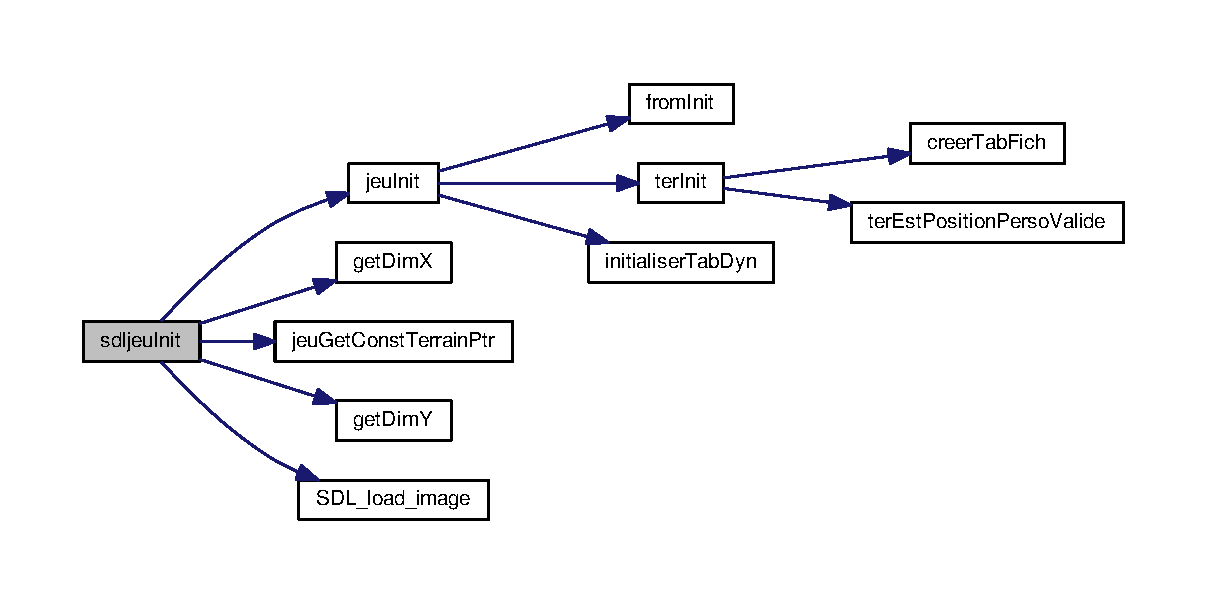
\includegraphics[width=350pt]{sdl_jeu_8c_ae89d08c92730e6b1e20fabdccacd382b_cgraph}
\end{center}
\end{figure}




\subsection{Variable Documentation}
\hypertarget{sdl_jeu_8c_a6c3723683dfe1e0731a0f01ebc2e84f9}{\index{sdl\-Jeu.\-c@{sdl\-Jeu.\-c}!T\-A\-I\-L\-L\-E\-\_\-\-S\-P\-R\-I\-T\-E@{T\-A\-I\-L\-L\-E\-\_\-\-S\-P\-R\-I\-T\-E}}
\index{T\-A\-I\-L\-L\-E\-\_\-\-S\-P\-R\-I\-T\-E@{T\-A\-I\-L\-L\-E\-\_\-\-S\-P\-R\-I\-T\-E}!sdlJeu.c@{sdl\-Jeu.\-c}}
\subsubsection[{T\-A\-I\-L\-L\-E\-\_\-\-S\-P\-R\-I\-T\-E}]{\setlength{\rightskip}{0pt plus 5cm}const int T\-A\-I\-L\-L\-E\-\_\-\-S\-P\-R\-I\-T\-E =32}}\label{sdl_jeu_8c_a6c3723683dfe1e0731a0f01ebc2e84f9}


Definition at line 24 of file sdl\-Jeu.\-c.


\hypertarget{sdl_jeu_8h}{\section{/home/enzo/projet\-\_\-fluide/src/sdl\-Jeu.h File Reference}
\label{sdl_jeu_8h}\index{/home/enzo/projet\-\_\-fluide/src/sdl\-Jeu.\-h@{/home/enzo/projet\-\_\-fluide/src/sdl\-Jeu.\-h}}
}
{\ttfamily \#include $<$S\-D\-L/\-S\-D\-L.\-h$>$}\\*
{\ttfamily \#include $<$S\-D\-L/\-S\-D\-L\-\_\-image.\-h$>$}\\*
{\ttfamily \#include $<$S\-D\-L/\-S\-D\-L\-\_\-mixer.\-h$>$}\\*
{\ttfamily \#include \char`\"{}Jeu.\-h\char`\"{}}\\*
Include dependency graph for sdl\-Jeu.\-h\-:\nopagebreak
\begin{figure}[H]
\begin{center}
\leavevmode
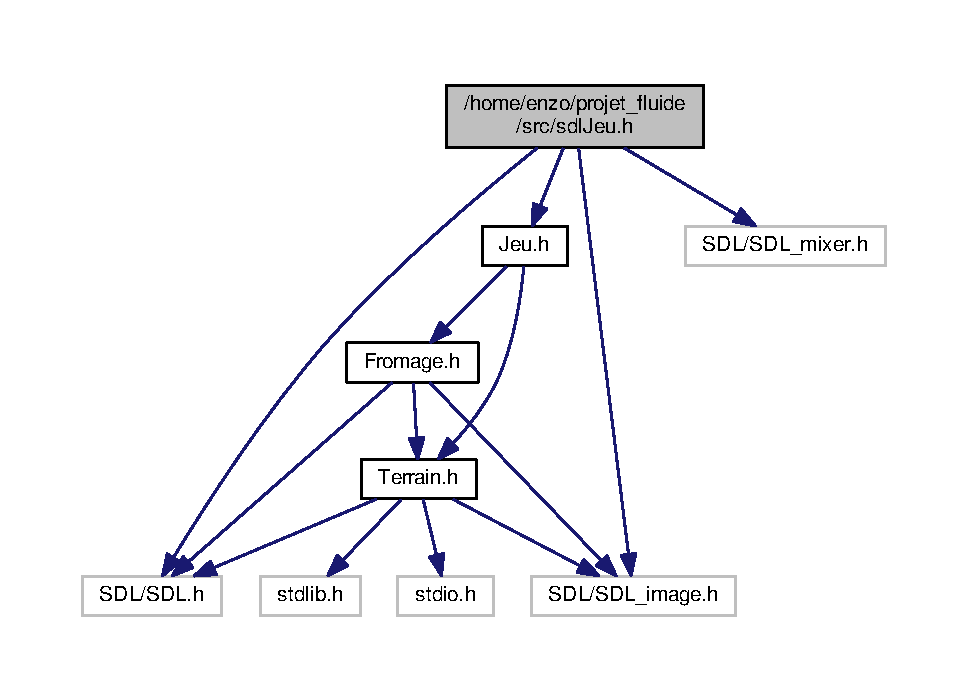
\includegraphics[width=350pt]{sdl_jeu_8h__incl}
\end{center}
\end{figure}
This graph shows which files directly or indirectly include this file\-:
\nopagebreak
\begin{figure}[H]
\begin{center}
\leavevmode
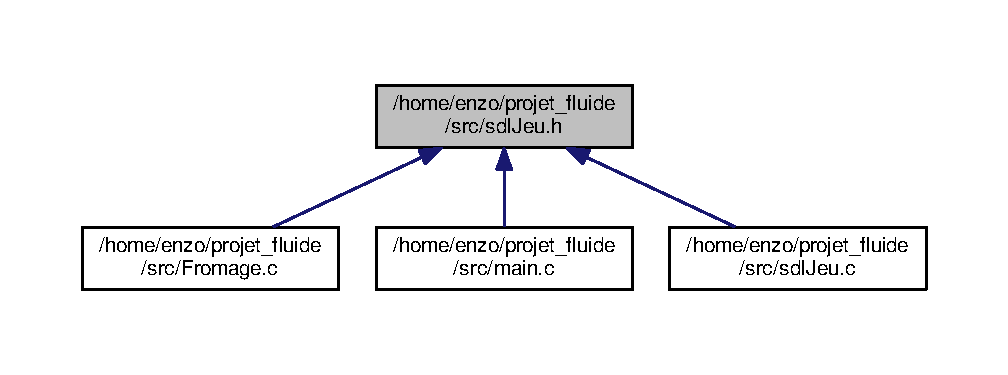
\includegraphics[width=350pt]{sdl_jeu_8h__dep__incl}
\end{center}
\end{figure}
\subsection*{Data Structures}
\begin{DoxyCompactItemize}
\item 
struct \hyperlink{struct_input}{Input}
\item 
struct \hyperlink{structsdl_jeu}{sdl\-Jeu}
\end{DoxyCompactItemize}
\subsection*{Functions}
\begin{DoxyCompactItemize}
\item 
void \hyperlink{sdl_jeu_8h_a1f8c7ab03690259e3bfd531029efb8c0}{sdljeu\-Init} (\hyperlink{structsdl_jeu}{sdl\-Jeu} $\ast$)
\begin{DoxyCompactList}\small\item\em sdljeu\-Init charge les image les sons ect \end{DoxyCompactList}\item 
void \hyperlink{sdl_jeu_8h_a08ca24693a92b1e137193664cf887c25}{sdl\-Menu\-Jeu} (\hyperlink{structsdl_jeu}{sdl\-Jeu} $\ast$)
\begin{DoxyCompactList}\small\item\em sdl\-Menu\-Jeu affiche le menu \end{DoxyCompactList}\item 
void \hyperlink{sdl_jeu_8h_a96254bfd4986200aa20f4781cdd7eb69}{sdljeu\-Boucle} (\hyperlink{structsdl_jeu}{sdl\-Jeu} $\ast$)
\begin{DoxyCompactList}\small\item\em sdljeu\-Boucle attend des actions du joueur, appel jeu\-Evolue, appel la fin du jeu... \end{DoxyCompactList}\item 
void \hyperlink{sdl_jeu_8h_a13daf0f06225b24df6ae754090ccd0f6}{sdljeu\-Libere} (\hyperlink{structsdl_jeu}{sdl\-Jeu} $\ast$)
\begin{DoxyCompactList}\small\item\em Libere toutes les fonctions du jeu. \end{DoxyCompactList}\end{DoxyCompactItemize}


\subsection{Function Documentation}
\hypertarget{sdl_jeu_8h_a96254bfd4986200aa20f4781cdd7eb69}{\index{sdl\-Jeu.\-h@{sdl\-Jeu.\-h}!sdljeu\-Boucle@{sdljeu\-Boucle}}
\index{sdljeu\-Boucle@{sdljeu\-Boucle}!sdlJeu.h@{sdl\-Jeu.\-h}}
\subsubsection[{sdljeu\-Boucle}]{\setlength{\rightskip}{0pt plus 5cm}void sdljeu\-Boucle (
\begin{DoxyParamCaption}
\item[{{\bf sdl\-Jeu} $\ast$}]{}
\end{DoxyParamCaption}
)}}\label{sdl_jeu_8h_a96254bfd4986200aa20f4781cdd7eb69}


sdljeu\-Boucle attend des actions du joueur, appel jeu\-Evolue, appel la fin du jeu... 


\begin{DoxyParams}{Parameters}
{\em \hyperlink{structsdl_jeu}{sdl\-Jeu}} & $\ast$ \\
\hline
\end{DoxyParams}
\hypertarget{sdl_jeu_8h_a1f8c7ab03690259e3bfd531029efb8c0}{\index{sdl\-Jeu.\-h@{sdl\-Jeu.\-h}!sdljeu\-Init@{sdljeu\-Init}}
\index{sdljeu\-Init@{sdljeu\-Init}!sdlJeu.h@{sdl\-Jeu.\-h}}
\subsubsection[{sdljeu\-Init}]{\setlength{\rightskip}{0pt plus 5cm}void sdljeu\-Init (
\begin{DoxyParamCaption}
\item[{{\bf sdl\-Jeu} $\ast$}]{}
\end{DoxyParamCaption}
)}}\label{sdl_jeu_8h_a1f8c7ab03690259e3bfd531029efb8c0}


sdljeu\-Init charge les image les sons ect 


\begin{DoxyParams}{Parameters}
{\em sdl\-Jeu$\ast$} & \\
\hline
\end{DoxyParams}


Definition at line 29 of file sdl\-Jeu.\-c.



Here is the call graph for this function\-:
\nopagebreak
\begin{figure}[H]
\begin{center}
\leavevmode
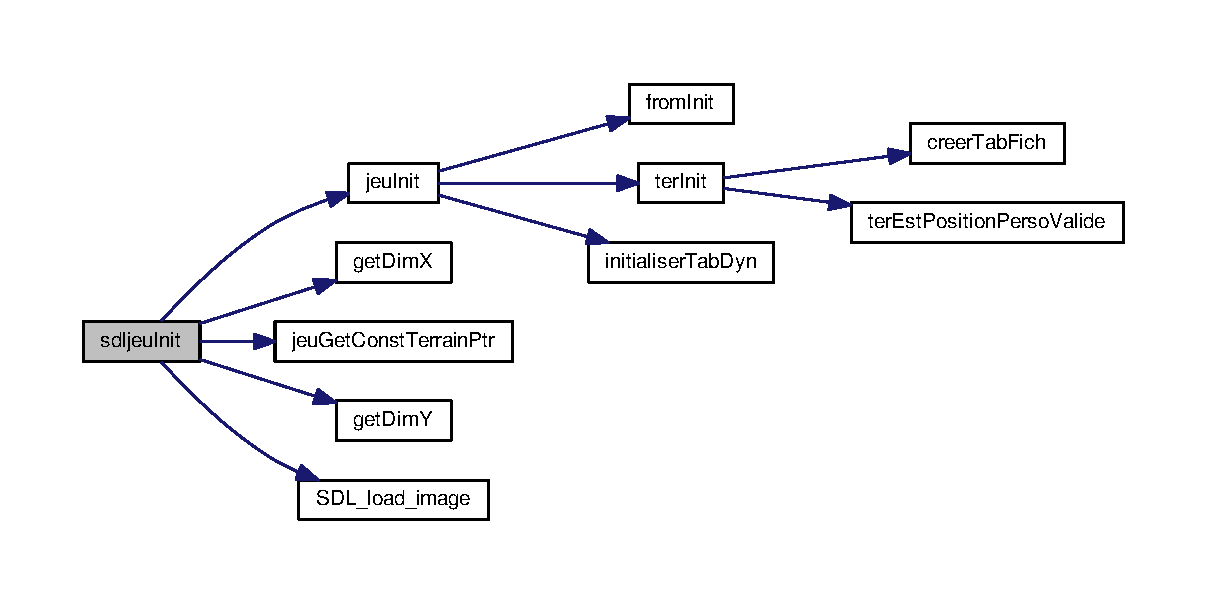
\includegraphics[width=350pt]{sdl_jeu_8h_a1f8c7ab03690259e3bfd531029efb8c0_cgraph}
\end{center}
\end{figure}


\hypertarget{sdl_jeu_8h_a13daf0f06225b24df6ae754090ccd0f6}{\index{sdl\-Jeu.\-h@{sdl\-Jeu.\-h}!sdljeu\-Libere@{sdljeu\-Libere}}
\index{sdljeu\-Libere@{sdljeu\-Libere}!sdlJeu.h@{sdl\-Jeu.\-h}}
\subsubsection[{sdljeu\-Libere}]{\setlength{\rightskip}{0pt plus 5cm}void sdljeu\-Libere (
\begin{DoxyParamCaption}
\item[{{\bf sdl\-Jeu} $\ast$}]{}
\end{DoxyParamCaption}
)}}\label{sdl_jeu_8h_a13daf0f06225b24df6ae754090ccd0f6}


Libere toutes les fonctions du jeu. 


\begin{DoxyParams}{Parameters}
{\em sdl\-Jeu$\ast$} & \\
\hline
\end{DoxyParams}
\hypertarget{sdl_jeu_8h_a08ca24693a92b1e137193664cf887c25}{\index{sdl\-Jeu.\-h@{sdl\-Jeu.\-h}!sdl\-Menu\-Jeu@{sdl\-Menu\-Jeu}}
\index{sdl\-Menu\-Jeu@{sdl\-Menu\-Jeu}!sdlJeu.h@{sdl\-Jeu.\-h}}
\subsubsection[{sdl\-Menu\-Jeu}]{\setlength{\rightskip}{0pt plus 5cm}void sdl\-Menu\-Jeu (
\begin{DoxyParamCaption}
\item[{{\bf sdl\-Jeu} $\ast$}]{}
\end{DoxyParamCaption}
)}}\label{sdl_jeu_8h_a08ca24693a92b1e137193664cf887c25}


sdl\-Menu\-Jeu affiche le menu 


\begin{DoxyParams}{Parameters}
{\em \hyperlink{structsdl_jeu}{sdl\-Jeu}} & $\ast$ \\
\hline
\end{DoxyParams}

\hypertarget{_terrain_8c}{\section{/home/enzo/projet\-\_\-fluide/src/\-Terrain.c File Reference}
\label{_terrain_8c}\index{/home/enzo/projet\-\_\-fluide/src/\-Terrain.\-c@{/home/enzo/projet\-\_\-fluide/src/\-Terrain.\-c}}
}
{\ttfamily \#include \char`\"{}Terrain.\-h\char`\"{}}\\*
{\ttfamily \#include $<$malloc.\-h$>$}\\*
{\ttfamily \#include $<$assert.\-h$>$}\\*
Include dependency graph for Terrain.\-c\-:\nopagebreak
\begin{figure}[H]
\begin{center}
\leavevmode
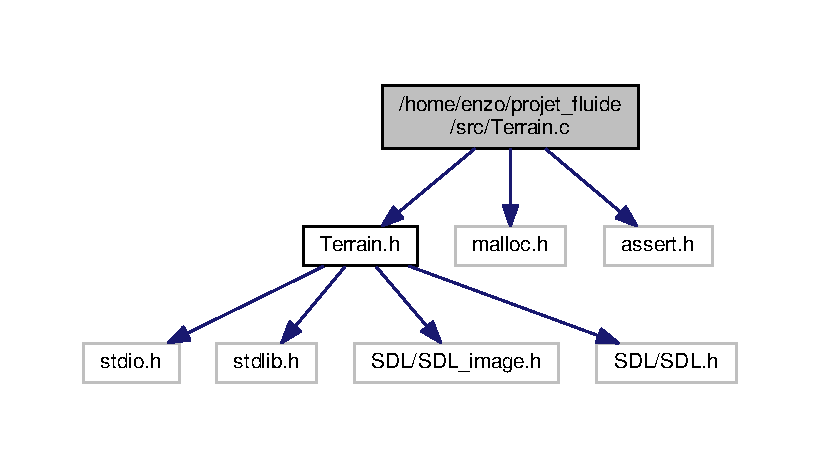
\includegraphics[width=350pt]{_terrain_8c__incl}
\end{center}
\end{figure}
\subsection*{Functions}
\begin{DoxyCompactItemize}
\item 
void \hyperlink{_terrain_8c_a44312d3c7ca6ef4573d206043149fc1f}{ter\-Init} (\hyperlink{struct_terrain}{Terrain} $\ast$p\-Niv)
\begin{DoxyCompactList}\small\item\em ter\-Init initialise le terrain \end{DoxyCompactList}\item 
void \hyperlink{_terrain_8c_a33518ef49d0daf247e25dcba54cda262}{init\-Fant} (\hyperlink{struct_terrain}{Terrain} $\ast$p\-Niv)
\begin{DoxyCompactList}\small\item\em init\-Fant initialise les ennemis \end{DoxyCompactList}\item 
void \hyperlink{_terrain_8c_a14e0a3176d0d5ddb34f2b1952918f147}{ter\-Actuel\-Initdroite} (\hyperlink{struct_terrain}{Terrain} $\ast$p\-Niv)
\begin{DoxyCompactList}\small\item\em ter\-Actuel\-Initdroite actualise le terrain si le personage est passe pas la porte de droite \end{DoxyCompactList}\item 
void \hyperlink{_terrain_8c_a1e312df917899f9253e9c17c4a7a27b4}{ter\-Actuel\-Initgauche} (\hyperlink{struct_terrain}{Terrain} $\ast$p\-Niv)
\begin{DoxyCompactList}\small\item\em ter\-Actuel\-Initdroite actualise le terrain si le personage est passe pas la porte de gauche \end{DoxyCompactList}\item 
void \hyperlink{_terrain_8c_afe8af29397b0175d7f76734389d78e22}{ter\-Actuel\-Inithaut} (\hyperlink{struct_terrain}{Terrain} $\ast$p\-Niv)
\begin{DoxyCompactList}\small\item\em ter\-Actuel\-Initdroite actualise le terrain si le personage est passe pas la porte de haut \end{DoxyCompactList}\item 
void \hyperlink{_terrain_8c_a2e6569ac0adacadee9d801af23836e83}{ter\-Actuel\-Initbas} (\hyperlink{struct_terrain}{Terrain} $\ast$p\-Niv)
\begin{DoxyCompactList}\small\item\em ter\-Actuel\-Initdroite actualise le terrain si le personage est passe pas la porte de bas \end{DoxyCompactList}\item 
void \hyperlink{_terrain_8c_aa8121b2fc06d3aa777c8303f0f36317d}{creer\-Tab\-Fich} (\hyperlink{struct_terrain}{Terrain} $\ast$t)
\item 
void \hyperlink{_terrain_8c_ac4ec9eb0a375fb3b0d9da191f4af5809}{ter\-Libere} (\hyperlink{struct_terrain}{Terrain} $\ast$p\-Niv)
\begin{DoxyCompactList}\small\item\em libere le terrain \end{DoxyCompactList}\item 
void \hyperlink{_terrain_8c_a65f656bd303453c5fadac03ae22ec70b}{vider} (\hyperlink{_terrain_8h_a00ea6820934a8f863026cfbfad337db8}{Salle} $\ast$n)
\item 
int \hyperlink{_terrain_8c_a5a60ae0eec54d0765a5c50a5e91181d5}{ter\-Est\-Position\-Perso\-Valide} (const \hyperlink{struct_terrain}{Terrain} $\ast$p\-Ter, const int x, const int y)
\begin{DoxyCompactList}\small\item\em ter\-Est\-Pos\-Perso\-Valide regarde si la position d'une entite est conforme au décors \end{DoxyCompactList}\item 
int \hyperlink{_terrain_8c_ad1b490ea518a26c59fb14b0c5a2321da}{ter\-Est\-Position\-Perso\-Pic} (const \hyperlink{struct_terrain}{Terrain} $\ast$p\-Ter, const int x, const int y)
\begin{DoxyCompactList}\small\item\em regarde si le personnage marche sur un pique \end{DoxyCompactList}\item 
int \hyperlink{_terrain_8c_abdecbecd10a7d628f4633ccde91dd9b0}{ter\-Est\-Position\-Perso\-Valide\-Pix} (const \hyperlink{struct_terrain}{Terrain} $\ast$p\-Ter, const int x, const int y)
\item 
void \hyperlink{_terrain_8c_a39cd3543cb66f7e189f348be4f891341}{perso\-Proche\-Rat} (const \hyperlink{struct_terrain}{Terrain} $\ast$p\-Ter, const int x, const int y)
\begin{DoxyCompactList}\small\item\em regarde si le personnage est proche des ennemis \end{DoxyCompactList}\item 
int \hyperlink{_terrain_8c_a0d53c6f5be499e7c90d722655a2f16ca}{pos\-Rat} (const \hyperlink{struct_terrain}{Terrain} $\ast$p\-Ter, int num\-\_\-rat)
\item 
void \hyperlink{_terrain_8c_a0a181b4a1f931a0df0306e6a6532790f}{mode\-Agro} (const \hyperlink{struct_terrain}{Terrain} $\ast$p\-Ter, const int x, const int y, const int i\-\_\-fant)
\begin{DoxyCompactList}\small\item\em fait en sorte que les ennemis attaquent le personnage \end{DoxyCompactList}\item 
int \hyperlink{_terrain_8c_ae1b854629b4514b6e4a4807a0e64f216}{Marqueur\-Present} (const \hyperlink{struct_terrain}{Terrain} $\ast$p\-Ter, const int x, const int y)
\begin{DoxyCompactList}\small\item\em Marqueur\-Present regarde si il y a un marqueur dans une case precise du tableau si oui, les enemis ne pas peuvent passer. \end{DoxyCompactList}\item 
const char \hyperlink{_terrain_8c_a43e155974fd55979d4eca34f5025bb43}{ter\-Get\-X\-Y} (const \hyperlink{struct_terrain}{Terrain} $\ast$p\-Ter, const int x, const int y)
\begin{DoxyCompactList}\small\item\em donne le contenu de la case xy \end{DoxyCompactList}\item 
void \hyperlink{_terrain_8c_a0a32fa4c6166a41d024da8e499fab0cb}{ter\-Set\-X\-Y} (const \hyperlink{struct_terrain}{Terrain} $\ast$p\-Ter, const int x, const int y, const char val)
\begin{DoxyCompactList}\small\item\em change le contenu de la case xy \end{DoxyCompactList}\item 
const int \hyperlink{_terrain_8c_a894e796af5dd61fa8e8879d74c4c197b}{get\-Dim\-X} (const \hyperlink{struct_terrain}{Terrain} $\ast$p\-Ter)
\begin{DoxyCompactList}\small\item\em donne la taille du terrain \end{DoxyCompactList}\item 
const int \hyperlink{_terrain_8c_af3b892a93ee78d81a03111d8b00231fe}{get\-Dim\-Y} (const \hyperlink{struct_terrain}{Terrain} $\ast$p\-Ter)
\begin{DoxyCompactList}\small\item\em donne la taille du terrain \end{DoxyCompactList}\item 
const int \hyperlink{_terrain_8c_ac3fec7537c44d9f2ed607a0d0b0f7e59}{getnbfant} (const \hyperlink{struct_terrain}{Terrain} $\ast$p\-Ter)
\begin{DoxyCompactList}\small\item\em regarde le nombre d'ennemis dans une salle \end{DoxyCompactList}\end{DoxyCompactItemize}


\subsection{Function Documentation}
\hypertarget{_terrain_8c_aa8121b2fc06d3aa777c8303f0f36317d}{\index{Terrain.\-c@{Terrain.\-c}!creer\-Tab\-Fich@{creer\-Tab\-Fich}}
\index{creer\-Tab\-Fich@{creer\-Tab\-Fich}!Terrain.c@{Terrain.\-c}}
\subsubsection[{creer\-Tab\-Fich}]{\setlength{\rightskip}{0pt plus 5cm}void creer\-Tab\-Fich (
\begin{DoxyParamCaption}
\item[{{\bf Terrain} $\ast$}]{t}
\end{DoxyParamCaption}
)}}\label{_terrain_8c_aa8121b2fc06d3aa777c8303f0f36317d}


Definition at line 410 of file Terrain.\-c.

\hypertarget{_terrain_8c_a894e796af5dd61fa8e8879d74c4c197b}{\index{Terrain.\-c@{Terrain.\-c}!get\-Dim\-X@{get\-Dim\-X}}
\index{get\-Dim\-X@{get\-Dim\-X}!Terrain.c@{Terrain.\-c}}
\subsubsection[{get\-Dim\-X}]{\setlength{\rightskip}{0pt plus 5cm}const int get\-Dim\-X (
\begin{DoxyParamCaption}
\item[{const {\bf Terrain} $\ast$}]{}
\end{DoxyParamCaption}
)}}\label{_terrain_8c_a894e796af5dd61fa8e8879d74c4c197b}


donne la taille du terrain 


\begin{DoxyParams}{Parameters}
{\em \hyperlink{struct_terrain}{Terrain}} & $\ast$ \\
\hline
\end{DoxyParams}


Definition at line 545 of file Terrain.\-c.

\hypertarget{_terrain_8c_af3b892a93ee78d81a03111d8b00231fe}{\index{Terrain.\-c@{Terrain.\-c}!get\-Dim\-Y@{get\-Dim\-Y}}
\index{get\-Dim\-Y@{get\-Dim\-Y}!Terrain.c@{Terrain.\-c}}
\subsubsection[{get\-Dim\-Y}]{\setlength{\rightskip}{0pt plus 5cm}const int get\-Dim\-Y (
\begin{DoxyParamCaption}
\item[{const {\bf Terrain} $\ast$}]{}
\end{DoxyParamCaption}
)}}\label{_terrain_8c_af3b892a93ee78d81a03111d8b00231fe}


donne la taille du terrain 


\begin{DoxyParams}{Parameters}
{\em \hyperlink{struct_terrain}{Terrain}} & $\ast$ \\
\hline
\end{DoxyParams}


Definition at line 550 of file Terrain.\-c.

\hypertarget{_terrain_8c_ac3fec7537c44d9f2ed607a0d0b0f7e59}{\index{Terrain.\-c@{Terrain.\-c}!getnbfant@{getnbfant}}
\index{getnbfant@{getnbfant}!Terrain.c@{Terrain.\-c}}
\subsubsection[{getnbfant}]{\setlength{\rightskip}{0pt plus 5cm}const int getnbfant (
\begin{DoxyParamCaption}
\item[{const {\bf Terrain} $\ast$}]{}
\end{DoxyParamCaption}
)}}\label{_terrain_8c_ac3fec7537c44d9f2ed607a0d0b0f7e59}


regarde le nombre d'ennemis dans une salle 


\begin{DoxyParams}{Parameters}
{\em \hyperlink{struct_terrain}{Terrain}} & $\ast$ \\
\hline
\end{DoxyParams}


Definition at line 555 of file Terrain.\-c.

\hypertarget{_terrain_8c_a33518ef49d0daf247e25dcba54cda262}{\index{Terrain.\-c@{Terrain.\-c}!init\-Fant@{init\-Fant}}
\index{init\-Fant@{init\-Fant}!Terrain.c@{Terrain.\-c}}
\subsubsection[{init\-Fant}]{\setlength{\rightskip}{0pt plus 5cm}void init\-Fant (
\begin{DoxyParamCaption}
\item[{{\bf Terrain} $\ast$}]{}
\end{DoxyParamCaption}
)}}\label{_terrain_8c_a33518ef49d0daf247e25dcba54cda262}


init\-Fant initialise les ennemis 


\begin{DoxyParams}{Parameters}
{\em \hyperlink{struct_terrain}{Terrain}} & $\ast$ \\
\hline
\end{DoxyParams}


Definition at line 310 of file Terrain.\-c.



Here is the call graph for this function\-:\nopagebreak
\begin{figure}[H]
\begin{center}
\leavevmode
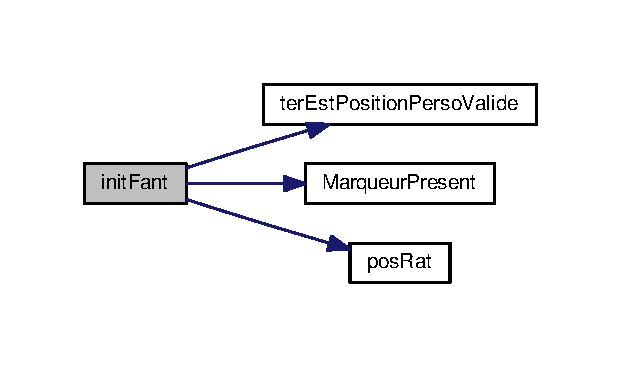
\includegraphics[width=298pt]{_terrain_8c_a33518ef49d0daf247e25dcba54cda262_cgraph}
\end{center}
\end{figure}


\hypertarget{_terrain_8c_ae1b854629b4514b6e4a4807a0e64f216}{\index{Terrain.\-c@{Terrain.\-c}!Marqueur\-Present@{Marqueur\-Present}}
\index{Marqueur\-Present@{Marqueur\-Present}!Terrain.c@{Terrain.\-c}}
\subsubsection[{Marqueur\-Present}]{\setlength{\rightskip}{0pt plus 5cm}int Marqueur\-Present (
\begin{DoxyParamCaption}
\item[{const {\bf Terrain} $\ast$}]{, }
\item[{const int}]{, }
\item[{const int}]{}
\end{DoxyParamCaption}
)}}\label{_terrain_8c_ae1b854629b4514b6e4a4807a0e64f216}


Marqueur\-Present regarde si il y a un marqueur dans une case precise du tableau si oui, les enemis ne pas peuvent passer. 


\begin{DoxyParams}{Parameters}
{\em \hyperlink{struct_terrain}{Terrain}} & $\ast$ \\
\hline
{\em int} & \\
\hline
{\em int} & \\
\hline
\end{DoxyParams}


Definition at line 511 of file Terrain.\-c.

\hypertarget{_terrain_8c_a0a181b4a1f931a0df0306e6a6532790f}{\index{Terrain.\-c@{Terrain.\-c}!mode\-Agro@{mode\-Agro}}
\index{mode\-Agro@{mode\-Agro}!Terrain.c@{Terrain.\-c}}
\subsubsection[{mode\-Agro}]{\setlength{\rightskip}{0pt plus 5cm}void mode\-Agro (
\begin{DoxyParamCaption}
\item[{const {\bf Terrain} $\ast$}]{, }
\item[{const int}]{, }
\item[{const int}]{, }
\item[{const int}]{}
\end{DoxyParamCaption}
)}}\label{_terrain_8c_a0a181b4a1f931a0df0306e6a6532790f}


fait en sorte que les ennemis attaquent le personnage 


\begin{DoxyParams}{Parameters}
{\em \hyperlink{struct_terrain}{Terrain}} & $\ast$ \\
\hline
{\em int} & \\
\hline
{\em int} & \\
\hline
{\em int} & \\
\hline
\end{DoxyParams}


Definition at line 486 of file Terrain.\-c.



Here is the call graph for this function\-:\nopagebreak
\begin{figure}[H]
\begin{center}
\leavevmode
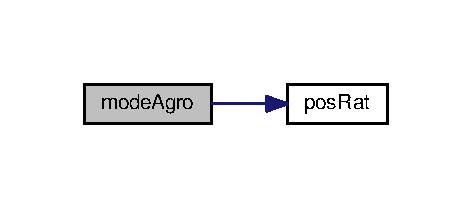
\includegraphics[width=226pt]{_terrain_8c_a0a181b4a1f931a0df0306e6a6532790f_cgraph}
\end{center}
\end{figure}


\hypertarget{_terrain_8c_a39cd3543cb66f7e189f348be4f891341}{\index{Terrain.\-c@{Terrain.\-c}!perso\-Proche\-Rat@{perso\-Proche\-Rat}}
\index{perso\-Proche\-Rat@{perso\-Proche\-Rat}!Terrain.c@{Terrain.\-c}}
\subsubsection[{perso\-Proche\-Rat}]{\setlength{\rightskip}{0pt plus 5cm}void perso\-Proche\-Rat (
\begin{DoxyParamCaption}
\item[{const {\bf Terrain} $\ast$}]{, }
\item[{const int}]{, }
\item[{const int}]{}
\end{DoxyParamCaption}
)}}\label{_terrain_8c_a39cd3543cb66f7e189f348be4f891341}


regarde si le personnage est proche des ennemis 


\begin{DoxyParams}{Parameters}
{\em \hyperlink{struct_terrain}{Terrain}} & $\ast$ \\
\hline
{\em int} & \\
\hline
{\em int} & \\
\hline
\end{DoxyParams}


Definition at line 464 of file Terrain.\-c.

\hypertarget{_terrain_8c_a0d53c6f5be499e7c90d722655a2f16ca}{\index{Terrain.\-c@{Terrain.\-c}!pos\-Rat@{pos\-Rat}}
\index{pos\-Rat@{pos\-Rat}!Terrain.c@{Terrain.\-c}}
\subsubsection[{pos\-Rat}]{\setlength{\rightskip}{0pt plus 5cm}int pos\-Rat (
\begin{DoxyParamCaption}
\item[{const {\bf Terrain} $\ast$}]{p\-Ter, }
\item[{int}]{num\-\_\-rat}
\end{DoxyParamCaption}
)}}\label{_terrain_8c_a0d53c6f5be499e7c90d722655a2f16ca}


Definition at line 474 of file Terrain.\-c.

\hypertarget{_terrain_8c_a2e6569ac0adacadee9d801af23836e83}{\index{Terrain.\-c@{Terrain.\-c}!ter\-Actuel\-Initbas@{ter\-Actuel\-Initbas}}
\index{ter\-Actuel\-Initbas@{ter\-Actuel\-Initbas}!Terrain.c@{Terrain.\-c}}
\subsubsection[{ter\-Actuel\-Initbas}]{\setlength{\rightskip}{0pt plus 5cm}void ter\-Actuel\-Initbas (
\begin{DoxyParamCaption}
\item[{{\bf Terrain} $\ast$}]{}
\end{DoxyParamCaption}
)}}\label{_terrain_8c_a2e6569ac0adacadee9d801af23836e83}


ter\-Actuel\-Initdroite actualise le terrain si le personage est passe pas la porte de bas 


\begin{DoxyParams}{Parameters}
{\em \hyperlink{struct_terrain}{Terrain}} & $\ast$ \\
\hline
\end{DoxyParams}


Definition at line 393 of file Terrain.\-c.

\hypertarget{_terrain_8c_a14e0a3176d0d5ddb34f2b1952918f147}{\index{Terrain.\-c@{Terrain.\-c}!ter\-Actuel\-Initdroite@{ter\-Actuel\-Initdroite}}
\index{ter\-Actuel\-Initdroite@{ter\-Actuel\-Initdroite}!Terrain.c@{Terrain.\-c}}
\subsubsection[{ter\-Actuel\-Initdroite}]{\setlength{\rightskip}{0pt plus 5cm}void ter\-Actuel\-Initdroite (
\begin{DoxyParamCaption}
\item[{{\bf Terrain} $\ast$}]{}
\end{DoxyParamCaption}
)}}\label{_terrain_8c_a14e0a3176d0d5ddb34f2b1952918f147}


ter\-Actuel\-Initdroite actualise le terrain si le personage est passe pas la porte de droite 


\begin{DoxyParams}{Parameters}
{\em \hyperlink{struct_terrain}{Terrain}} & $\ast$ \\
\hline
\end{DoxyParams}


Definition at line 336 of file Terrain.\-c.

\hypertarget{_terrain_8c_a1e312df917899f9253e9c17c4a7a27b4}{\index{Terrain.\-c@{Terrain.\-c}!ter\-Actuel\-Initgauche@{ter\-Actuel\-Initgauche}}
\index{ter\-Actuel\-Initgauche@{ter\-Actuel\-Initgauche}!Terrain.c@{Terrain.\-c}}
\subsubsection[{ter\-Actuel\-Initgauche}]{\setlength{\rightskip}{0pt plus 5cm}void ter\-Actuel\-Initgauche (
\begin{DoxyParamCaption}
\item[{{\bf Terrain} $\ast$}]{}
\end{DoxyParamCaption}
)}}\label{_terrain_8c_a1e312df917899f9253e9c17c4a7a27b4}


ter\-Actuel\-Initdroite actualise le terrain si le personage est passe pas la porte de gauche 


\begin{DoxyParams}{Parameters}
{\em \hyperlink{struct_terrain}{Terrain}} & $\ast$ \\
\hline
\end{DoxyParams}


Definition at line 356 of file Terrain.\-c.

\hypertarget{_terrain_8c_afe8af29397b0175d7f76734389d78e22}{\index{Terrain.\-c@{Terrain.\-c}!ter\-Actuel\-Inithaut@{ter\-Actuel\-Inithaut}}
\index{ter\-Actuel\-Inithaut@{ter\-Actuel\-Inithaut}!Terrain.c@{Terrain.\-c}}
\subsubsection[{ter\-Actuel\-Inithaut}]{\setlength{\rightskip}{0pt plus 5cm}void ter\-Actuel\-Inithaut (
\begin{DoxyParamCaption}
\item[{{\bf Terrain} $\ast$}]{}
\end{DoxyParamCaption}
)}}\label{_terrain_8c_afe8af29397b0175d7f76734389d78e22}


ter\-Actuel\-Initdroite actualise le terrain si le personage est passe pas la porte de haut 


\begin{DoxyParams}{Parameters}
{\em \hyperlink{struct_terrain}{Terrain}} & $\ast$ \\
\hline
\end{DoxyParams}


Definition at line 374 of file Terrain.\-c.

\hypertarget{_terrain_8c_ad1b490ea518a26c59fb14b0c5a2321da}{\index{Terrain.\-c@{Terrain.\-c}!ter\-Est\-Position\-Perso\-Pic@{ter\-Est\-Position\-Perso\-Pic}}
\index{ter\-Est\-Position\-Perso\-Pic@{ter\-Est\-Position\-Perso\-Pic}!Terrain.c@{Terrain.\-c}}
\subsubsection[{ter\-Est\-Position\-Perso\-Pic}]{\setlength{\rightskip}{0pt plus 5cm}int ter\-Est\-Position\-Perso\-Pic (
\begin{DoxyParamCaption}
\item[{const {\bf Terrain} $\ast$}]{, }
\item[{const int}]{, }
\item[{const int}]{}
\end{DoxyParamCaption}
)}}\label{_terrain_8c_ad1b490ea518a26c59fb14b0c5a2321da}


regarde si le personnage marche sur un pique 


\begin{DoxyParams}{Parameters}
{\em Terrain$\ast$} & \\
\hline
{\em const} & int \\
\hline
{\em const} & int \\
\hline
\end{DoxyParams}


Definition at line 448 of file Terrain.\-c.

\hypertarget{_terrain_8c_a5a60ae0eec54d0765a5c50a5e91181d5}{\index{Terrain.\-c@{Terrain.\-c}!ter\-Est\-Position\-Perso\-Valide@{ter\-Est\-Position\-Perso\-Valide}}
\index{ter\-Est\-Position\-Perso\-Valide@{ter\-Est\-Position\-Perso\-Valide}!Terrain.c@{Terrain.\-c}}
\subsubsection[{ter\-Est\-Position\-Perso\-Valide}]{\setlength{\rightskip}{0pt plus 5cm}int ter\-Est\-Position\-Perso\-Valide (
\begin{DoxyParamCaption}
\item[{const {\bf Terrain} $\ast$}]{, }
\item[{const int}]{, }
\item[{const int}]{}
\end{DoxyParamCaption}
)}}\label{_terrain_8c_a5a60ae0eec54d0765a5c50a5e91181d5}


ter\-Est\-Pos\-Perso\-Valide regarde si la position d'une entite est conforme au décors 


\begin{DoxyParams}{Parameters}
{\em \hyperlink{struct_terrain}{Terrain}} & $\ast$ \\
\hline
{\em int} & \\
\hline
{\em int} & \\
\hline
\end{DoxyParams}


Definition at line 440 of file Terrain.\-c.

\hypertarget{_terrain_8c_abdecbecd10a7d628f4633ccde91dd9b0}{\index{Terrain.\-c@{Terrain.\-c}!ter\-Est\-Position\-Perso\-Valide\-Pix@{ter\-Est\-Position\-Perso\-Valide\-Pix}}
\index{ter\-Est\-Position\-Perso\-Valide\-Pix@{ter\-Est\-Position\-Perso\-Valide\-Pix}!Terrain.c@{Terrain.\-c}}
\subsubsection[{ter\-Est\-Position\-Perso\-Valide\-Pix}]{\setlength{\rightskip}{0pt plus 5cm}int ter\-Est\-Position\-Perso\-Valide\-Pix (
\begin{DoxyParamCaption}
\item[{const {\bf Terrain} $\ast$}]{p\-Ter, }
\item[{const int}]{x, }
\item[{const int}]{y}
\end{DoxyParamCaption}
)}}\label{_terrain_8c_abdecbecd10a7d628f4633ccde91dd9b0}


Definition at line 456 of file Terrain.\-c.

\hypertarget{_terrain_8c_a43e155974fd55979d4eca34f5025bb43}{\index{Terrain.\-c@{Terrain.\-c}!ter\-Get\-X\-Y@{ter\-Get\-X\-Y}}
\index{ter\-Get\-X\-Y@{ter\-Get\-X\-Y}!Terrain.c@{Terrain.\-c}}
\subsubsection[{ter\-Get\-X\-Y}]{\setlength{\rightskip}{0pt plus 5cm}const char ter\-Get\-X\-Y (
\begin{DoxyParamCaption}
\item[{const {\bf Terrain} $\ast$}]{, }
\item[{const int}]{, }
\item[{const int}]{}
\end{DoxyParamCaption}
)}}\label{_terrain_8c_a43e155974fd55979d4eca34f5025bb43}


donne le contenu de la case xy 


\begin{DoxyParams}{Parameters}
{\em \hyperlink{struct_terrain}{Terrain}} & $\ast$ \\
\hline
{\em int} & \\
\hline
{\em int} & \\
\hline
\end{DoxyParams}


Definition at line 527 of file Terrain.\-c.

\hypertarget{_terrain_8c_a44312d3c7ca6ef4573d206043149fc1f}{\index{Terrain.\-c@{Terrain.\-c}!ter\-Init@{ter\-Init}}
\index{ter\-Init@{ter\-Init}!Terrain.c@{Terrain.\-c}}
\subsubsection[{ter\-Init}]{\setlength{\rightskip}{0pt plus 5cm}void ter\-Init (
\begin{DoxyParamCaption}
\item[{{\bf Terrain} $\ast$}]{}
\end{DoxyParamCaption}
)}}\label{_terrain_8c_a44312d3c7ca6ef4573d206043149fc1f}


ter\-Init initialise le terrain 


\begin{DoxyParams}{Parameters}
{\em \hyperlink{struct_terrain}{Terrain}} & $\ast$ \\
\hline
\end{DoxyParams}


Definition at line 6 of file Terrain.\-c.



Here is the call graph for this function\-:\nopagebreak
\begin{figure}[H]
\begin{center}
\leavevmode
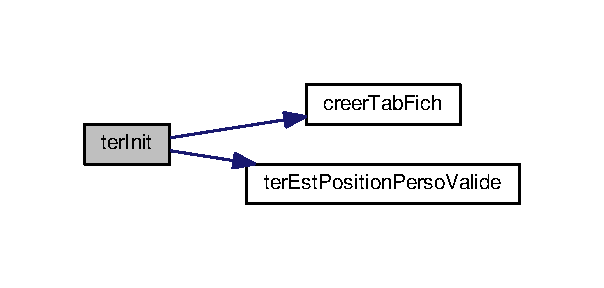
\includegraphics[width=290pt]{_terrain_8c_a44312d3c7ca6ef4573d206043149fc1f_cgraph}
\end{center}
\end{figure}


\hypertarget{_terrain_8c_ac4ec9eb0a375fb3b0d9da191f4af5809}{\index{Terrain.\-c@{Terrain.\-c}!ter\-Libere@{ter\-Libere}}
\index{ter\-Libere@{ter\-Libere}!Terrain.c@{Terrain.\-c}}
\subsubsection[{ter\-Libere}]{\setlength{\rightskip}{0pt plus 5cm}void ter\-Libere (
\begin{DoxyParamCaption}
\item[{{\bf Terrain} $\ast$}]{}
\end{DoxyParamCaption}
)}}\label{_terrain_8c_ac4ec9eb0a375fb3b0d9da191f4af5809}


libere le terrain 


\begin{DoxyParams}{Parameters}
{\em \hyperlink{struct_terrain}{Terrain}} & $\ast$ \\
\hline
\end{DoxyParams}


Definition at line 422 of file Terrain.\-c.



Here is the call graph for this function\-:\nopagebreak
\begin{figure}[H]
\begin{center}
\leavevmode
\includegraphics[width=208pt]{_terrain_8c_ac4ec9eb0a375fb3b0d9da191f4af5809_cgraph}
\end{center}
\end{figure}


\hypertarget{_terrain_8c_a0a32fa4c6166a41d024da8e499fab0cb}{\index{Terrain.\-c@{Terrain.\-c}!ter\-Set\-X\-Y@{ter\-Set\-X\-Y}}
\index{ter\-Set\-X\-Y@{ter\-Set\-X\-Y}!Terrain.c@{Terrain.\-c}}
\subsubsection[{ter\-Set\-X\-Y}]{\setlength{\rightskip}{0pt plus 5cm}void ter\-Set\-X\-Y (
\begin{DoxyParamCaption}
\item[{const {\bf Terrain} $\ast$}]{, }
\item[{const int}]{, }
\item[{const int}]{, }
\item[{const char}]{}
\end{DoxyParamCaption}
)}}\label{_terrain_8c_a0a32fa4c6166a41d024da8e499fab0cb}


change le contenu de la case xy 


\begin{DoxyParams}{Parameters}
{\em \hyperlink{struct_terrain}{Terrain}} & $\ast$ \\
\hline
{\em int} & \\
\hline
{\em char} & \\
\hline
\end{DoxyParams}


Definition at line 536 of file Terrain.\-c.

\hypertarget{_terrain_8c_a65f656bd303453c5fadac03ae22ec70b}{\index{Terrain.\-c@{Terrain.\-c}!vider@{vider}}
\index{vider@{vider}!Terrain.c@{Terrain.\-c}}
\subsubsection[{vider}]{\setlength{\rightskip}{0pt plus 5cm}void vider (
\begin{DoxyParamCaption}
\item[{{\bf Salle} $\ast$}]{n}
\end{DoxyParamCaption}
)}}\label{_terrain_8c_a65f656bd303453c5fadac03ae22ec70b}


Definition at line 427 of file Terrain.\-c.


\hypertarget{_terrain_8h}{\section{/home/enzo/projet\-\_\-fluide/src/\-Terrain.h File Reference}
\label{_terrain_8h}\index{/home/enzo/projet\-\_\-fluide/src/\-Terrain.\-h@{/home/enzo/projet\-\_\-fluide/src/\-Terrain.\-h}}
}
{\ttfamily \#include $<$stdio.\-h$>$}\\*
{\ttfamily \#include $<$stdlib.\-h$>$}\\*
{\ttfamily \#include $<$S\-D\-L/\-S\-D\-L\-\_\-image.\-h$>$}\\*
{\ttfamily \#include $<$S\-D\-L/\-S\-D\-L.\-h$>$}\\*
Include dependency graph for Terrain.\-h\-:\nopagebreak
\begin{figure}[H]
\begin{center}
\leavevmode
\includegraphics[width=350pt]{_terrain_8h__incl}
\end{center}
\end{figure}
This graph shows which files directly or indirectly include this file\-:
\nopagebreak
\begin{figure}[H]
\begin{center}
\leavevmode
\includegraphics[width=350pt]{_terrain_8h__dep__incl}
\end{center}
\end{figure}
\subsection*{Data Structures}
\begin{DoxyCompactItemize}
\item 
struct \hyperlink{struct_fantome}{Fantome}
\begin{DoxyCompactList}\small\item\em Module image. \end{DoxyCompactList}\item 
struct \hyperlink{struct___salle}{\-\_\-\-Salle}
\item 
struct \hyperlink{struct_terrain}{Terrain}
\end{DoxyCompactItemize}
\subsection*{Typedefs}
\begin{DoxyCompactItemize}
\item 
typedef struct \hyperlink{struct___salle}{\-\_\-\-Salle} \hyperlink{_terrain_8h_a00ea6820934a8f863026cfbfad337db8}{Salle}
\end{DoxyCompactItemize}
\subsection*{Functions}
\begin{DoxyCompactItemize}
\item 
void \hyperlink{_terrain_8h_a6d08249ac03deb3b724cfe24bfcd199d}{ter\-Init} (\hyperlink{struct_terrain}{Terrain} $\ast$)
\begin{DoxyCompactList}\small\item\em ter\-Init initialise le terrain \end{DoxyCompactList}\item 
void \hyperlink{_terrain_8h_a6b1c85f63f3b514768066b3b444d81c7}{init\-Fant} (\hyperlink{struct_terrain}{Terrain} $\ast$)
\begin{DoxyCompactList}\small\item\em init\-Fant initialise les ennemis \end{DoxyCompactList}\item 
void \hyperlink{_terrain_8h_a33d953593dec7f7101c0e92aeca4f00e}{ter\-Libere} (\hyperlink{struct_terrain}{Terrain} $\ast$)
\begin{DoxyCompactList}\small\item\em libere le terrain \end{DoxyCompactList}\item 
int \hyperlink{_terrain_8h_a6ee954227217040c6cc35090d4e97748}{ter\-Est\-Position\-Perso\-Valide} (const \hyperlink{struct_terrain}{Terrain} $\ast$, const int, const int)
\begin{DoxyCompactList}\small\item\em ter\-Est\-Pos\-Perso\-Valide regarde si la position d'une entite est conforme au décors \end{DoxyCompactList}\item 
void \hyperlink{_terrain_8h_a145b4f97bb6bda560fca5c014a35934d}{ter\-Actuel\-Initdroite} (\hyperlink{struct_terrain}{Terrain} $\ast$)
\begin{DoxyCompactList}\small\item\em ter\-Actuel\-Initdroite actualise le terrain si le personage est passe pas la porte de droite \end{DoxyCompactList}\item 
void \hyperlink{_terrain_8h_abfe20b802508190569c1afa5bbc30d96}{ter\-Actuel\-Initgauche} (\hyperlink{struct_terrain}{Terrain} $\ast$)
\begin{DoxyCompactList}\small\item\em ter\-Actuel\-Initdroite actualise le terrain si le personage est passe pas la porte de gauche \end{DoxyCompactList}\item 
void \hyperlink{_terrain_8h_a835e5cd3a1db0bfae2dc653fb8d76fc1}{ter\-Actuel\-Inithaut} (\hyperlink{struct_terrain}{Terrain} $\ast$)
\begin{DoxyCompactList}\small\item\em ter\-Actuel\-Initdroite actualise le terrain si le personage est passe pas la porte de haut \end{DoxyCompactList}\item 
void \hyperlink{_terrain_8h_a0803f6751f40cade7a296f1c54d0946e}{ter\-Actuel\-Initbas} (\hyperlink{struct_terrain}{Terrain} $\ast$)
\begin{DoxyCompactList}\small\item\em ter\-Actuel\-Initdroite actualise le terrain si le personage est passe pas la porte de bas \end{DoxyCompactList}\item 
int \hyperlink{_terrain_8h_a7ff92302aa6d2fcd0b10639d450b23aa}{Marqueur\-Present} (const \hyperlink{struct_terrain}{Terrain} $\ast$, const int, const int)
\begin{DoxyCompactList}\small\item\em Marqueur\-Present regarde si il y a un marqueur dans une case precise du tableau si oui, les enemis ne pas peuvent passer. \end{DoxyCompactList}\item 
const char \hyperlink{_terrain_8h_acdf315b17166803bb98fcad61d864267}{ter\-Get\-X\-Y} (const \hyperlink{struct_terrain}{Terrain} $\ast$, const int, const int)
\begin{DoxyCompactList}\small\item\em donne le contenu de la case xy \end{DoxyCompactList}\item 
void \hyperlink{_terrain_8h_a0fc64883b093bd186d9b3619e483a454}{ter\-Set\-X\-Y} (const \hyperlink{struct_terrain}{Terrain} $\ast$, const int, const int, const char)
\begin{DoxyCompactList}\small\item\em change le contenu de la case xy \end{DoxyCompactList}\item 
const int \hyperlink{_terrain_8h_ab2a4c597cc893ff2c7c1b6193f722398}{get\-Dim\-X} (const \hyperlink{struct_terrain}{Terrain} $\ast$)
\begin{DoxyCompactList}\small\item\em donne la taille du terrain \end{DoxyCompactList}\item 
const int \hyperlink{_terrain_8h_a78e20dd48fe85faf3d2c5d20981b17d1}{get\-Dim\-Y} (const \hyperlink{struct_terrain}{Terrain} $\ast$)
\begin{DoxyCompactList}\small\item\em donne la taille du terrain \end{DoxyCompactList}\item 
void \hyperlink{_terrain_8h_a7ca257e9f8be253422eeff398ed1153a}{perso\-Proche\-Rat} (const \hyperlink{struct_terrain}{Terrain} $\ast$, const int, const int)
\begin{DoxyCompactList}\small\item\em regarde si le personnage est proche des ennemis \end{DoxyCompactList}\item 
void \hyperlink{_terrain_8h_acb53f00b7ac91cca4fcd22d5be6d58b8}{mode\-Agro} (const \hyperlink{struct_terrain}{Terrain} $\ast$, const int, const int, const int)
\begin{DoxyCompactList}\small\item\em fait en sorte que les ennemis attaquent le personnage \end{DoxyCompactList}\item 
const int \hyperlink{_terrain_8h_af5d683f812d1747c4833083ead28c7e5}{getnbfant} (const \hyperlink{struct_terrain}{Terrain} $\ast$)
\begin{DoxyCompactList}\small\item\em regarde le nombre d'ennemis dans une salle \end{DoxyCompactList}\item 
int \hyperlink{_terrain_8h_a9501a8043ac3eb836e4a5da1b8119c07}{ter\-Est\-Position\-Perso\-Pic} (const \hyperlink{struct_terrain}{Terrain} $\ast$, const int, const int)
\begin{DoxyCompactList}\small\item\em regarde si le personnage marche sur un pique \end{DoxyCompactList}\end{DoxyCompactItemize}


\subsection{Typedef Documentation}
\hypertarget{_terrain_8h_a00ea6820934a8f863026cfbfad337db8}{\index{Terrain.\-h@{Terrain.\-h}!Salle@{Salle}}
\index{Salle@{Salle}!Terrain.h@{Terrain.\-h}}
\subsubsection[{Salle}]{\setlength{\rightskip}{0pt plus 5cm}typedef struct {\bf \-\_\-\-Salle}  {\bf Salle}}}\label{_terrain_8h_a00ea6820934a8f863026cfbfad337db8}


\subsection{Function Documentation}
\hypertarget{_terrain_8h_ab2a4c597cc893ff2c7c1b6193f722398}{\index{Terrain.\-h@{Terrain.\-h}!get\-Dim\-X@{get\-Dim\-X}}
\index{get\-Dim\-X@{get\-Dim\-X}!Terrain.h@{Terrain.\-h}}
\subsubsection[{get\-Dim\-X}]{\setlength{\rightskip}{0pt plus 5cm}const int get\-Dim\-X (
\begin{DoxyParamCaption}
\item[{const {\bf Terrain} $\ast$}]{}
\end{DoxyParamCaption}
)}}\label{_terrain_8h_ab2a4c597cc893ff2c7c1b6193f722398}


donne la taille du terrain 


\begin{DoxyParams}{Parameters}
{\em \hyperlink{struct_terrain}{Terrain}} & $\ast$ \\
\hline
\end{DoxyParams}


Definition at line 545 of file Terrain.\-c.

\hypertarget{_terrain_8h_a78e20dd48fe85faf3d2c5d20981b17d1}{\index{Terrain.\-h@{Terrain.\-h}!get\-Dim\-Y@{get\-Dim\-Y}}
\index{get\-Dim\-Y@{get\-Dim\-Y}!Terrain.h@{Terrain.\-h}}
\subsubsection[{get\-Dim\-Y}]{\setlength{\rightskip}{0pt plus 5cm}const int get\-Dim\-Y (
\begin{DoxyParamCaption}
\item[{const {\bf Terrain} $\ast$}]{}
\end{DoxyParamCaption}
)}}\label{_terrain_8h_a78e20dd48fe85faf3d2c5d20981b17d1}


donne la taille du terrain 


\begin{DoxyParams}{Parameters}
{\em \hyperlink{struct_terrain}{Terrain}} & $\ast$ \\
\hline
\end{DoxyParams}


Definition at line 550 of file Terrain.\-c.

\hypertarget{_terrain_8h_af5d683f812d1747c4833083ead28c7e5}{\index{Terrain.\-h@{Terrain.\-h}!getnbfant@{getnbfant}}
\index{getnbfant@{getnbfant}!Terrain.h@{Terrain.\-h}}
\subsubsection[{getnbfant}]{\setlength{\rightskip}{0pt plus 5cm}const int getnbfant (
\begin{DoxyParamCaption}
\item[{const {\bf Terrain} $\ast$}]{}
\end{DoxyParamCaption}
)}}\label{_terrain_8h_af5d683f812d1747c4833083ead28c7e5}


regarde le nombre d'ennemis dans une salle 


\begin{DoxyParams}{Parameters}
{\em \hyperlink{struct_terrain}{Terrain}} & $\ast$ \\
\hline
\end{DoxyParams}


Definition at line 555 of file Terrain.\-c.

\hypertarget{_terrain_8h_a6b1c85f63f3b514768066b3b444d81c7}{\index{Terrain.\-h@{Terrain.\-h}!init\-Fant@{init\-Fant}}
\index{init\-Fant@{init\-Fant}!Terrain.h@{Terrain.\-h}}
\subsubsection[{init\-Fant}]{\setlength{\rightskip}{0pt plus 5cm}void init\-Fant (
\begin{DoxyParamCaption}
\item[{{\bf Terrain} $\ast$}]{}
\end{DoxyParamCaption}
)}}\label{_terrain_8h_a6b1c85f63f3b514768066b3b444d81c7}


init\-Fant initialise les ennemis 


\begin{DoxyParams}{Parameters}
{\em \hyperlink{struct_terrain}{Terrain}} & $\ast$ \\
\hline
\end{DoxyParams}


Definition at line 310 of file Terrain.\-c.



Here is the call graph for this function\-:\nopagebreak
\begin{figure}[H]
\begin{center}
\leavevmode
\includegraphics[width=298pt]{_terrain_8h_a6b1c85f63f3b514768066b3b444d81c7_cgraph}
\end{center}
\end{figure}


\hypertarget{_terrain_8h_a7ff92302aa6d2fcd0b10639d450b23aa}{\index{Terrain.\-h@{Terrain.\-h}!Marqueur\-Present@{Marqueur\-Present}}
\index{Marqueur\-Present@{Marqueur\-Present}!Terrain.h@{Terrain.\-h}}
\subsubsection[{Marqueur\-Present}]{\setlength{\rightskip}{0pt plus 5cm}int Marqueur\-Present (
\begin{DoxyParamCaption}
\item[{const {\bf Terrain} $\ast$}]{, }
\item[{const int}]{, }
\item[{const int}]{}
\end{DoxyParamCaption}
)}}\label{_terrain_8h_a7ff92302aa6d2fcd0b10639d450b23aa}


Marqueur\-Present regarde si il y a un marqueur dans une case precise du tableau si oui, les enemis ne pas peuvent passer. 


\begin{DoxyParams}{Parameters}
{\em \hyperlink{struct_terrain}{Terrain}} & $\ast$ \\
\hline
{\em int} & \\
\hline
{\em int} & \\
\hline
\end{DoxyParams}


Definition at line 511 of file Terrain.\-c.

\hypertarget{_terrain_8h_acb53f00b7ac91cca4fcd22d5be6d58b8}{\index{Terrain.\-h@{Terrain.\-h}!mode\-Agro@{mode\-Agro}}
\index{mode\-Agro@{mode\-Agro}!Terrain.h@{Terrain.\-h}}
\subsubsection[{mode\-Agro}]{\setlength{\rightskip}{0pt plus 5cm}void mode\-Agro (
\begin{DoxyParamCaption}
\item[{const {\bf Terrain} $\ast$}]{, }
\item[{const int}]{, }
\item[{const int}]{, }
\item[{const int}]{}
\end{DoxyParamCaption}
)}}\label{_terrain_8h_acb53f00b7ac91cca4fcd22d5be6d58b8}


fait en sorte que les ennemis attaquent le personnage 


\begin{DoxyParams}{Parameters}
{\em \hyperlink{struct_terrain}{Terrain}} & $\ast$ \\
\hline
{\em int} & \\
\hline
{\em int} & \\
\hline
{\em int} & \\
\hline
\end{DoxyParams}


Definition at line 486 of file Terrain.\-c.



Here is the call graph for this function\-:\nopagebreak
\begin{figure}[H]
\begin{center}
\leavevmode
\includegraphics[width=226pt]{_terrain_8h_acb53f00b7ac91cca4fcd22d5be6d58b8_cgraph}
\end{center}
\end{figure}


\hypertarget{_terrain_8h_a7ca257e9f8be253422eeff398ed1153a}{\index{Terrain.\-h@{Terrain.\-h}!perso\-Proche\-Rat@{perso\-Proche\-Rat}}
\index{perso\-Proche\-Rat@{perso\-Proche\-Rat}!Terrain.h@{Terrain.\-h}}
\subsubsection[{perso\-Proche\-Rat}]{\setlength{\rightskip}{0pt plus 5cm}void perso\-Proche\-Rat (
\begin{DoxyParamCaption}
\item[{const {\bf Terrain} $\ast$}]{, }
\item[{const int}]{, }
\item[{const int}]{}
\end{DoxyParamCaption}
)}}\label{_terrain_8h_a7ca257e9f8be253422eeff398ed1153a}


regarde si le personnage est proche des ennemis 


\begin{DoxyParams}{Parameters}
{\em \hyperlink{struct_terrain}{Terrain}} & $\ast$ \\
\hline
{\em int} & \\
\hline
{\em int} & \\
\hline
\end{DoxyParams}


Definition at line 464 of file Terrain.\-c.

\hypertarget{_terrain_8h_a0803f6751f40cade7a296f1c54d0946e}{\index{Terrain.\-h@{Terrain.\-h}!ter\-Actuel\-Initbas@{ter\-Actuel\-Initbas}}
\index{ter\-Actuel\-Initbas@{ter\-Actuel\-Initbas}!Terrain.h@{Terrain.\-h}}
\subsubsection[{ter\-Actuel\-Initbas}]{\setlength{\rightskip}{0pt plus 5cm}void ter\-Actuel\-Initbas (
\begin{DoxyParamCaption}
\item[{{\bf Terrain} $\ast$}]{}
\end{DoxyParamCaption}
)}}\label{_terrain_8h_a0803f6751f40cade7a296f1c54d0946e}


ter\-Actuel\-Initdroite actualise le terrain si le personage est passe pas la porte de bas 


\begin{DoxyParams}{Parameters}
{\em \hyperlink{struct_terrain}{Terrain}} & $\ast$ \\
\hline
\end{DoxyParams}


Definition at line 393 of file Terrain.\-c.

\hypertarget{_terrain_8h_a145b4f97bb6bda560fca5c014a35934d}{\index{Terrain.\-h@{Terrain.\-h}!ter\-Actuel\-Initdroite@{ter\-Actuel\-Initdroite}}
\index{ter\-Actuel\-Initdroite@{ter\-Actuel\-Initdroite}!Terrain.h@{Terrain.\-h}}
\subsubsection[{ter\-Actuel\-Initdroite}]{\setlength{\rightskip}{0pt plus 5cm}void ter\-Actuel\-Initdroite (
\begin{DoxyParamCaption}
\item[{{\bf Terrain} $\ast$}]{}
\end{DoxyParamCaption}
)}}\label{_terrain_8h_a145b4f97bb6bda560fca5c014a35934d}


ter\-Actuel\-Initdroite actualise le terrain si le personage est passe pas la porte de droite 


\begin{DoxyParams}{Parameters}
{\em \hyperlink{struct_terrain}{Terrain}} & $\ast$ \\
\hline
\end{DoxyParams}


Definition at line 336 of file Terrain.\-c.

\hypertarget{_terrain_8h_abfe20b802508190569c1afa5bbc30d96}{\index{Terrain.\-h@{Terrain.\-h}!ter\-Actuel\-Initgauche@{ter\-Actuel\-Initgauche}}
\index{ter\-Actuel\-Initgauche@{ter\-Actuel\-Initgauche}!Terrain.h@{Terrain.\-h}}
\subsubsection[{ter\-Actuel\-Initgauche}]{\setlength{\rightskip}{0pt plus 5cm}void ter\-Actuel\-Initgauche (
\begin{DoxyParamCaption}
\item[{{\bf Terrain} $\ast$}]{}
\end{DoxyParamCaption}
)}}\label{_terrain_8h_abfe20b802508190569c1afa5bbc30d96}


ter\-Actuel\-Initdroite actualise le terrain si le personage est passe pas la porte de gauche 


\begin{DoxyParams}{Parameters}
{\em \hyperlink{struct_terrain}{Terrain}} & $\ast$ \\
\hline
\end{DoxyParams}


Definition at line 356 of file Terrain.\-c.

\hypertarget{_terrain_8h_a835e5cd3a1db0bfae2dc653fb8d76fc1}{\index{Terrain.\-h@{Terrain.\-h}!ter\-Actuel\-Inithaut@{ter\-Actuel\-Inithaut}}
\index{ter\-Actuel\-Inithaut@{ter\-Actuel\-Inithaut}!Terrain.h@{Terrain.\-h}}
\subsubsection[{ter\-Actuel\-Inithaut}]{\setlength{\rightskip}{0pt plus 5cm}void ter\-Actuel\-Inithaut (
\begin{DoxyParamCaption}
\item[{{\bf Terrain} $\ast$}]{}
\end{DoxyParamCaption}
)}}\label{_terrain_8h_a835e5cd3a1db0bfae2dc653fb8d76fc1}


ter\-Actuel\-Initdroite actualise le terrain si le personage est passe pas la porte de haut 


\begin{DoxyParams}{Parameters}
{\em \hyperlink{struct_terrain}{Terrain}} & $\ast$ \\
\hline
\end{DoxyParams}


Definition at line 374 of file Terrain.\-c.

\hypertarget{_terrain_8h_a9501a8043ac3eb836e4a5da1b8119c07}{\index{Terrain.\-h@{Terrain.\-h}!ter\-Est\-Position\-Perso\-Pic@{ter\-Est\-Position\-Perso\-Pic}}
\index{ter\-Est\-Position\-Perso\-Pic@{ter\-Est\-Position\-Perso\-Pic}!Terrain.h@{Terrain.\-h}}
\subsubsection[{ter\-Est\-Position\-Perso\-Pic}]{\setlength{\rightskip}{0pt plus 5cm}int ter\-Est\-Position\-Perso\-Pic (
\begin{DoxyParamCaption}
\item[{const {\bf Terrain} $\ast$}]{, }
\item[{const int}]{, }
\item[{const int}]{}
\end{DoxyParamCaption}
)}}\label{_terrain_8h_a9501a8043ac3eb836e4a5da1b8119c07}


regarde si le personnage marche sur un pique 


\begin{DoxyParams}{Parameters}
{\em Terrain$\ast$} & \\
\hline
{\em const} & int \\
\hline
{\em const} & int \\
\hline
\end{DoxyParams}


Definition at line 448 of file Terrain.\-c.

\hypertarget{_terrain_8h_a6ee954227217040c6cc35090d4e97748}{\index{Terrain.\-h@{Terrain.\-h}!ter\-Est\-Position\-Perso\-Valide@{ter\-Est\-Position\-Perso\-Valide}}
\index{ter\-Est\-Position\-Perso\-Valide@{ter\-Est\-Position\-Perso\-Valide}!Terrain.h@{Terrain.\-h}}
\subsubsection[{ter\-Est\-Position\-Perso\-Valide}]{\setlength{\rightskip}{0pt plus 5cm}int ter\-Est\-Position\-Perso\-Valide (
\begin{DoxyParamCaption}
\item[{const {\bf Terrain} $\ast$}]{, }
\item[{const int}]{, }
\item[{const int}]{}
\end{DoxyParamCaption}
)}}\label{_terrain_8h_a6ee954227217040c6cc35090d4e97748}


ter\-Est\-Pos\-Perso\-Valide regarde si la position d'une entite est conforme au décors 


\begin{DoxyParams}{Parameters}
{\em \hyperlink{struct_terrain}{Terrain}} & $\ast$ \\
\hline
{\em int} & \\
\hline
{\em int} & \\
\hline
\end{DoxyParams}


Definition at line 440 of file Terrain.\-c.

\hypertarget{_terrain_8h_acdf315b17166803bb98fcad61d864267}{\index{Terrain.\-h@{Terrain.\-h}!ter\-Get\-X\-Y@{ter\-Get\-X\-Y}}
\index{ter\-Get\-X\-Y@{ter\-Get\-X\-Y}!Terrain.h@{Terrain.\-h}}
\subsubsection[{ter\-Get\-X\-Y}]{\setlength{\rightskip}{0pt plus 5cm}const char ter\-Get\-X\-Y (
\begin{DoxyParamCaption}
\item[{const {\bf Terrain} $\ast$}]{, }
\item[{const int}]{, }
\item[{const int}]{}
\end{DoxyParamCaption}
)}}\label{_terrain_8h_acdf315b17166803bb98fcad61d864267}


donne le contenu de la case xy 


\begin{DoxyParams}{Parameters}
{\em \hyperlink{struct_terrain}{Terrain}} & $\ast$ \\
\hline
{\em int} & \\
\hline
{\em int} & \\
\hline
\end{DoxyParams}


Definition at line 527 of file Terrain.\-c.

\hypertarget{_terrain_8h_a6d08249ac03deb3b724cfe24bfcd199d}{\index{Terrain.\-h@{Terrain.\-h}!ter\-Init@{ter\-Init}}
\index{ter\-Init@{ter\-Init}!Terrain.h@{Terrain.\-h}}
\subsubsection[{ter\-Init}]{\setlength{\rightskip}{0pt plus 5cm}void ter\-Init (
\begin{DoxyParamCaption}
\item[{{\bf Terrain} $\ast$}]{}
\end{DoxyParamCaption}
)}}\label{_terrain_8h_a6d08249ac03deb3b724cfe24bfcd199d}


ter\-Init initialise le terrain 


\begin{DoxyParams}{Parameters}
{\em \hyperlink{struct_terrain}{Terrain}} & $\ast$ \\
\hline
\end{DoxyParams}


Definition at line 6 of file Terrain.\-c.



Here is the call graph for this function\-:\nopagebreak
\begin{figure}[H]
\begin{center}
\leavevmode
\includegraphics[width=290pt]{_terrain_8h_a6d08249ac03deb3b724cfe24bfcd199d_cgraph}
\end{center}
\end{figure}


\hypertarget{_terrain_8h_a33d953593dec7f7101c0e92aeca4f00e}{\index{Terrain.\-h@{Terrain.\-h}!ter\-Libere@{ter\-Libere}}
\index{ter\-Libere@{ter\-Libere}!Terrain.h@{Terrain.\-h}}
\subsubsection[{ter\-Libere}]{\setlength{\rightskip}{0pt plus 5cm}void ter\-Libere (
\begin{DoxyParamCaption}
\item[{{\bf Terrain} $\ast$}]{}
\end{DoxyParamCaption}
)}}\label{_terrain_8h_a33d953593dec7f7101c0e92aeca4f00e}


libere le terrain 


\begin{DoxyParams}{Parameters}
{\em \hyperlink{struct_terrain}{Terrain}} & $\ast$ \\
\hline
\end{DoxyParams}


Definition at line 422 of file Terrain.\-c.



Here is the call graph for this function\-:\nopagebreak
\begin{figure}[H]
\begin{center}
\leavevmode
\includegraphics[width=208pt]{_terrain_8h_a33d953593dec7f7101c0e92aeca4f00e_cgraph}
\end{center}
\end{figure}


\hypertarget{_terrain_8h_a0fc64883b093bd186d9b3619e483a454}{\index{Terrain.\-h@{Terrain.\-h}!ter\-Set\-X\-Y@{ter\-Set\-X\-Y}}
\index{ter\-Set\-X\-Y@{ter\-Set\-X\-Y}!Terrain.h@{Terrain.\-h}}
\subsubsection[{ter\-Set\-X\-Y}]{\setlength{\rightskip}{0pt plus 5cm}void ter\-Set\-X\-Y (
\begin{DoxyParamCaption}
\item[{const {\bf Terrain} $\ast$}]{, }
\item[{const int}]{, }
\item[{const int}]{, }
\item[{const char}]{}
\end{DoxyParamCaption}
)}}\label{_terrain_8h_a0fc64883b093bd186d9b3619e483a454}


change le contenu de la case xy 


\begin{DoxyParams}{Parameters}
{\em \hyperlink{struct_terrain}{Terrain}} & $\ast$ \\
\hline
{\em int} & \\
\hline
{\em char} & \\
\hline
\end{DoxyParams}


Definition at line 536 of file Terrain.\-c.


%--- End generated contents ---

% Index
\newpage
\phantomsection
\addcontentsline{toc}{chapter}{Index}
\printindex

\end{document}
